\chapter{RESULTS AND DISCUSSIONS}


\section{CHAPTER ORGANIZATION}


\subsection{Result comparisons with Published Reference Paper}

This section discusses the results of this work in comparison to the published reference paper by \cite{Zhong-etal:2018}, titled "A realtime interpolator for parametric curves". The results in this work showed similar patterns and comparable values to the published referenced results. The comparisons cover the feedrate variations along the curve, the velocity profiles of the x and y axes motions, the current running feedrate profile against the feedrate-limit,  and the acceleration profile.  These results spanned the entire traversal along the parametric curve. 
  

\subsection{Algorithm Executions}

This section discusses the total number of algorithm executions, history of algorithm revisions, selection of an illustrative curve among the ten(10) parametric curves, acceleration jitters, and determination of the acceptable or nominal value of the acceleration safety factor lamda to avoid acceleration jitters.  

\subsection{Teardrop Curve for Illustration}

This section describes the characteristics of the Teardrop curve, and the basic reasons for making the Teardrop curve as an illustration curve. The rest of the nine(9) curves are described in comparison to the Teardrop curve.

\subsection{Results of Teardrop curve}

This section discusses the full outputs of the Teardrop curve resulting from the algorithm execution. Similar outputs for the rest of the nine(9) curves are provided in their respective appendices.\\

These illustrative outputs cover, for example, the direction of travel for the curve, the radius of curvature rho(u), the first and second-order terms in Taylor's expansion, the chord-error absolute constraint, the running feedrate absolute constraint, the four(4) components of the feedrate limit, histogram distribution of interpolated points, starting and ending feedrate profiles, color coded running feedrates and many more.

\subsection{Notable Results for Rest of Curves}

This section discusses specific aspects of the execution results worthy of further clarification. Four(4) special cases were considered. Results of the Circle and Ellipse curves that can be used as a means of validation and verification of algorithm performance were highlighted. Results that look abnormal but are correct need to be explained. This cover negative results for the difference (SAL-SCL) in the Teardrop curve, and machine epsilon problems for the SnaHyp curve. 

\subsection{Overall Execution Results}

This section presents the algorithm execution summary results for all of the ten(10) parametric curves studied in this work. The discussions include the Feedrate Command (FC) and the Lamda safety factor (LSF), algorithm validation and verification (V \& V), LinuxCNC-Axis simulation run validation (SRV), real run validation on the CNC machine (RRV), and algorithm performance measures.\\

The performance measures cover algorithm generated variables like total interpolated points (TIP), total sum-arc-length (SAL), total sum-chord-length (SCL), total sum-chord-error (SCE), total sum-arc-theta (SAT), and total sum-arc-area (SAA). \\

The four(4) assessment metrics for algorithm performance are: (SCE/TIP), (SCE/SCL), (SAA/SCL) and 100*(SAL-SCL)/SAL. The first three terms are ratios while last term is a percentage measure of the difference.


\subsection{Summary of Results Chapter}
 
This section summarizes the important findings in this chapter.\\

\noindent
\textbf{IMPORTANT NOTE}: Some data tables and graphs are displayed in landscape mode, when it is not possible in portrait mode. The landscape mode facilitates presentation of multiple plots side by side, including and especially wide data tables. This mode helps comprehension, visualization and comparison of information.

% ========================================================
\clearpage
\pagebreak
%% \begin{landscape} 

\section{COMPARISONS AGAINST PUBLISHED PAPER}

\subsection{Result comparisons with Published Reference Paper}

It is important to note that the comparisons of results in this work can only be made against the Teardrop parametric curve in the referenced paper by \cite{Zhong-etal:2018}, because this work uses the same parametric equation. And it must also be reminded that the single interpolation algorithm designed and developed in this work is to cater ten(10) different parametric curves of various features, shapes and dimensions, not just the one simple Teardrop curve. \\

The computational algorithms are also different between this work and the published paper. The overall algorithm in this work is considered simpler (not complicated branching flow), highly structured (for example, one-way-in and one-way-out for every computing unit), and therefore easy to understand and maintain. In addition, this algorithm strictly enforces complete and simultaneous non-violation of chord-error and feedrate-limit constraints. The results is absolute success when applied to all ten(10) different parametric curves. \\   

For the above reasons, it cannot be said that the algorithm is an-apple-to-apple comparison with that of the published paper, even for the identical Teardrop curve. Obviously, the computation techniques are different. However, the common theme is that both are "interpolation algorithms", meaning given a current point on the parametric curve, find the next point for the move on the curve. These are the reasons it was stated that the results in this work showed similar patterns and comparable values. The comparisons are described in the next section.

%% ===========================================================
\clearpage
\pagebreak
%% \begin{landscape} 

\subsection{Display comparison results}

\noindent The four(4) comparisons for the Teardrop curve cover : \\
\noindent 
(1) Feedrate variations along the curve shown in Fig[\ref{img-Feedrate variations along the curve}].\\
(2) Velocity profiles of the x and y axes motions shown in Fig[\ref{img-Comparisons velocity profiles of the x and y axes motions}].\\
(3) Running feedrate profile against the feedrate-limit shown in Fig[\ref{img-Running feedrate profile against the feedrate-limit}].\\  
(4) Acceleration profile containment shown in Fig[\ref{img-Acceleration profile containment}].


\subsection{Discussion on comparative results}

\noindent It is important to note that This-Work (PhD thesis) provides results that are similar and comparable to the work produced in the Reference-Paper. This comparison is only applicable to the Teardrop because both adopted the same exact equation for the parametric curve. The four(4) figures for comparison in the next section are provided in landscape mode. The legend colors of the curves displayed in the figures were made identical for easy visual comparison. \\

\noindent
In Fig[\ref{img-Feedrate variations along the curve}], the feedrate variations in the interpolation are similar and comparable. The generally lower feedrate values in This-Work as the (x, y) position point moves along the Teardrop trajectory is due to both the simultaneous absolute constraints on chord-error (epsilon) and non-violation of the machine feedrate limit. In the Reference-Paper, there is a push-up of the running feedrate, which causes an increase in chord-length, thereby an increase in chord-error. In the Reference-Paper there is no specific mention of absolutely restricting the chord-error for each interpolation point in parameter (u).\\ 

\noindent
Also in Fig[\ref{img-Feedrate variations along the curve}], the different colors refer to the magnitudes of the feedrate (mm/s), which varies from point-to-point on the parametric curve. In this work, the colors transition smoothly following the color spectrum. There is no jumping of colors. The direction of travel of the (x, y) point is starting from the apex going counter-clockwise. \\

\noindent 
In Fig[\ref{img-Comparisons velocity profiles of the x and y axes motions}], the velocity profiles of the x and y axes motions are also similar and comparable. However, the number of interpolated points in This-Work (7599 points) is higher than the Reference-Paper. See the x-axis for the runtime in seconds. Each cycle of interpolated points is set the same for both works, that is, at 0.001 (s) or one millisecond. This makes the completion time for the interpolation algorithm in This-Work as 7.6 seconds, while that for the Reference-Paper as about 6.3 seconds.\\   

\noindent
In Fig[\ref{img-Running feedrate profile against the feedrate-limit}], the actual running feedrate (velocity) almost overlaps with the machine feedrate limit calculated by the algorithm. The feedrate determination is one of the most important and difficult computation to handle. It is a combined effect of both dynamical and kinematical constraints which varies among different CNC machines. \\

\noindent 
Also in Fig[\ref{img-Running feedrate profile against the feedrate-limit}], with the exception of the initial rise and final fall of the actual feedrates, the middle section shows that in both the Reference-Paper and This-Work, the actual running feedrate follows exactly the value of feedrate limit calculated by the algorithm. In this middle region, it is almost overlapping. The actual initial rise and final fall of the actual feedrates are user-selected S-curves. In This-Work, the initial S-curve-rise region is set at (u = 0.00 to 0.05) and the final S-curve-fall region is set at (u = 0.95 to 1.00). In the Reference-Paper, the characteristics of both S-curve-rise and S-curve-fall regions are not specifically mentioned. \\

\noindent
In Fig[\ref{img-Acceleration profile containment}], the actual running tangential acceleration is constrained within the minimum and maximum accelerations in both the Reference-Paper and This-Work results. The acceleration values are not identical but comparable. The feature for acceleration constraints (min, max) is similar. In This-Work, the value of lambda (acceleration safety factor) was selected to be 0.18, chosen to eliminate acceleration jitters that causes machine velocity jerks. This number 0.18 is good when applied to all ten(10) different parametric curves covered in This-Work. In the Reference-Paper, it was only mentioned that lambda should be within (0.00 and 1.00). The determination of acceptable lambda (acceleration safety factor) is discussed in detail in Section [\ref{chap4-Determination of acceptablel lamda}] in this chapter.  

%% \end{landscape}
%% ===========================================================
\clearpage
\pagebreak
\begin{landscape} 
	
\begin{figure}
	\centering
	\caption  {Feedrate variations along the curve}
	\label{img-Feedrate variations along the curve}
	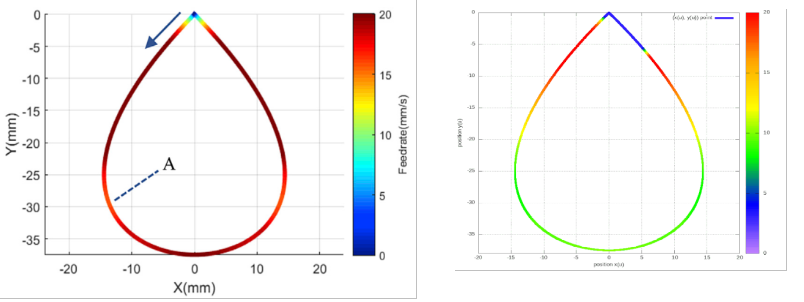
\includegraphics[width= 1.40\textwidth]{Chap4/Comparisons/01-Comparison-Feedrate-Variations-Along-The-Curve.png} 
\end{figure}		

\noindent
\textbf{Equivalent legend}: Reference-Paper (left figure) versus This-Work (right figure)\\

\end{landscape}
% ========================================================
\clearpage
\pagebreak
\begin{landscape} 

\begin{figure}
	\centering
	\caption  {Comparisons velocity profiles of the x and y axes motions}
	\label{img-Comparisons velocity profiles of the x and y axes motions}
	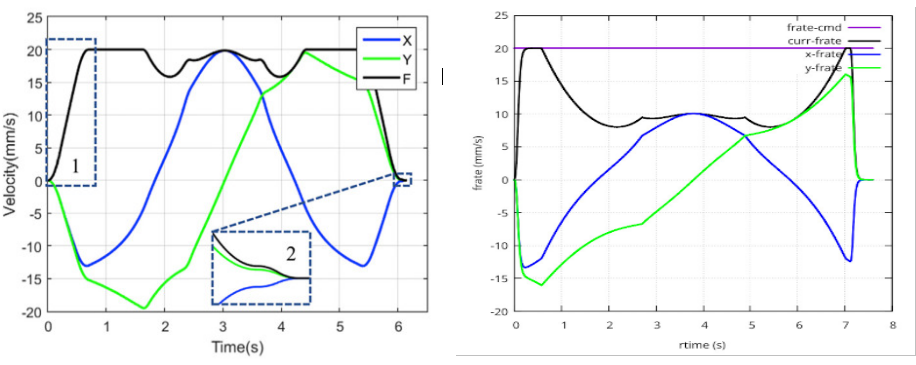
\includegraphics[width= 1.40\textwidth]{Chap4/Comparisons/02-Comparison-Feedrate-Profiles-X-and-Y-Axes.png} 
\end{figure}		

\noindent
\textbf{Equivalent legend}: Reference-Paper (left figure) versus This-Work (right figure)\\
F = curr-frate (Current running feedrate)\\
X = x-frate (X-axis feedrate)\\
Y = y-frate (Y-axis feedrate)\\
Time = rtime (Runtime)\\

\end{landscape}


%% ===========================================================
\clearpage
\pagebreak
\begin{landscape} 
	
\begin{figure}
\centering
\caption  {Running feedrate profile against the feedrate-limit}
\label{img-Running feedrate profile against the feedrate-limit}
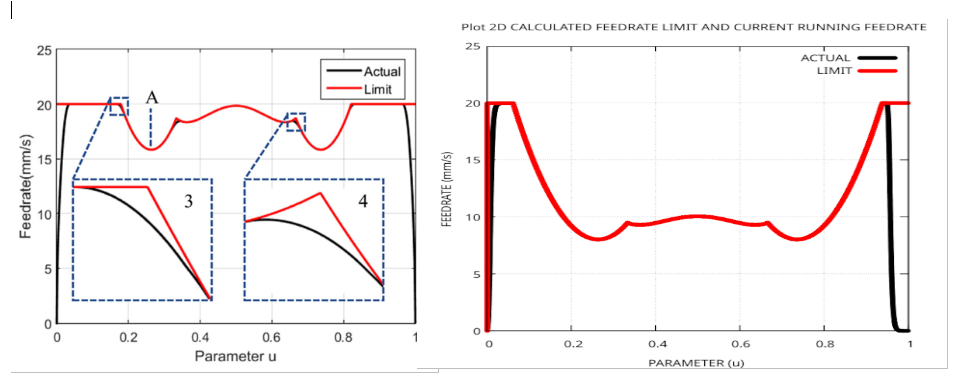
\includegraphics[width= 1.50\textwidth]{Chap4/Comparisons/03-Comparison-Running-feedrate-profile-against-the-feedrate-limit.png} 
\end{figure}		
	
\noindent
\textbf{Equivalent legend}: Reference-Paper (left figure) versus This-Work (right figure)\\


\end{landscape}

%% ===========================================================
\clearpage
\pagebreak
\begin{landscape} 
	
\begin{figure}
\centering
\caption  {Acceleration profile containment}
\label{img-Acceleration profile containment}
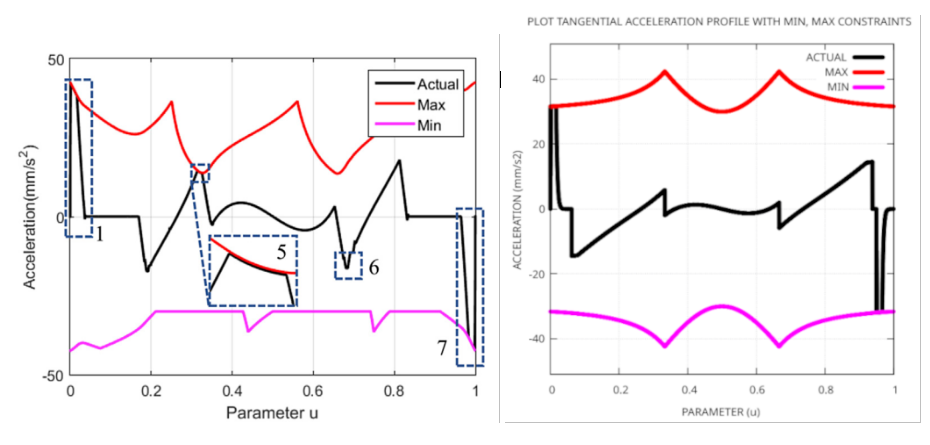
\includegraphics[width= 1.30\textwidth]{Chap4/Comparisons/04-Comparison-Acceleration-profile-containment.png} 
\end{figure}		
	
\noindent
\textbf{Equivalent legend}: Reference-Paper (left figure) versus This-Work (right figure)\\


\end{landscape}
% ========================================================
% ========================================================
\clearpage
\pagebreak

\subsection{Validation of Teardrop curve on CNC machine}

\noindent The following are runtime characteristics of the Teardrop curve computed by the interpolation algorithm for FC20, the Feedrate Command and Lamda = 0.18, the acceleration safety factor. 

\begin{enumerate}
\item Width  (mm)   = 28.8
\item Height (mm)   = 37.5
\item Total interpolated points   = 7599
\item Sum Total arc   length (mm) = 101.8418663504 
\item Sum Total chord-length (mm) = 101.8418655699 
\item Sum Total chord-error  (mm) = 0.007140807163 
\item Average chord-length   (mm) = 0.013403772778 	
\end{enumerate}

\noindent Notice that the CNC machine moves about 7600 incremental steps to cover the distance of 102 mm (about 4 inches) of the total Teardrop curve. This step move is very small indeed, maintaining chord-error below 1 (nm) nanometer and speed (feedrate) below the feedrate limit throughout the entire curve. The average chord-length or linear move per step is 0.0134 (mm). It is quite remarkable that the simple CNC machine is capable of the very small increments. \\

\noindent A snapshot of the CNC machine in operation is shown in Fig[\ref{img-Execution of Teardrop Curve on CNC Machine}] on the next page. A simple pen is used to trace the trajectory of the Teardrop curve. The results for the completed execution of the Teardrop curve is shown next in Fig[\ref{img-Results of Teardrop Curve CNC Machine execution}]. The run was repeated twice for confirmation of correctness.

%% ===========================================================
\clearpage
\pagebreak
%% \begin{landscape} 

%% Left: 01-Teardrop-run-on-CNC-Machine.png
%% Right: 02-Teardrop-run-on-CNC-Machine.png	

\begin{figure}
	\centering
	\caption  {Execution of Teardrop Curve on CNC Machine}
	\label{img-Execution of Teardrop Curve on CNC Machine}
	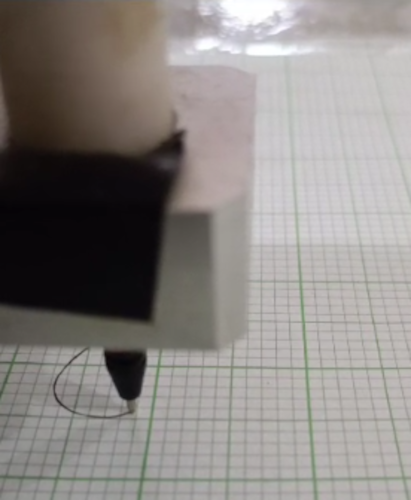
\includegraphics[width=0.60\textwidth]{Chap4/Validation/01-Teardrop-run-on-CNC-Machine.png} 
\end{figure}	

\begin{figure}
	\centering
	\caption  {Results of Teardrop Curve CNC Machine execution - ruler (cm)}
	\label{img-Results of Teardrop Curve CNC Machine execution}
	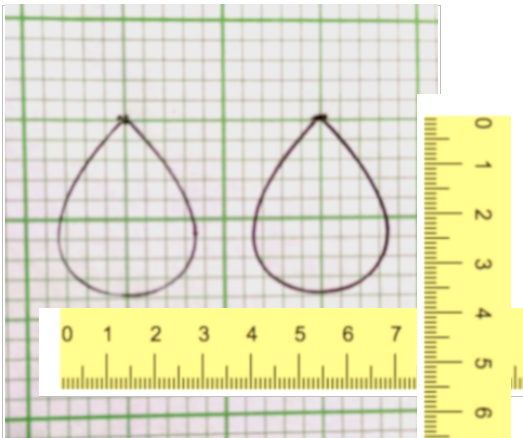
\includegraphics[width=0.70\textwidth]{Chap4/Validation/02-Teardrop-run-on-CNC-Machine.png} 
\end{figure}

	
%% \end{landscape}
% ========================================================
% ========================================================
\clearpage
\pagebreak
%% \begin{landscape} 


\section{ALGORITHM EXECUTIONS}

\subsection{Total algorithm executions}

In this work we have executed the algorithm for ten(10) different curves, four(4) different feedrate commands (FC 10, 20, 30, 40), and four(4) different Lamda safety factors (Lamda 0.10, 0.18, 0.20, 0.50). This combination makes the total number of algorithm executions at 160. For each execution, 3 different input parameters are required, that is, curve type selected, feedrate command FC, and Lamda safety factor. \\

It is expected that a variety of issues arise in these executions due to the diverse characteristics and sizes of the ten(10) curves, the different running feedrates against the machine limits, and the most suitable value of the Lamda safety factor. These interesting issues will be discussed in the forthcoming sections.  

\subsection{Algorithm revisions}

The current revision of the realtime interpolation algorithm is major version 28. The algorithm version 1 started in June, 2022. The software architecture was completed at version 10 by September, 2022 (3 months). Software coding implementation in C/C++ programming language was completed by version 15 in December, 2022 (3 months). Unit and system testing were finished in version 20 by March, 2023 (3 months). Writing major program reports, plotting, recording execution to files, took another 3 months until June, 2023, arriving at version 25. Finally, the full execution of 160 runs, with minor revisions along the way, ended up with the 28th version. This is the state of the software as of October, 2023.     

%% \end{landscape}
%% ===========================================================
\clearpage
\pagebreak

\subsection{Illustrative example Teardrop curve execution} \label{sec-Illustrative example Teardrop curve execution}

\begin{figure}
	\caption  {Teardrop Perspective View 3D in LinuxCNC-Axis}
	\label{img-Chap4-Teardrop-Perspective-View-3D-from-LinuxCNC-Axis.pdf}
	\centering
	\framebox{\includegraphics[width=1.00\textwidth]{Chap4/illustration/img-Teardrop-Perspective-View-3D-from-Axis.pdf} }
\end{figure}	

The above figure shows a real live execution of the Teardrop parametric curve by the algorithm developed in this work. The job of the interpolation algorithm is to generate successive points along the curve trajectory so that the CNC cutting tool (laser cutter) illustrated by the cone in the figure follows the path accurately. The curve begins at parameter u = 0.00 (starting point), increasing in steps until u = 1.00 (ending point), as the entire Teardrop curve is being followed, that is, from start to finish. References: \cite{Zhong-etal:2018}, and \cite{Shengzhou-etal:2020} \\

The algorithm uses the second-order Taylor's approximation to calculate the steps (u-next) in parameter u, and at the same time constrains both the chord-error (deviation from the true curve path) to below a set error tolerance (1E-6 mm), and the running feedrate to be very close but below the feedrate limit throughout the full curve path. \\

The feedrate limit at every parameter u point is calculated by the algorithm based on geometrical, dynamical and kinematical constraints. The constraints comprise 4 different components: user set Feedrate Command FC, minimum and maximum CNC machine axial velocities, minimum and maximum CNC machine axial accelerations, and the geometric factors of the curve path like bends and sharp turns. \\

The main objective of the algorithm execution is to ensure that the resulting running feedrate (speed motion of the cutting tool) is smooth and continuous, and not exceeding the feedrate limit throughout the full curve path. Note that the feedrate limit varies with u, and thus, the running feedrate also varies, for example, when negotiating curves and sharp bends. The algorithm accomplishes the tool motion strictly without violating both the chord-error and running feedrate constraints. \\

Since the smoothness of running feedrate is critical to the success of the algorithm, any acceleration jitters (rapid acceleration fluctuations) will result in jerky machine feedrates. This situation is not acceptable. The next section discusses lamda, the acceleration safety factor, and how the algorithm handles this important subject. 

%% ===========================================================
%% \clearpage
%% \pagebreak
%% \begin{landscape}


\subsection{Determination of acceptable lamda}
\label{chap4-Determination of acceptablel lamda}

In order to execute the interpolation algorithm three(3) user inputs are required, namely: curve type, feedrate command FC, and lamda safety acceleration factor.\\

The feedrate command FC, is a user specified value that must be within acceptable limits of the CNC machine. The Table [\ref{tab-Algorithm and runtime parameters}] in Chapter 3, under Algorithm and Runtime parameters, provides specific machine limits.\\

The lamda safety acceleration factor determines the smoothness of running feedrate. Specifying a wrong value for lamda will definitely cause acceleration jitters or rapid fluctuations, and that will certainly end up in jerky machine feedrates. This must be avoided in all situations. Therefore, the first objective is to determine the acceptable safe value for lamda.\\

The strategy of finding lamda is to run the algorithm by sequentially increasing the lamda values (between 0.00 to 1.00) until rapid fluctuations or jitters in the tangential acceleration occurs. \\

At the onset of tangential acceleration jitters, the safe lamda shall be the value just below it. The lower the lamda value the safer (from jitters) it shall be. \\

In this work, the lamda value was found at lamda = 0.18, which is considered the threshold for acceleration safety factor. \\

Algorithm executions were conducted on all ten(10) parametric curves to determine the most suitable single value of lamda. The values of lamda were increased sequentially in steps, from lamda equals 0.10 to 0.18, 0.20 and 0.50. \\

The user feedrate command for all the ten(10) curve executions was set at a common FC = 20 mm/s. The results in the ongoing pages describe the determination of lamda. \\

The idea of a single lamda for the algorithm is such that, this lamda shall be safe for running all curves. Otherwise, every time a user wants to run a different parametric curve, the user will have to determine lamda specifically for the curve. \\

First, the view of acceleration jitters shall be presented so that the user is able to recognize acceleration jitters. A jerk is a sudden rapid spike (high increase) in acceleration, while a jitter is a cyclic low value fluctuation. \\

One example of acceleration jitters is shown Figure [\ref{img-Example Snailshell Tangential Acceleration Jitters}] on the next page, where the algorithm was executed on the Snailshell curve with Lamda = 0.50 at FC 20. Another example on acceleration jitters for the Ribbon-100L curve running Lamda = 0.50 and FC = 20,  is shown in Figure [\ref{img-Example Ribbon-100L Tangential Acceleration Jitters}]. The graphs are presented in landscape mode for clarity.\\


%% ============================================================  
\clearpage
\pagebreak

\subsection{Examples of acceleration jitters (landscape)}

For the first example Snailshell Tangential Acceleration Jitters in Figure [\ref{img-Example Snailshell Tangential Acceleration Jitters}], the figure is divided in two parts. The upper plot is for parameter range (u = 0.00 to u = 0.50), while the lower plot is for (u = 0.50 to u = 1.00). \\ 

In the next figure on the Snailshell Close View Tangential Acceleration Jitters, Figure [\ref{img-Example Snailshell Close View Tangential Acceleration Jitters}], the upper plot is the expanded parameter u-range (u = 0.30 to u = 0.40) while the lower plot is for (u = 0.70 to u = 0.80). The clearly visible "comb-like" fluctuations are definitely tangential acceleration jitters.\\

For the second example Ribbon-100L Tangential Acceleration Jitters shown in Figure [\ref{img-Example Ribbon-100L Tangential Acceleration Jitters}], severe jitters were discovered for the algorithm execution. The large black bands for jitters are obviously visible. Similarly, the expanded view in the next Figure [\ref{img-Example Ribbon-100L Close View Tangential Acceleration Jitters}] confirms jitters upon close inspection. \\
 
In both of the cases above, choosing lamda = 0.50 for the acceleration safety factor is definitely not acceptable because of jitters. It must be lower.\\

As a side note, it is important to realize that there is a large number of interpolated points between a single interval like (u = 0.30 to u = 0.40). For the illustrative Teardrop curve, there are about 600 points in the range (u = 0.30 to u = 0.40) because the Total Interpolated Points (TIP) calculated by the algorithm for the Teardrop curve is about 6000 points. \\

The large number of interpolated points plotted in each delta-u = 0.10 throughout the parameter range (u = 0.00 to u = 1.00) makes the plot credible. The discussion on Total Interpolated Points (TIP) for all ten(10) curves is provided in a later section. \\

%% \end{landscape}

%% ============================================================
%% ============================================================  Total Interpolated Points (TIP) 
\clearpage
\pagebreak
\begin{landscape}
	\begin{figure}
		\centering
		\caption  {Example Snailshell Tangential Acceleration Jitters}
		\label{img-Example Snailshell Tangential Acceleration Jitters}
		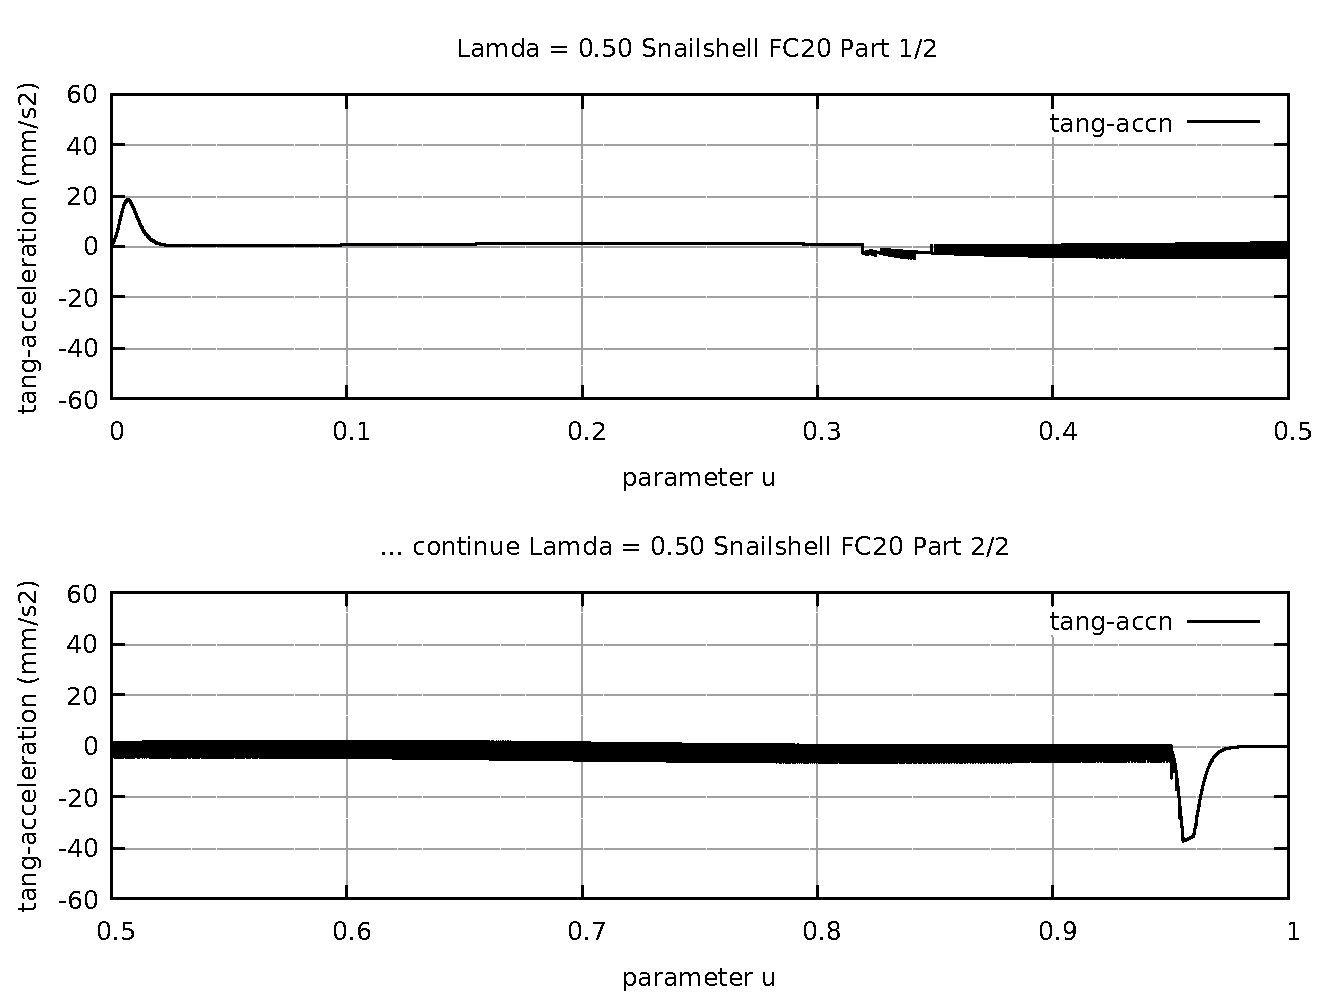
\includegraphics[width=1.30\textwidth]{Chap4/Lamda/jitters/Example-Snailshell-Jitters-Lamda-050-FC20-Part-1-of-2.pdf} 
	\end{figure}
\end{landscape}

%% ==================================
\clearpage
\pagebreak
\begin{landscape}
	\begin{figure}
		\centering
		\caption  {Example Snailshell Close View Tangential Acceleration Jitters}
		\label{img-Example Snailshell Close View Tangential Acceleration Jitters}
		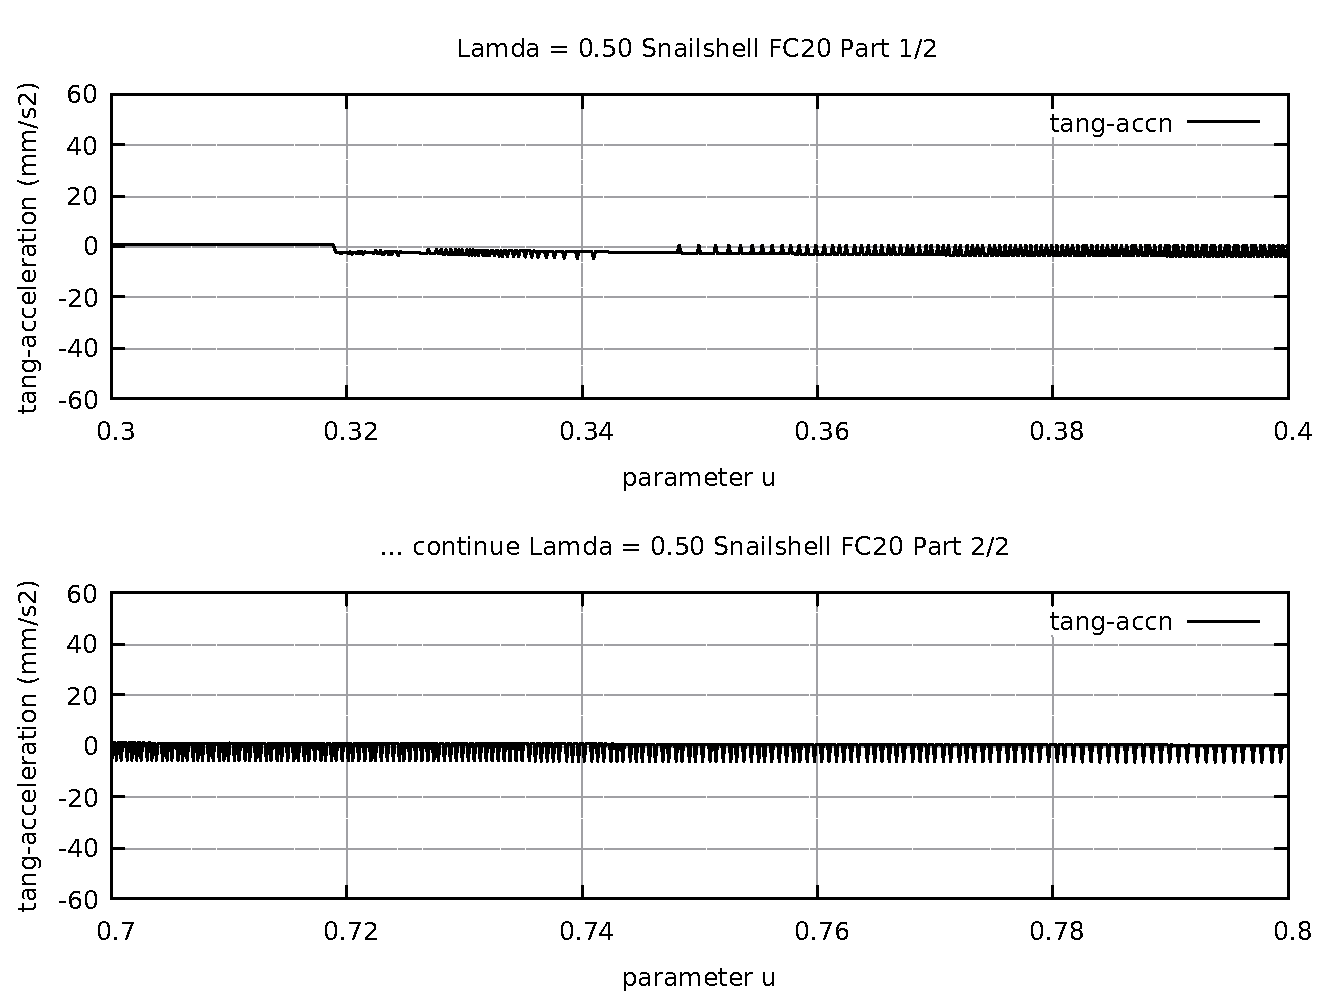
\includegraphics[width=1.30\textwidth]{Chap4/Lamda/jitters/Example-Snailshell-Jitters-Lamda-050-FC20-Part-2-of-2.pdf} 
	\end{figure}
\end{landscape}

%% ===================================
%% ==================================
\clearpage
\pagebreak
\begin{landscape}
	\begin{figure}
		\centering
		\caption  {Example Ribbon-100L Tangential Acceleration Jitters}
		\label{img-Example Ribbon-100L Tangential Acceleration Jitters}
		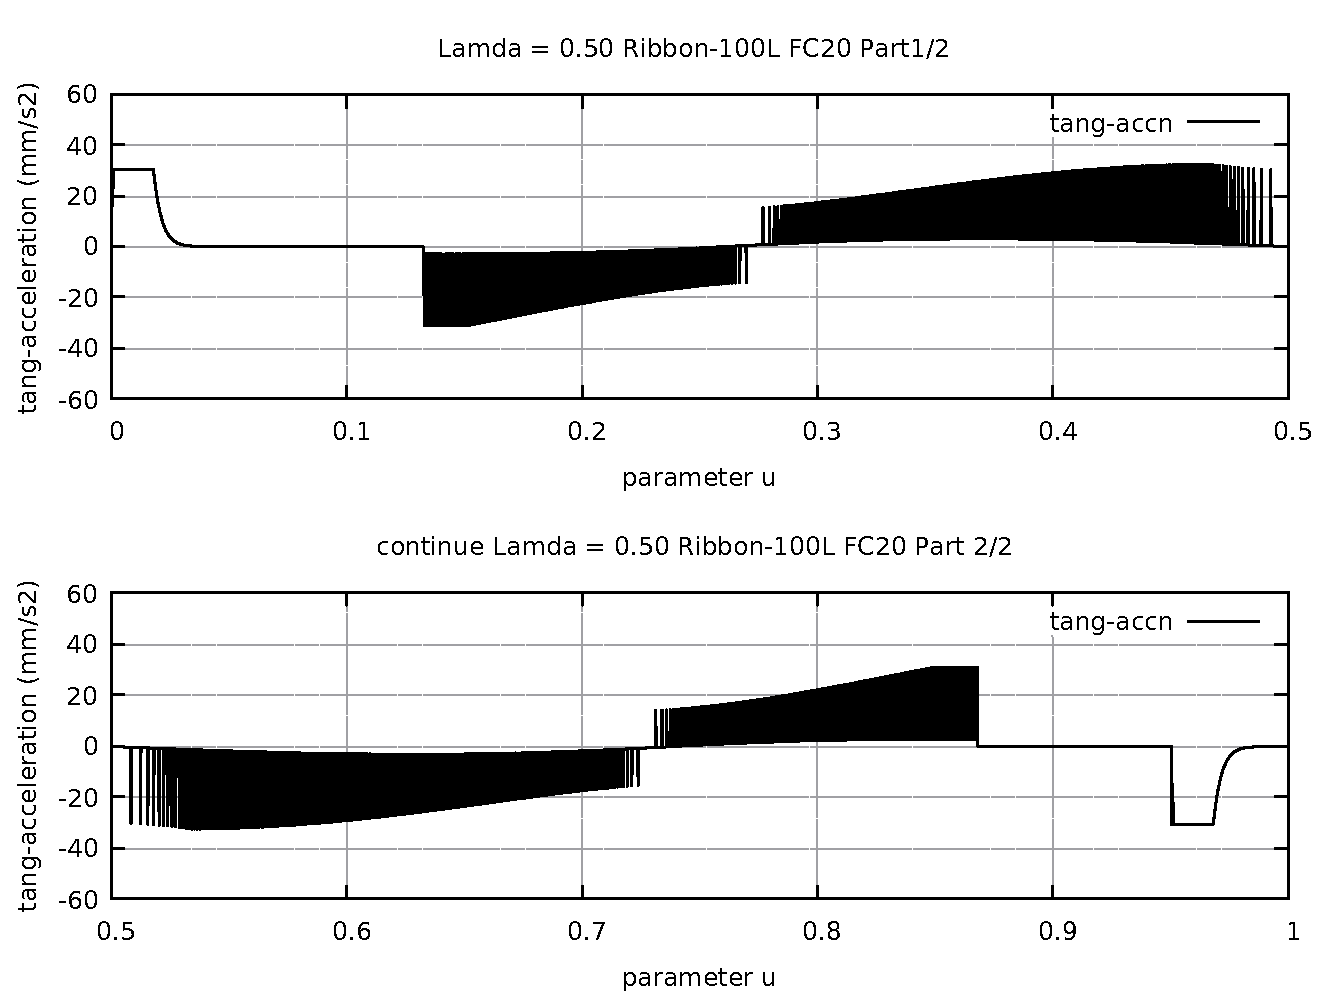
\includegraphics[width=1.30\textwidth]{Chap4/Lamda/jitters/Example-Ribbon-100L-Jitters-Lamda-050-FC20-Part-1-of-2.pdf} 
	\end{figure}
\end{landscape}

%% ==================================
\clearpage
\pagebreak
\begin{landscape}
	\begin{figure}
		\centering
		\caption  {Example Ribbon-100L Close View Tangential Acceleration Jitters}
		\label{img-Example Ribbon-100L Close View Tangential Acceleration Jitters}
		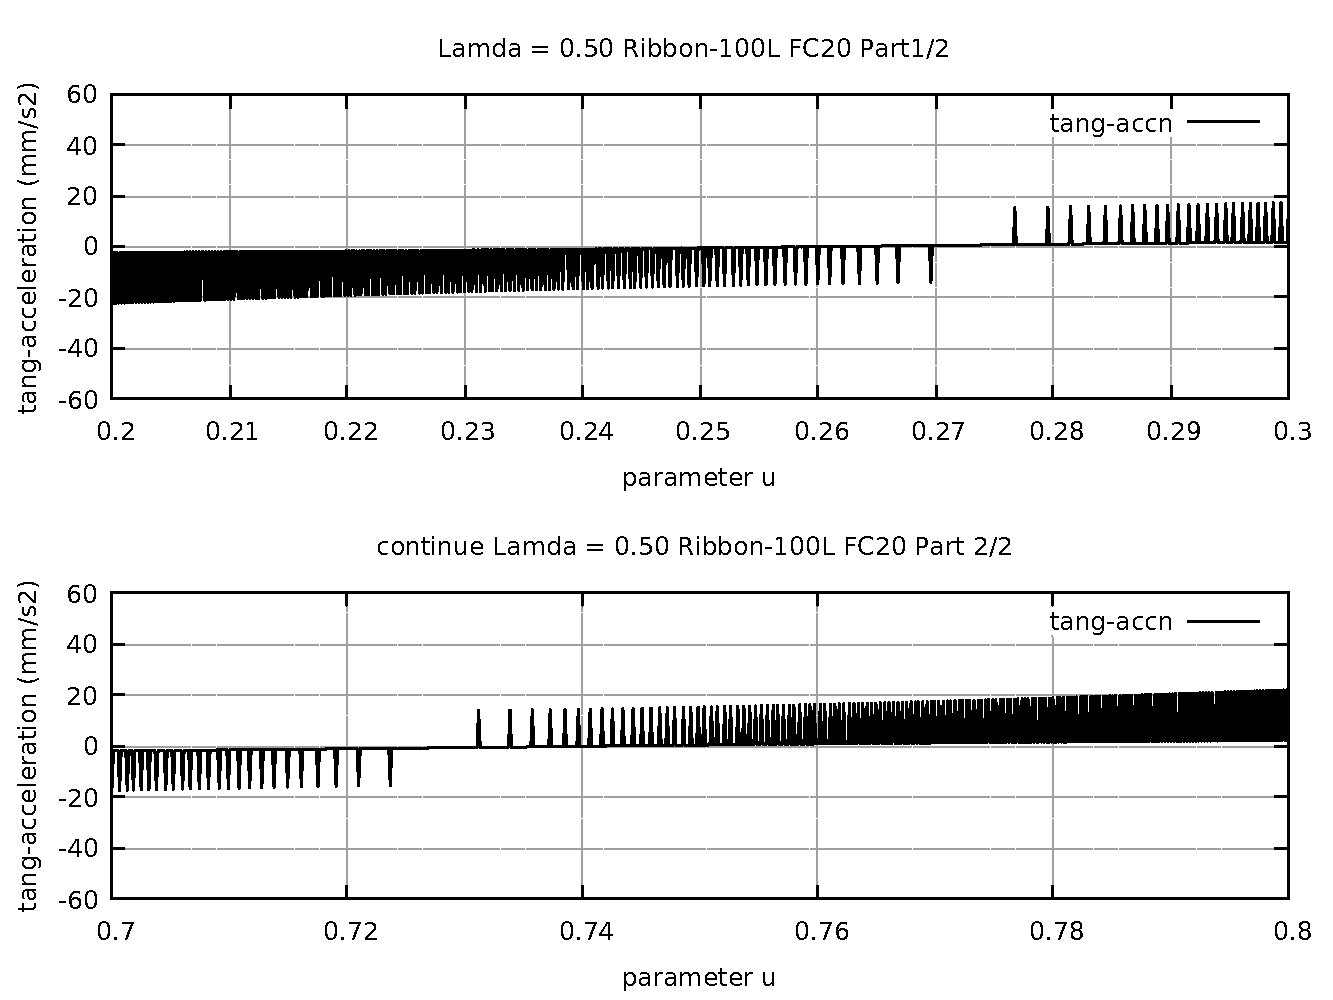
\includegraphics[width=1.30\textwidth]{Chap4/Lamda/jitters/Example-Ribbon-100L-Jitters-Lamda-050-FC20-Part-2-of-2.pdf} 
	\end{figure}
\end{landscape}

%% =================================================================
%% =================================================================
\clearpage
\pagebreak

\subsection{Results for finding acceptable lamda} \label{ssec-Results for finding acceptable lamda}

The next ten(10) pages of results contain the tangential acceleration profiles for all ten(10) parametric curves handled in this work. Each page contains four(4) plot executions for one particular curve at lamda = 0.10, 0.18, 0.20 and 0.50. All executions run at Feedrate Command FC = 20 mm/s. \\

On each page, lamda = 0.10 for the upper left plot, lamda = 0.18 for the lower left plot, lamda = 0.20 for the upper right plot, and lamda = 0.50 for the lower right plot. Attention must be made to lamda = 0.18 that is located at the lower left plot on the page. \\

\noindent
The list of parametric curves with tangential acceleration profiles are as follows.
	
\begin{table}[ht]
%% \begin{center}
\caption    {Results for finding acceptable lamda}
\label  {tab-Results for finding acceptable lamda}
	
%% IMPORTANT TO SCALEBOX BELOW
\scalebox{0.90}{
		
%% START COPY AND PASTE BELOW HERE
%% FROM \begin{tabular} UNTIL \end{tabular)
		
\begin{tabular}{ p{0.5cm} p{3.50cm} p{4.00cm} p{3.00cm} p{3.50cm} }
\hline
    &	        	 &                &                  	& 	\\
No. &	Curve Type	 & Reference Link & lamda = 0.18	& Remarks	\\
    &	        	 &                &                  	& 	\\
1	& Circle         & Figure [\ref{img-Circle Lamda Safety Factor Threshold}]         & good & \\
2	& Ellipse        & Figure [\ref{img-Ellipse Lamda Safety Factor Threshold}]        & good & \\
3	& Teardrop       & Figure [\ref{img-Teardrop Lamda Safety Factor Threshold}]       & good & lamda = 0.20 is bad\\
4	& Butterfly      & Figure [\ref{img-Butterfly Lamda Safety Factor Threshold}]      & suspect & To recheck\\
5	& Snailshell     & Figure [\ref{img-Snailshell Lamda Safety Factor Threshold}]     & good & \\
6	& Skewed-Astroid & Figure [\ref{img-Skewed-Astroid Lamda Safety Factor Threshold}] & good & \\
7	& Ribbon-10L     & Figure [\ref{img-Ribbon-10L Lamda Safety Factor Threshold}]     & good & \\
8	& Ribbon-100L    & Figure [\ref{img-Ribbon-100L Lamda Safety Factor Threshold}]    & good & \\
9	& AstEpi         & Figure [\ref{img-AstEpi Lamda Safety Factor Threshold}]         & good & \\
10	& SnaHyp         & Figure [\ref{img-SnaHyp Lamda Safety Factor Threshold}]         & suspect & To recheck\\
    &	        	 &                &                  	& 	
\end{tabular}

%% END COPY AND PASTE		

}   %% IMPORTANT FOR SCALEBOX CLOSING
\hrule
\end{table}


\noindent
For those curves that the lamda = 0.18 is suspect, a close inspection for jitters is required. All plots in the next pages are in landscape mode.\\

%% =================================================================
\clearpage
\pagebreak

\subsection{Rechecking acceptable lamda}

\noindent
Close inspection for the following two(2) curves both at lamda = 0.18, Butterfly and SnaHyp revealed the following.

\begin{table}[ht]
%% \begin{center}
\caption    {Results for rechecking acceptable lamda}
\label  {tab-Results for rechecking acceptable lamda}
	
%% IMPORTANT TO SCALEBOX BELOW
\scalebox{0.90}{
		
%% START COPY AND PASTE BELOW HERE
%% FROM \begin{tabular} UNTIL \end{tabular)
		
\begin{tabular}{ p{0.5cm} p{3.50cm} p{4.00cm} p{3.00cm} p{3.50cm} }
\hline
    &	        	 &                &                 & 	\\
No. &	Curve Type	 & Reference Link & lamda = 0.18	& Remarks	\\
	&	        	 &                &                 & 	\\
4A	& Butterfly      & Figure [\ref{img-Butterfly Tangential Acceleration Magnified 2X}] & good & 2X magnification\\
4B	& Butterfly      & Figure [\ref{img-Butterfly Tangential Acceleration Closeup View}] & good & Close up view\\
10A	& SnaHyp         & Figure [\ref{img-SnaHyp Tangential Acceleration Magnified 2X}]    & good & 2X magnification\\
10B	& SnaHyp         & Figure [\ref{img-SnaHyp Tangential Acceleration Closeup View}]    & good & Close up view\\
&	        	 &                &                  	& 	
\end{tabular}
		
%% END COPY AND PASTE		
		
}   %% IMPORTANT FOR SCALEBOX CLOSING
\hrule
\end{table}

\noindent
In conclusion, lamda = 0.18 is the acceptable acceleration safety factor to be applied in the execution of all ten(10) parametric curves.\\
 
%% ==================================
\clearpage
\pagebreak
\begin{landscape}
\begin{figure}
\centering
\caption  {Circle Lamda Safety Factor Threshold}
\label{img-Circle Lamda Safety Factor Threshold}
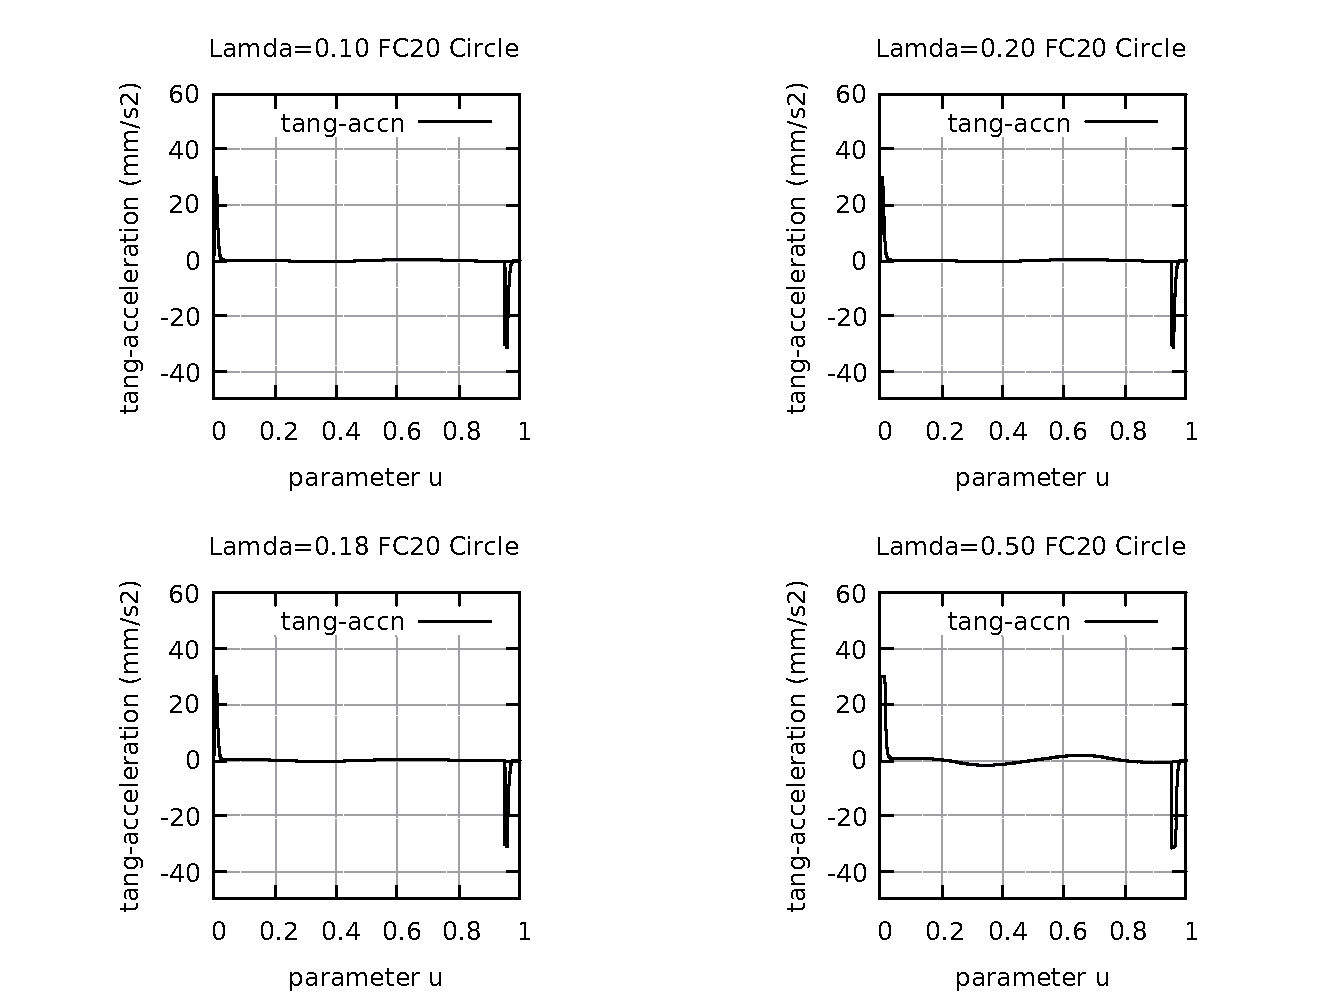
\includegraphics[width=1.30\textwidth]{Chap4/Lamda/img-4plots-CIRCLE-Lamda-010-018-020-050-FC20-Tang-Accn.pdf} 
\end{figure}
\end{landscape}


%% ==================================
\clearpage
\pagebreak
\begin{landscape}
	\begin{figure}
		\centering
		\caption  {Ellipse Lamda Safety Factor Threshold}
		\label{img-Ellipse Lamda Safety Factor Threshold}
		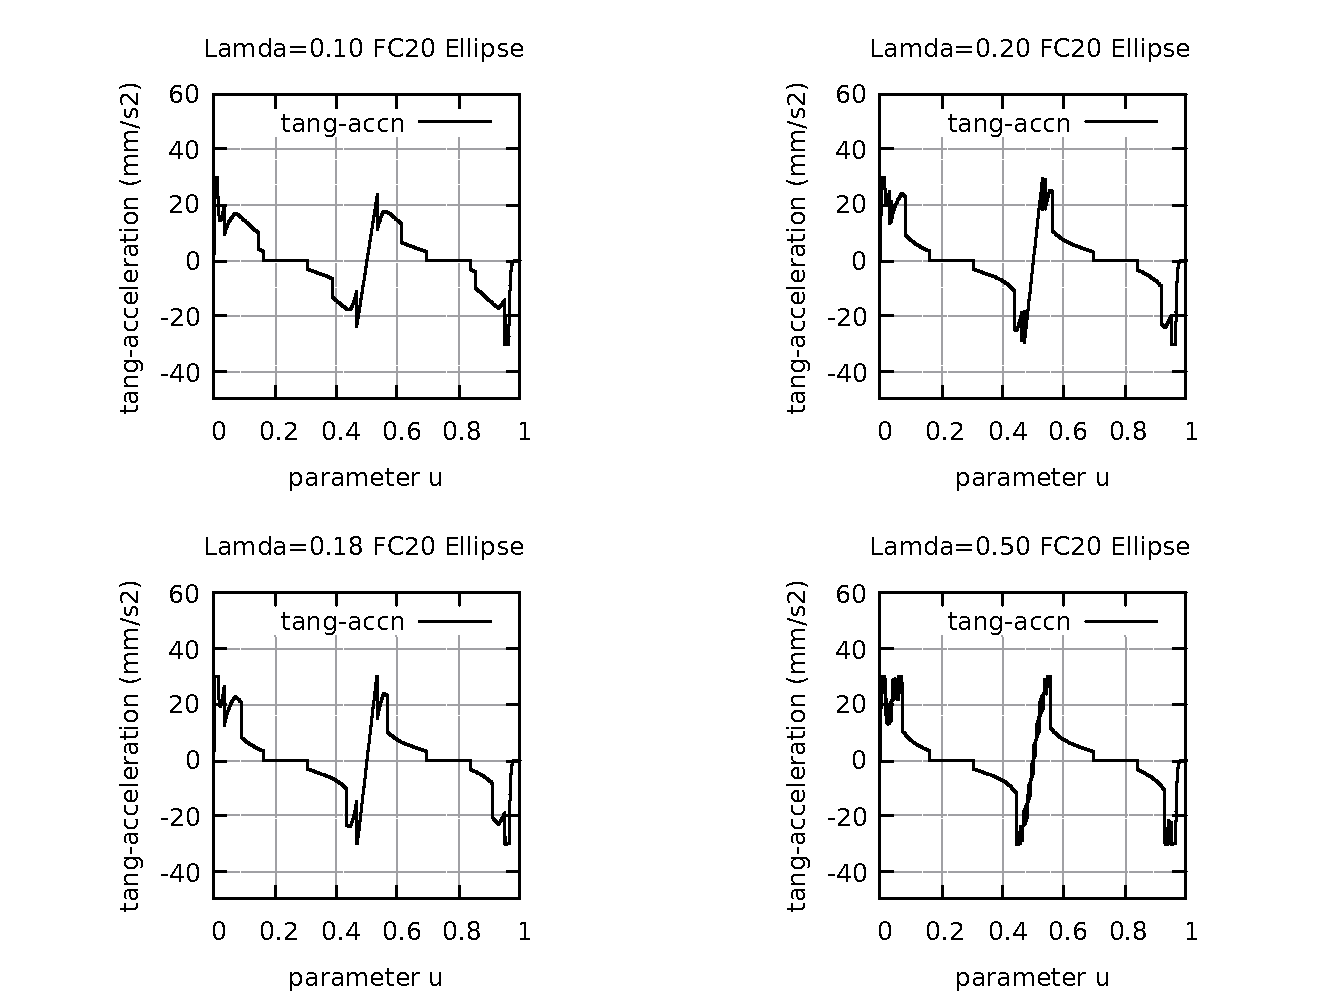
\includegraphics[width=1.30\textwidth]{Chap4/Lamda/img-4plots-ELLIPSE-Lamda-010-018-020-050-FC20-Tang-Accn.pdf} 
	\end{figure}
\end{landscape}

%% ==================================
\clearpage
\pagebreak
\begin{landscape}
	\begin{figure}
		\centering
		\caption  {Teardrop Lamda Safety Factor Threshold}
		\label{img-Teardrop Lamda Safety Factor Threshold}
		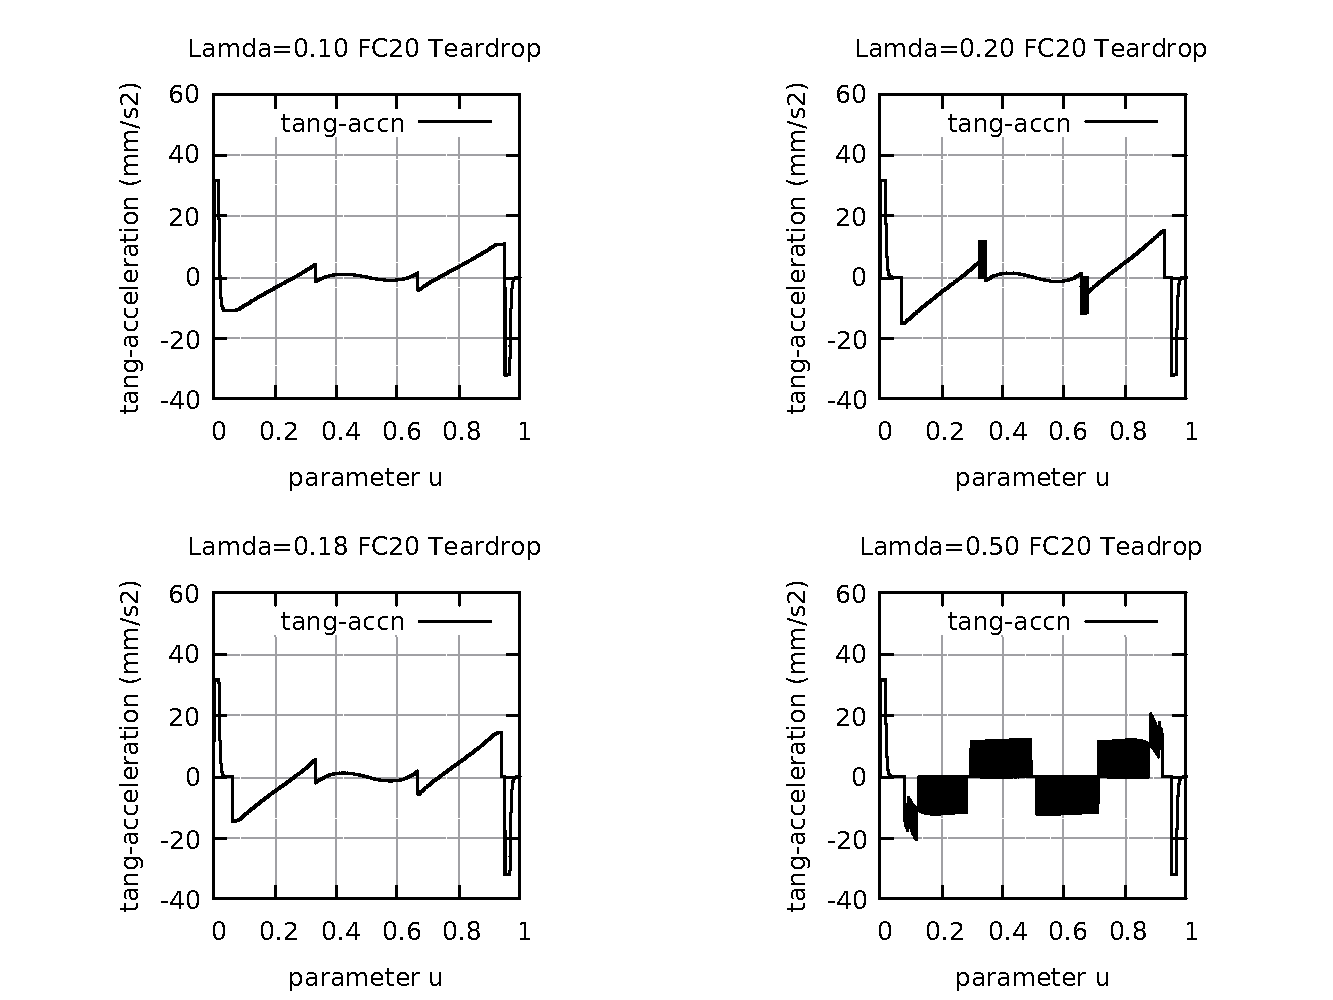
\includegraphics[width=1.30\textwidth]{Chap4/Lamda/img-4plots-TEARDROP-Lamda-010-018-020-050-FC20-Tang-Accn.pdf} 
	\end{figure}
\end{landscape}

%% ==================================
\clearpage
\pagebreak
\begin{landscape}
	\begin{figure}
		\centering
		\caption  {Butterfly Lamda Safety Factor Threshold}
		\label{img-Butterfly Lamda Safety Factor Threshold}
		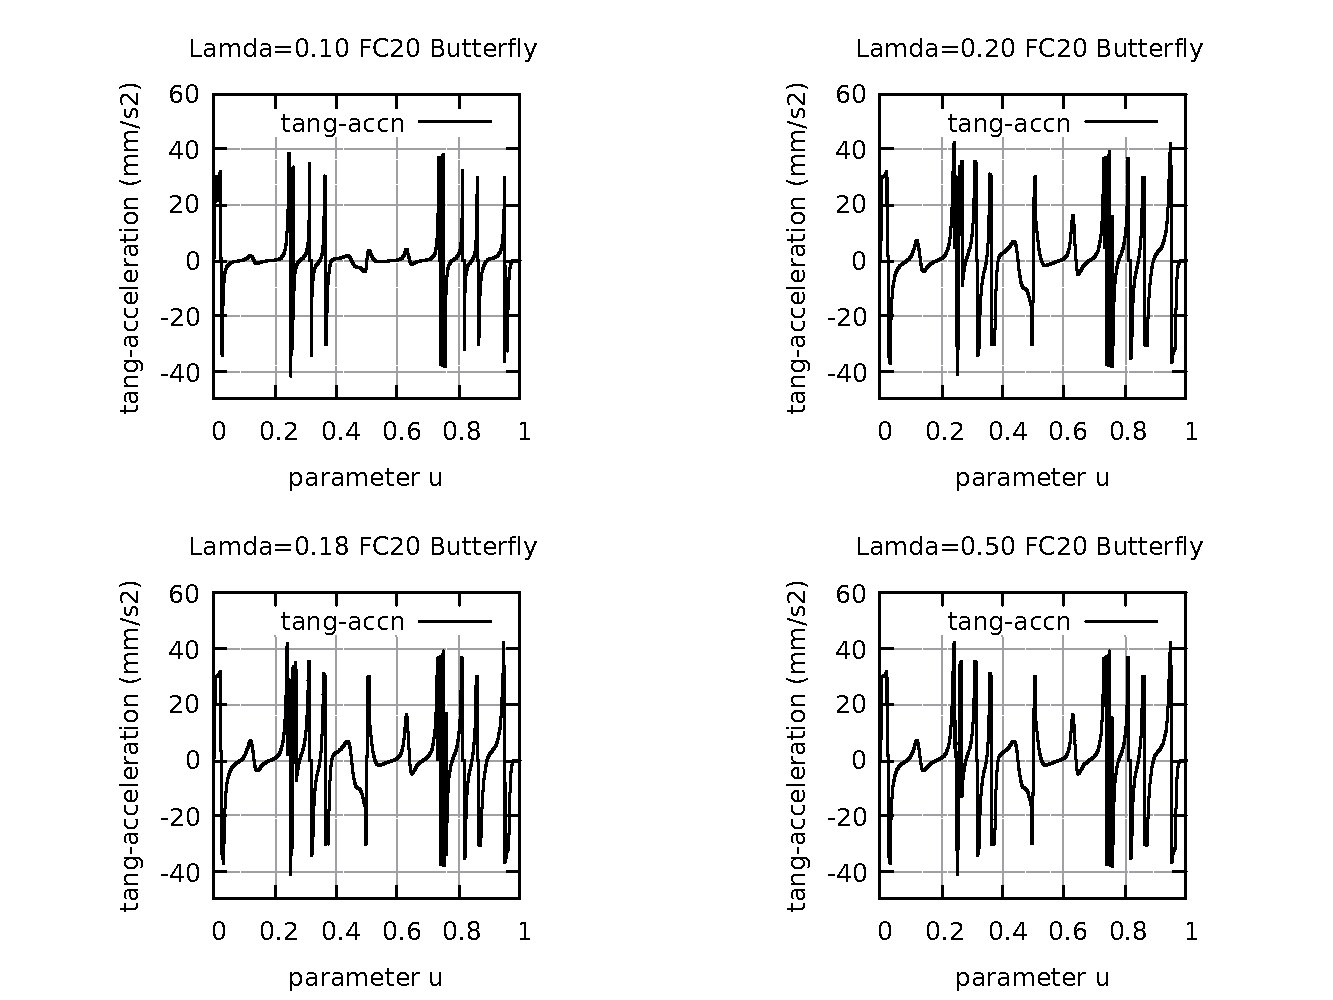
\includegraphics[width=1.30\textwidth]{Chap4/Lamda/img-4plots-BUTTERFLY-Lamda-010-018-020-050-FC20-Tang-Accn.pdf} 
	\end{figure}
\end{landscape}

%% ==================================
\clearpage
\pagebreak
\begin{landscape}
	\begin{figure}
		\centering
		\caption  {Snailshell Lamda Safety Factor Threshold}
		\label{img-Snailshell Lamda Safety Factor Threshold}
		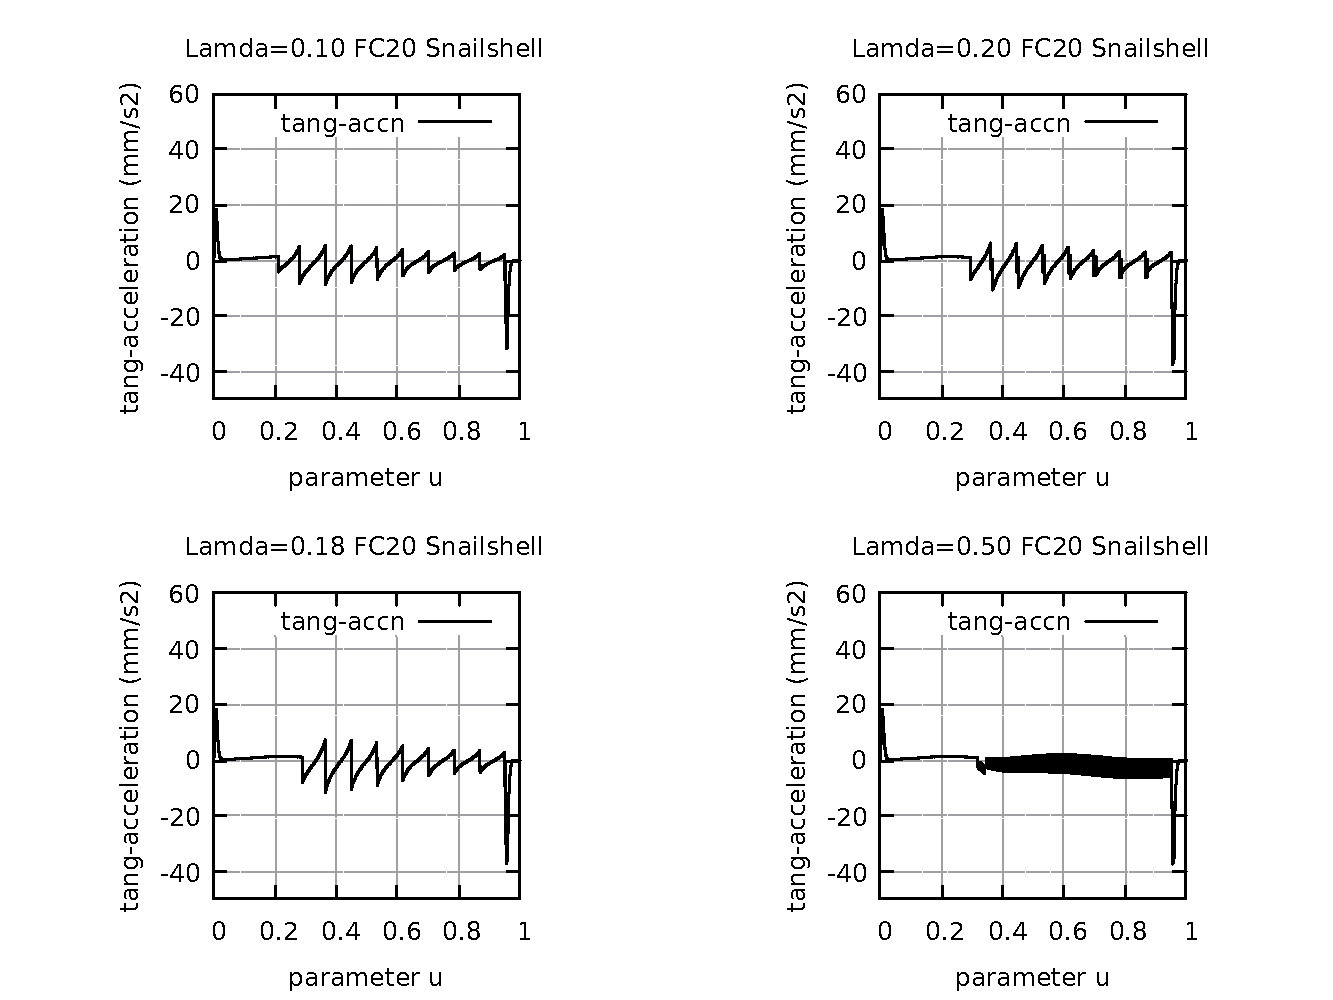
\includegraphics[width=1.30\textwidth]{Chap4/Lamda/img-4plots-SNAILSHELL-Lamda-010-018-020-050-FC20-Tang-Accn.pdf} 
	\end{figure}
\end{landscape}

%% ==================================
%% ==================================
\clearpage
\pagebreak
\begin{landscape}
	\begin{figure}
		\centering
		\caption  {Skewed-Astroid Lamda Safety Factor Threshold}
		\label{img-Skewed-Astroid Lamda Safety Factor Threshold}
		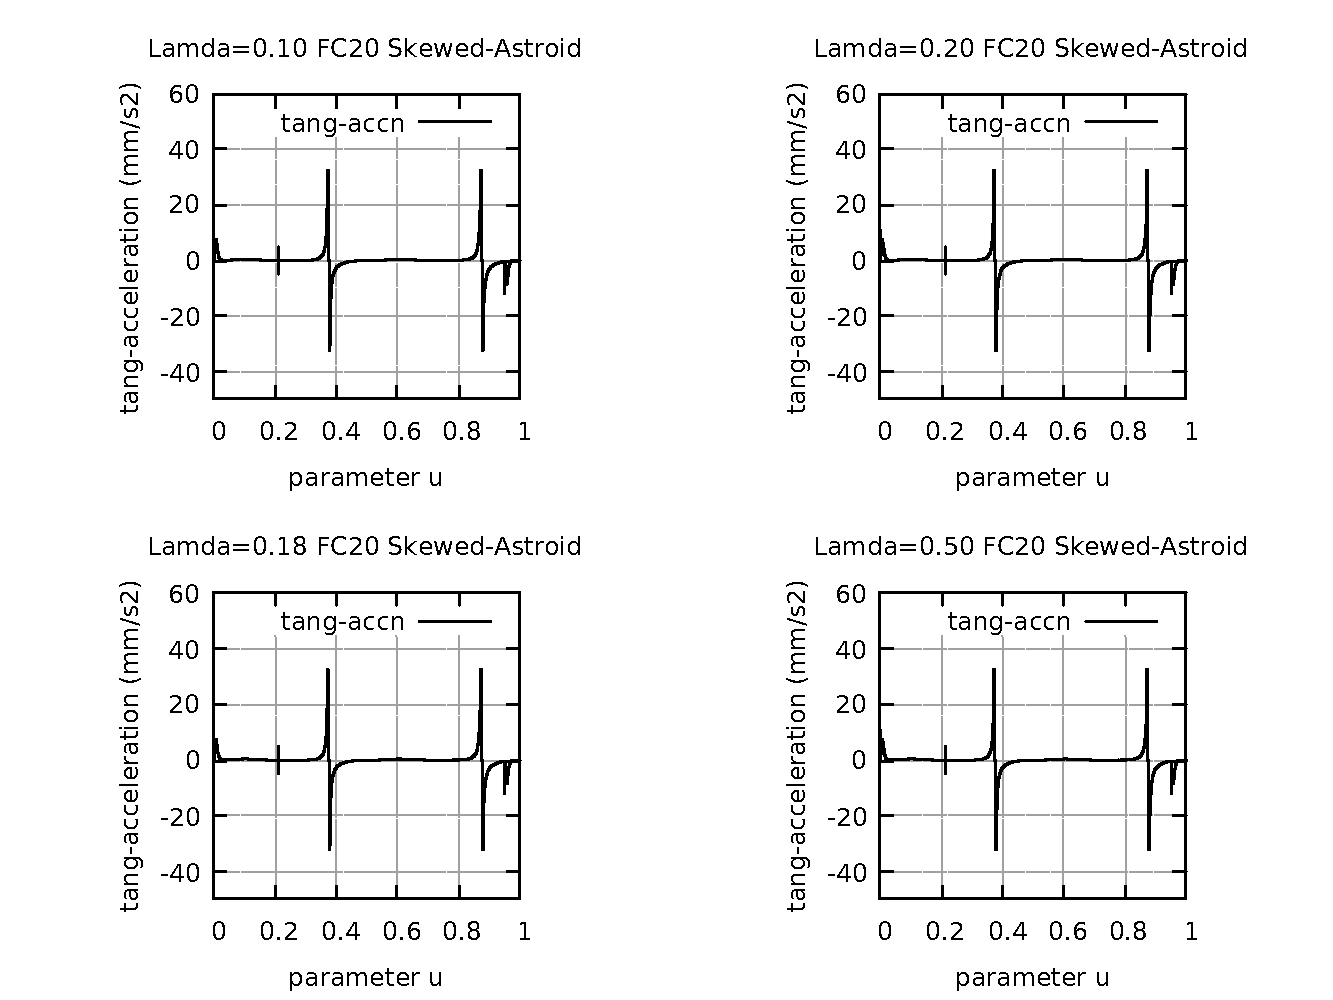
\includegraphics[width=1.30\textwidth]{Chap4/Lamda/img-4plots-SKEWED-ASTROID-Lamda-010-018-020-050-FC20-Tang-Accn.pdf} 
	\end{figure}
\end{landscape}


%% ==================================
\clearpage
\pagebreak
\begin{landscape}
	\begin{figure}
		\centering
		\caption  {Ribbon-10L Lamda Safety Factor Threshold}
		\label{img-Ribbon-10L Lamda Safety Factor Threshold}
		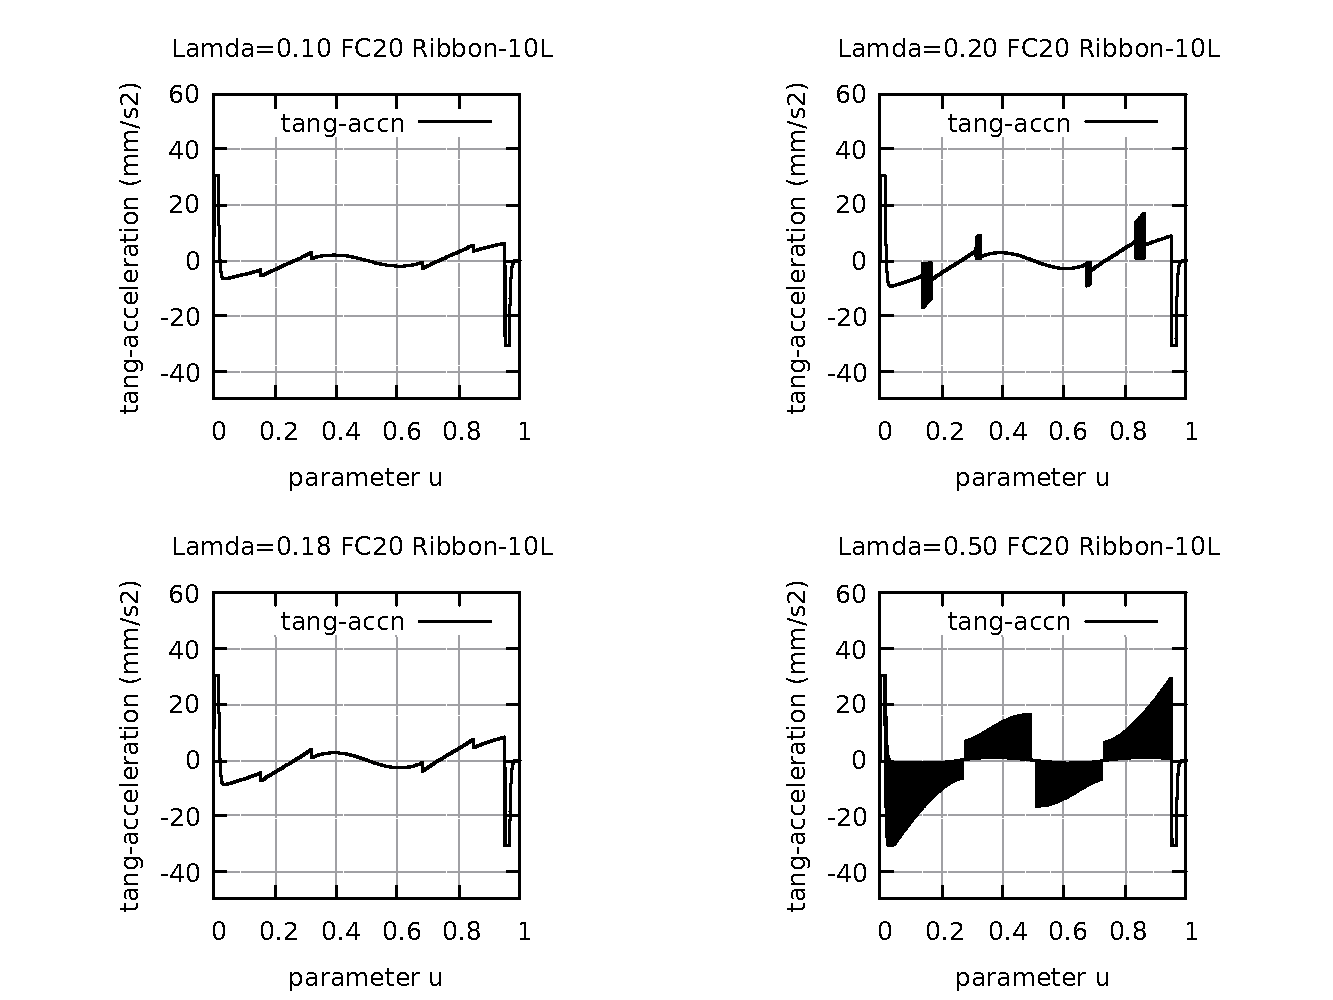
\includegraphics[width=1.30\textwidth]{Chap4/Lamda/img-4plots-RIBBON-10L-Lamda-010-018-020-050-FC20-Tang-Accn.pdf} 
	\end{figure}
\end{landscape}

%% ==================================
\clearpage
\pagebreak
\begin{landscape}
	\begin{figure}
		\centering
		\caption  {Ribbon-100L Lamda Safety Factor Threshold}
		\label{img-Ribbon-100L Lamda Safety Factor Threshold}
		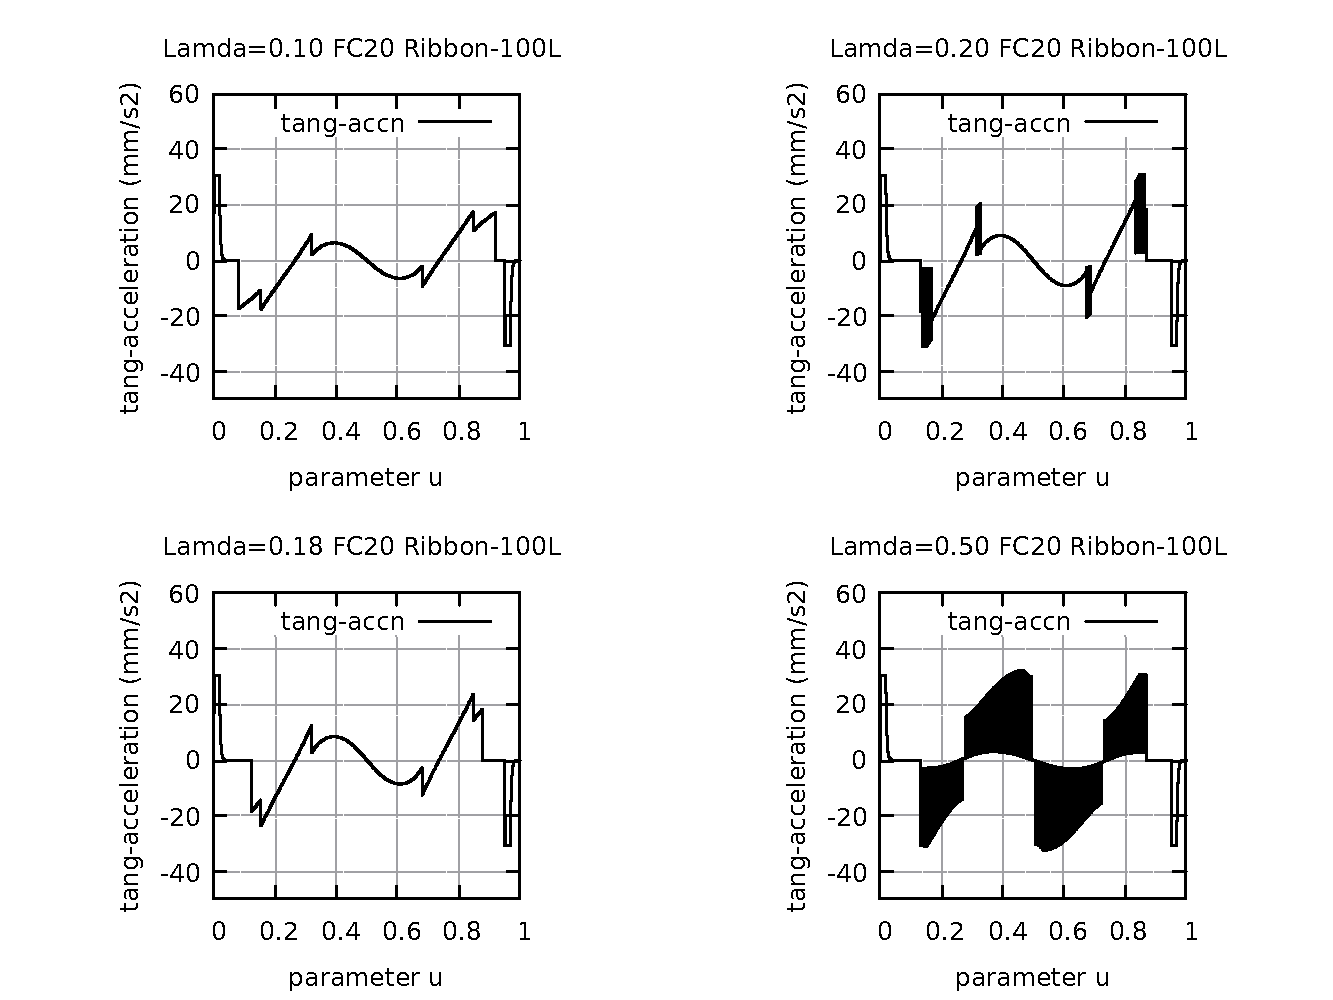
\includegraphics[width=1.30\textwidth]{Chap4/Lamda/img-4plots-RIBBON-100L-Lamda-010-018-020-050-FC20-Tang-Accn.pdf} 
	\end{figure}
\end{landscape}

%% ==================================
\clearpage
\pagebreak
\begin{landscape}
	\begin{figure}
		\centering
		\caption  {AstEpi Lamda Safety Factor Threshold}
		\label{img-AstEpi Lamda Safety Factor Threshold}
		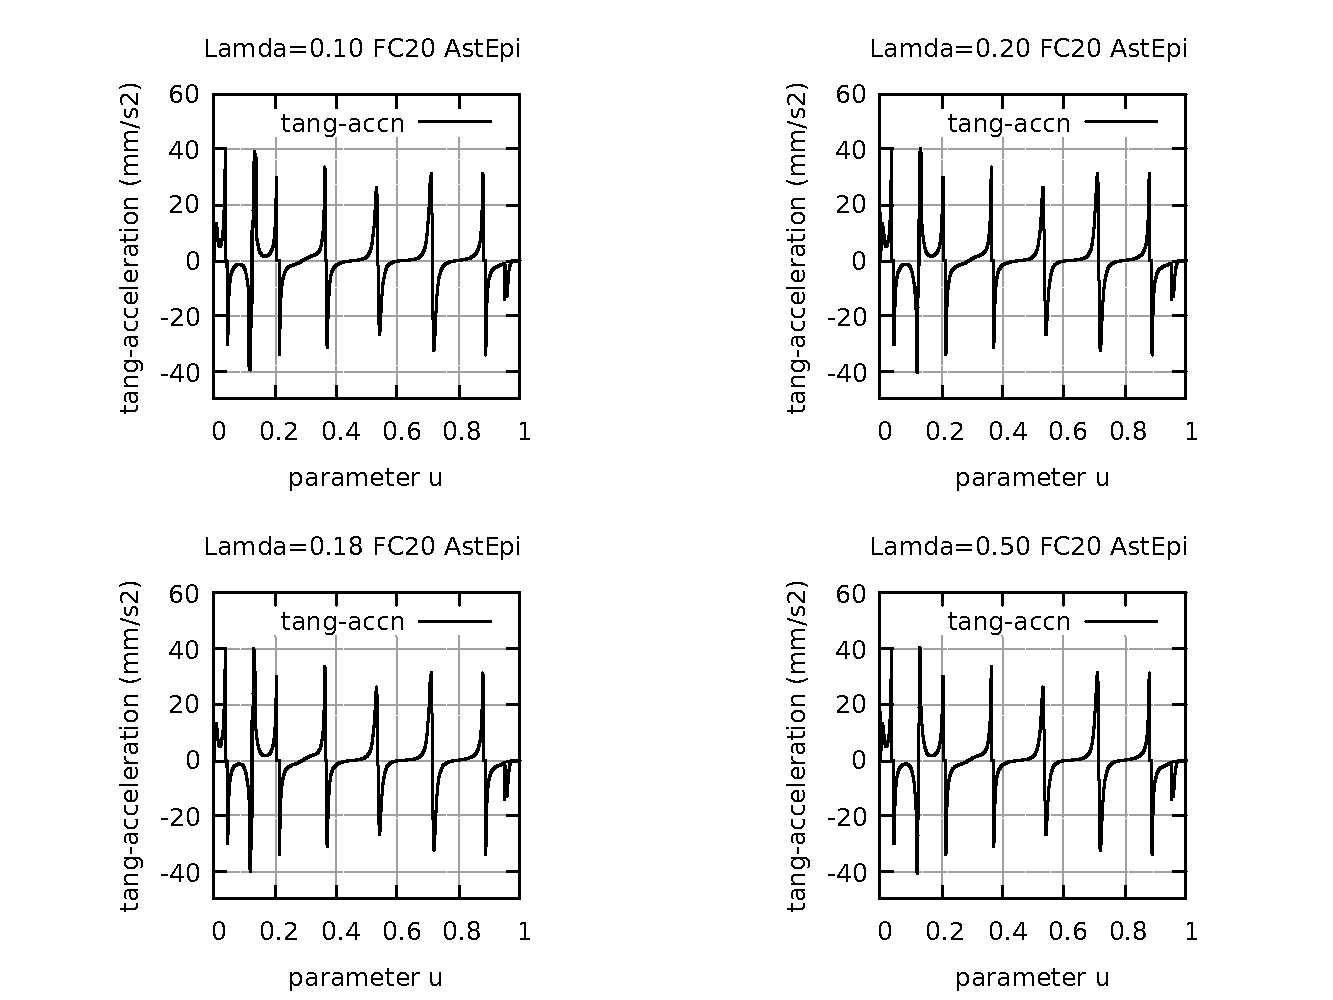
\includegraphics[width=1.30\textwidth]{Chap4/Lamda/img-4plots-ASTEPI-Lamda-010-018-020-050-FC20-Tang-Accn.pdf} 
	\end{figure}
\end{landscape}

%% ==================================
\clearpage
\pagebreak
\begin{landscape}
	\begin{figure}
		\centering
		\caption  {SnaHyp Lamda Safety Factor Threshold}
		\label{img-SnaHyp Lamda Safety Factor Threshold}
		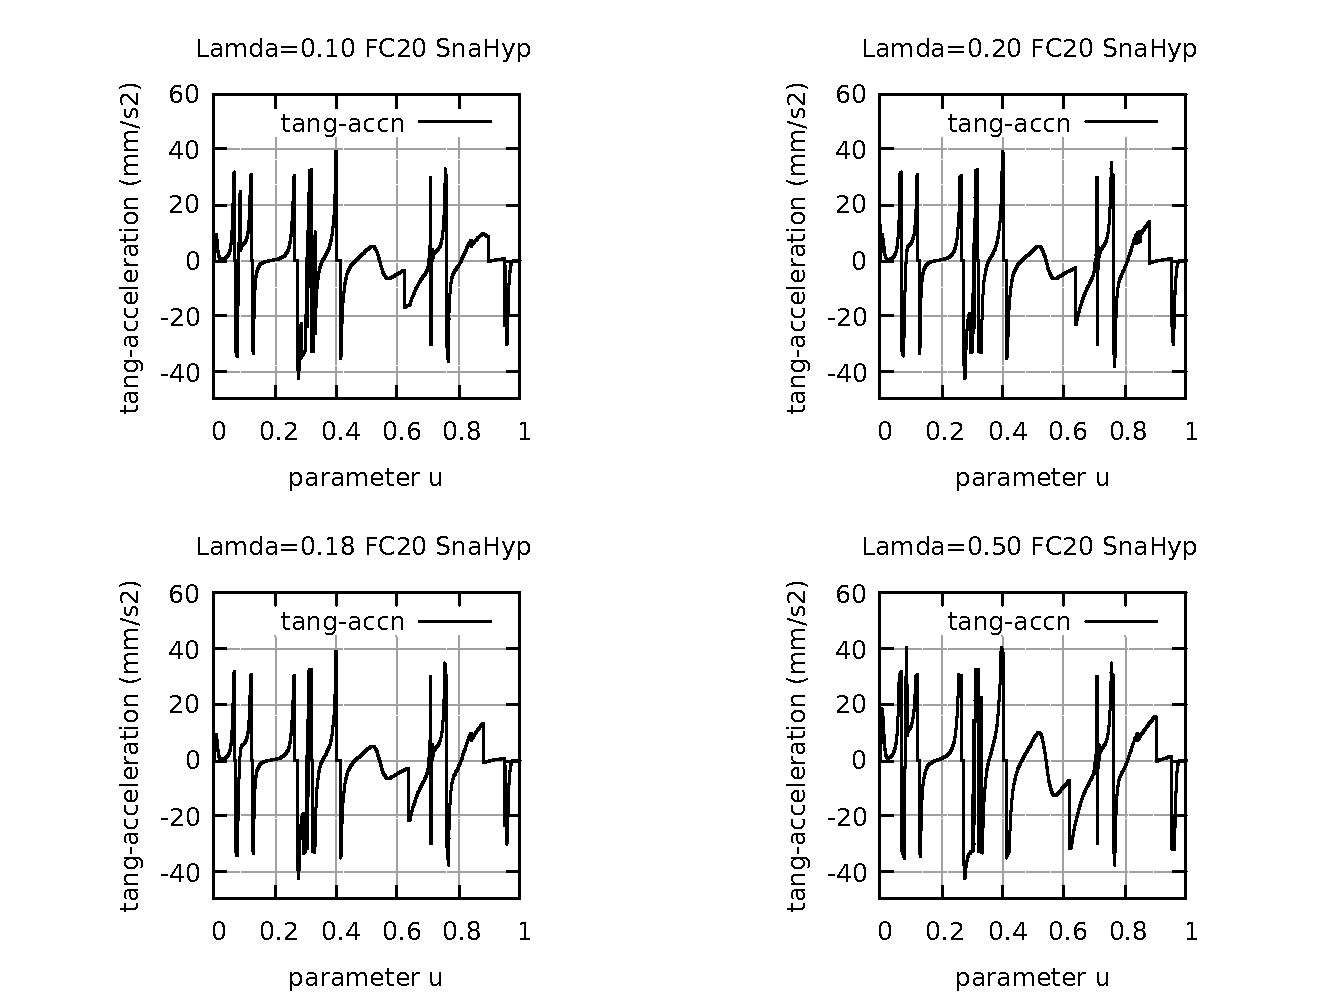
\includegraphics[width=1.30\textwidth]{Chap4/Lamda/img-4plots-SNAHYP-Lamda-010-018-020-050-FC20-Tang-Accn.pdf} 
	\end{figure}
\end{landscape}



%% =============================================================
%% =============================================================
\clearpage
\pagebreak
\begin{landscape}
	\begin{figure}
		\centering
		\caption  {Butterfly Tangential Acceleration Magnified 2X}
		\label{img-Butterfly Tangential Acceleration Magnified 2X}
		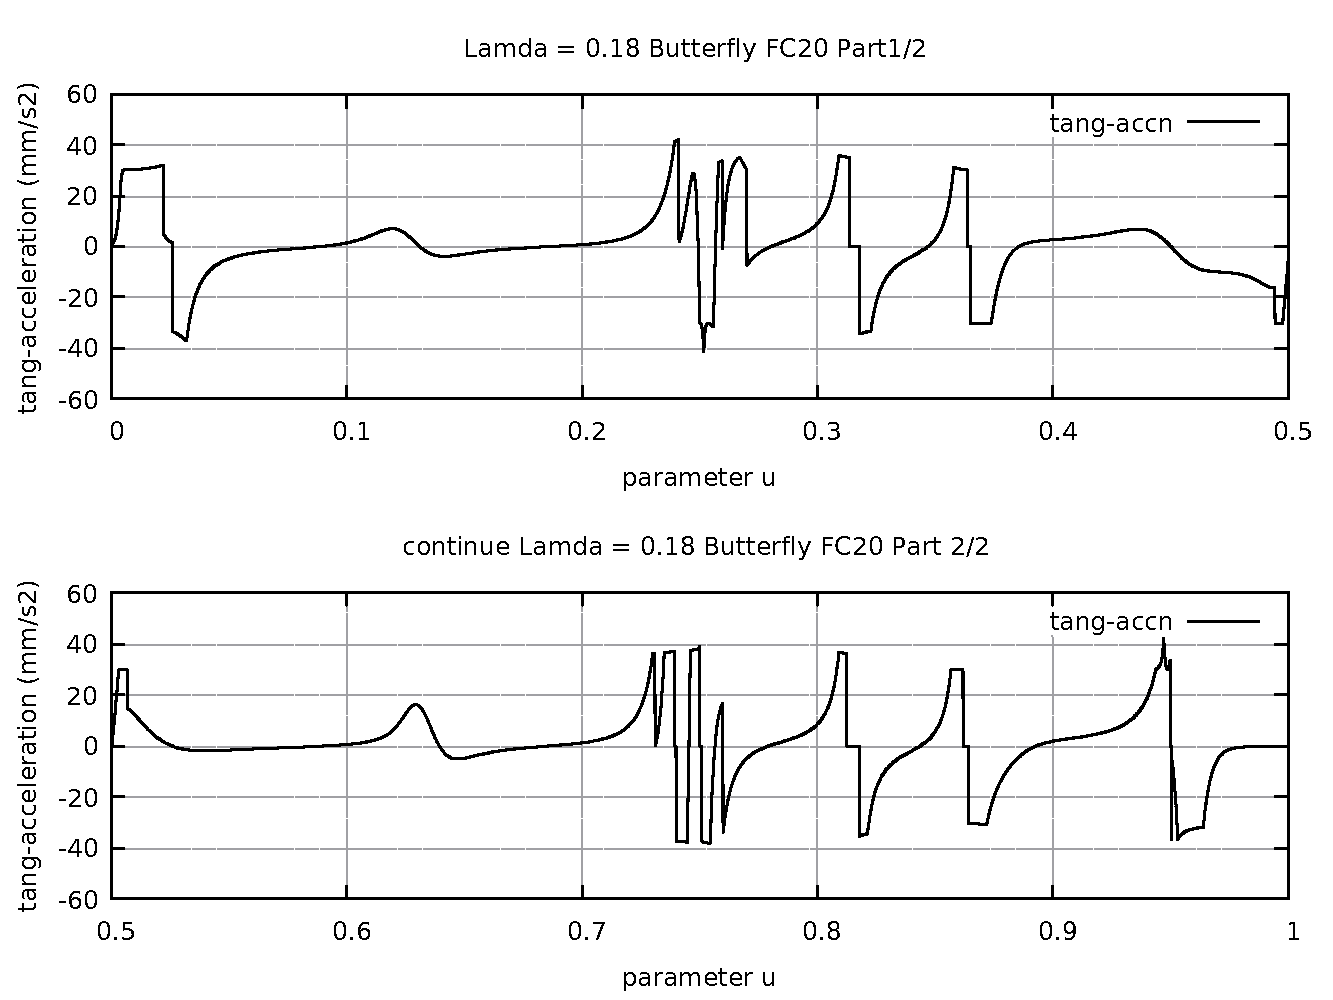
\includegraphics[width=1.30\textwidth]{Chap4/Lamda/magnify/Butterfly-Tang-Accn-Lamda-magnified-01.pdf} 
	\end{figure}
\end{landscape}

%% ==================================
\clearpage
\pagebreak
\begin{landscape}
	\begin{figure}
		\centering
		\caption  {Butterfly Tangential Acceleration Closeup View}
		\label{img-Butterfly Tangential Acceleration Closeup View}
		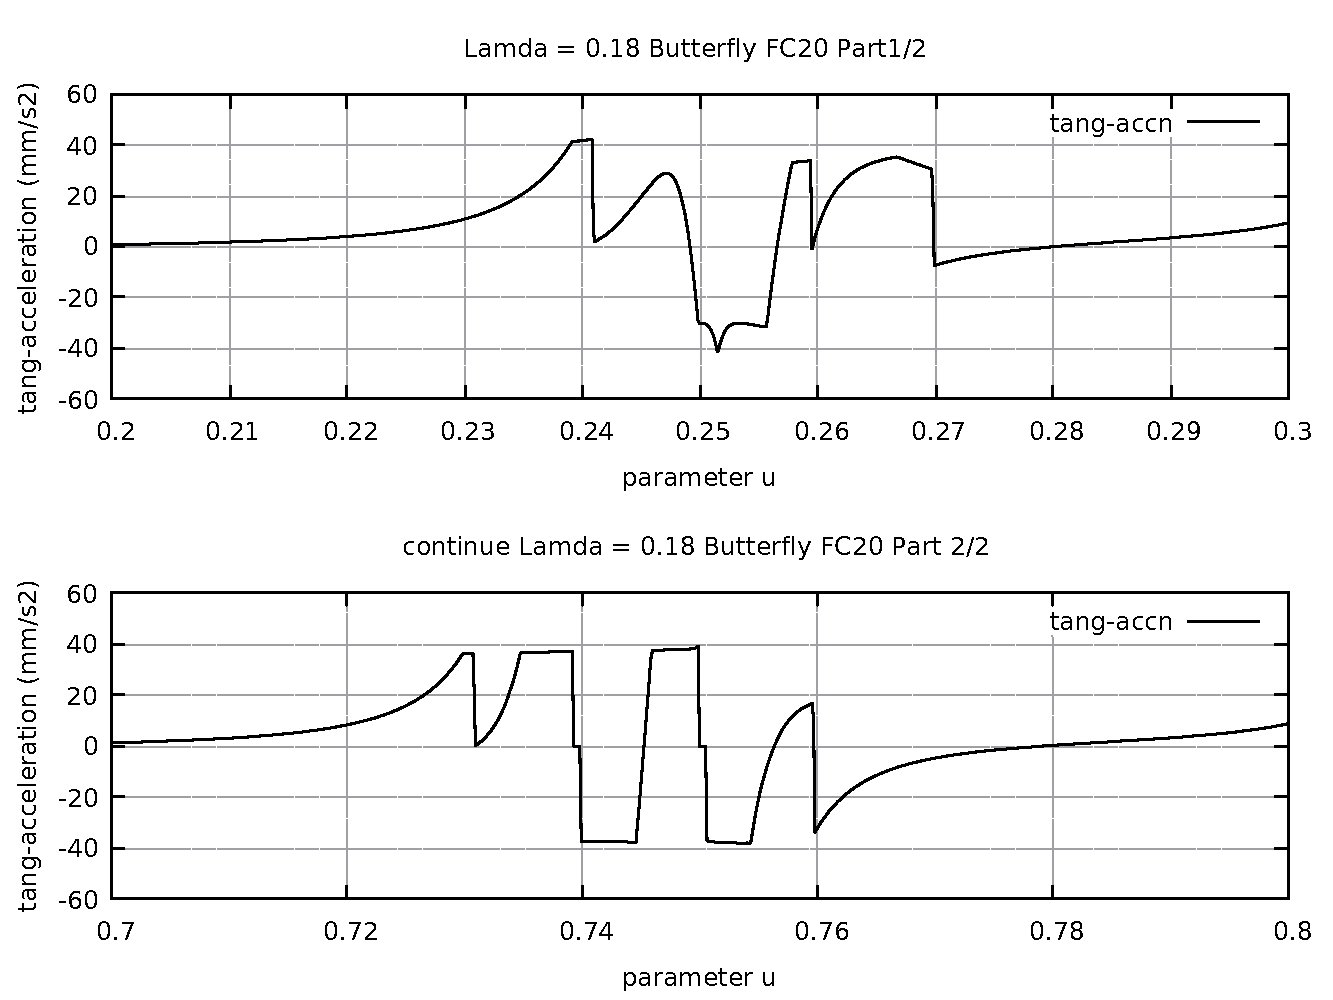
\includegraphics[width=1.30\textwidth]{Chap4/Lamda/magnify/Butterfly-Tang-Accn-Lamda-magnified-02.pdf} 
	\end{figure}
\end{landscape}

%% ===================================
%% ==================================
\clearpage
\pagebreak
\begin{landscape}
	\begin{figure}
		\centering
		\caption  {SnaHyp Tangential Acceleration Magnified 2X}
		\label{img-SnaHyp Tangential Acceleration Magnified 2X}
		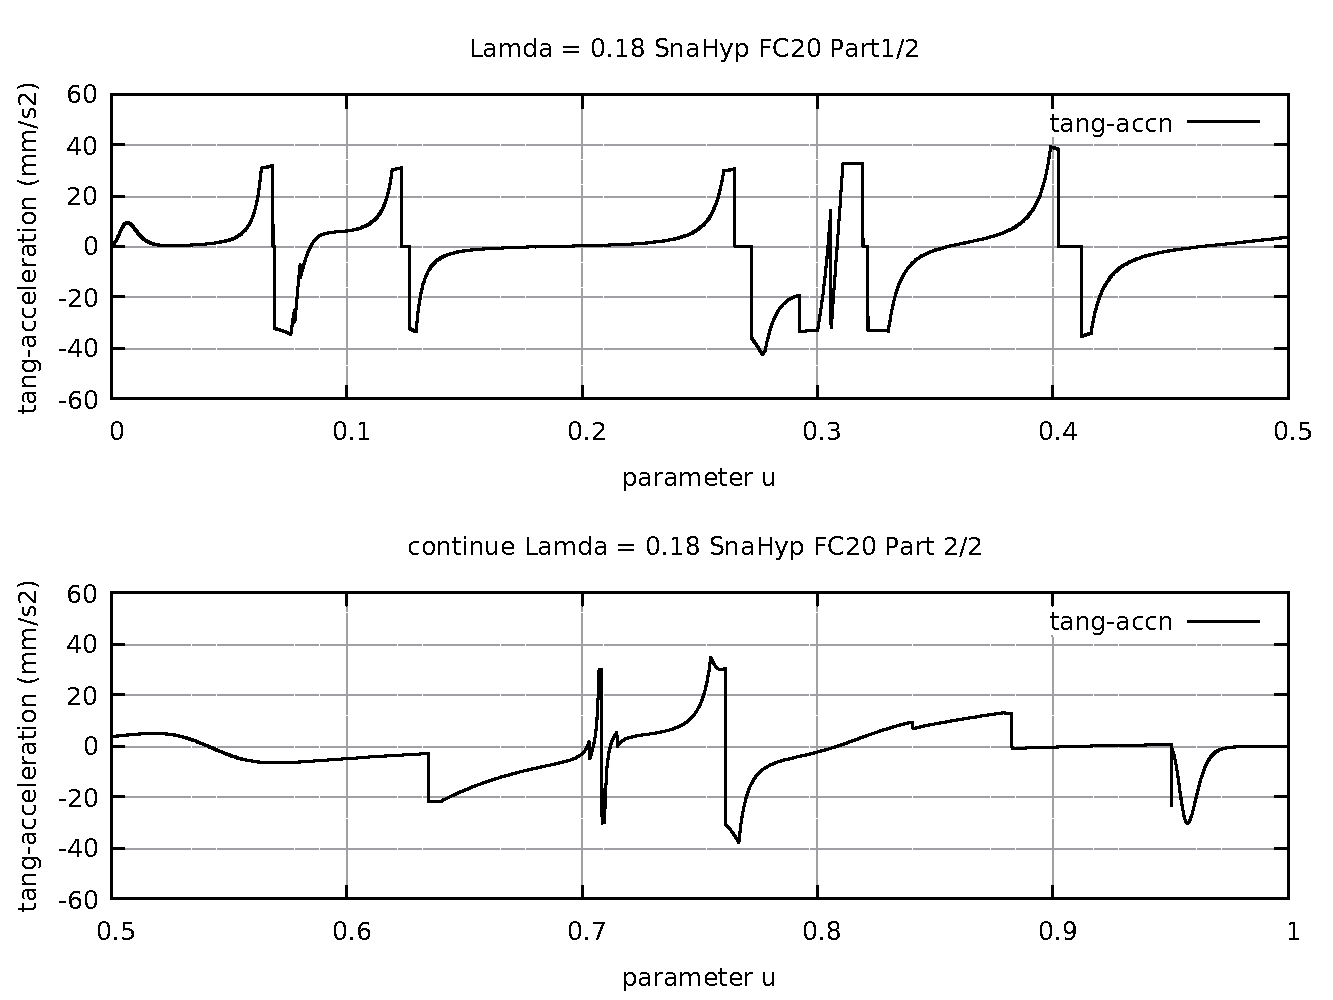
\includegraphics[width=1.30\textwidth]{Chap4/Lamda/magnify/SnaHyp-Tang-Accn-Lamda-magnified-01.pdf} 
	\end{figure}
\end{landscape}

%% ==================================
\clearpage
\pagebreak
\begin{landscape}
	\begin{figure}
		\centering
		\caption  {SnaHyp Tangential Acceleration Closeup View}
		\label{img-SnaHyp Tangential Acceleration Closeup View}
		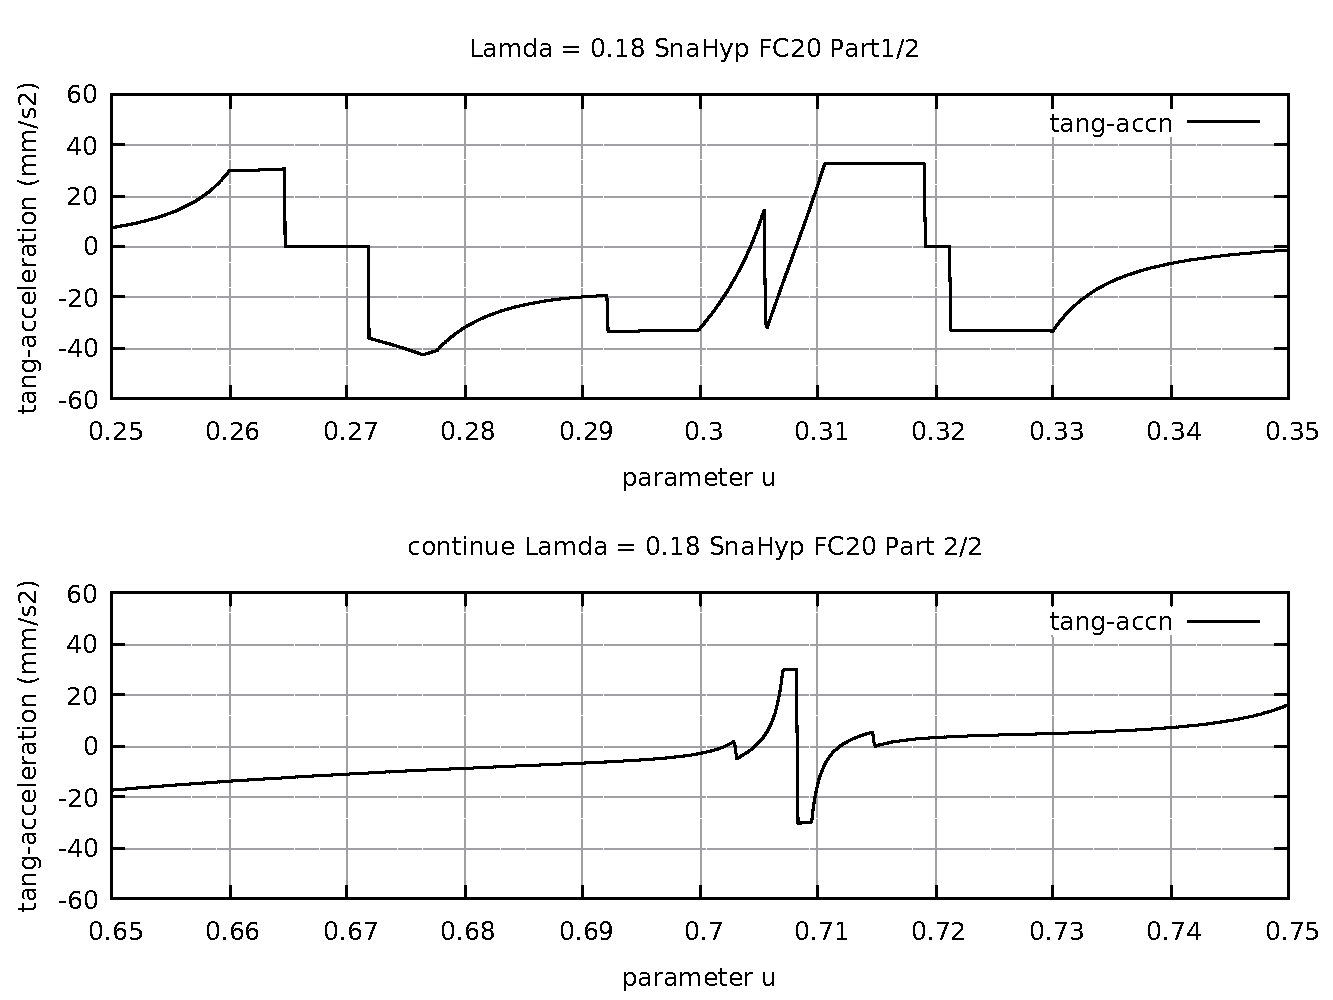
\includegraphics[width=1.30\textwidth]{Chap4/Lamda/magnify/SnaHyp-Tang-Accn-Lamda-magnified-02.pdf} 
	\end{figure}
\end{landscape}


%% =============================================================
%% ============================================================  
\clearpage
\pagebreak
\section{TEARDROP CURVE FOR ILLUSTRATION}
\label{chap4-TEARDROP CURVE FOR ILLUSTRATION}

\subsection{Teardrop parametric curve}

Instead of displaying the execution results of all ten(10) parametric curves in this chapter, only the full results of the Teardrop curve shall be displayed for illustration. The results for the rest of the parametric curves are provided in individual appendices specific to the corresponding curve. \\

The Teardrop curve was used as an illustrative example due to its special characteristics. It has the combination of all curve features studied in this work. The Teardrop curve contains, for example, gentle convex turns, near straight line sections, a sharp pointed apex akin to a cusp at the origin, a closed loop curve, symmetrical about the y-axis reflection but non-symmetrical about the x-axis reflection, and overall curve is not origin centered.    

\subsection{Rest of other nine(9) parametric curves} 
\label{chap4-Rest of nine parametric curves} 

The rest of the other curves studied in this work are essentially extreme variations of the Teardrop curve.

\begin{enumerate}
	\item \textbf{Circle in Appendix Reference} [App\ref{APPENDIX CIRCLE CURVE}]. \\
	The Circle curve was selected primarily to prove that the algorithm is performing correctly. For the Circle, the calculation of circumference by the standard geometry formula ($C = 2*PI*Radius$) can be validated and verified by comparing to the results of the algorithm for the total sum-arc-length and the total sum-chord-length, respectively. Since the circle spans a central angle of (2*PI) radians or 360 degrees, the results for the total sum-arc-theta calculated by the algorithm is another worthy comparison. To add challenge the interpolation algorithm, the radius of the circle was chosen to be 79, a prime number divisible only by one and itself. In this work, the Circle curve is therefore featurefull and not featureless.\\
	
	The algorithm validation and verification for the calculation of circumference and total subtended angle (sum-arc-theta) of the Circle is provided in section reference [\ref{ssec-Algorithm validation and verification of Circle curve}], later in this chapter.\\
	
	\item \textbf{Ellipse in Appendix Reference} [App\ref{APPENDIX ELLIPSE CURVE}]. \\ 
	The Ellipse curve is basically the extreme elongation of the Circle curve. Similarly, it was selected primarily to prove that the algorithm calculation of the perimeter of the Ellipse using Ramanujan approximation formula, using a and b for the semi-major and semi-minor lengths, of the Ellipse, respectively. This is the algorithm's validation and verification against the Ellipse curve. The results for the total sum-arc-theta calculated by the algorithm is another validation and verification for the Ellipse curve. Unlike the Circle which has a constant Radius of Curvature rho (its own radius), the Ellipse curve as expected have variations in its Radius of Curvature which must be symmetrical.\\
	
	The algorithm validation and verification for the Ellipse is provided in section reference [\ref{ssec-Algorithm validation and verification of Ellipse curve}], later in this chapter.\\

	\item \textbf{Teardrop in Appendix Reference} [App\ref{APPENDIX TEARDROP CURVE}]. \\ 
	The Teardrop curve can be viewed as a perfect circle or an ellipse curve compressed at one end to become a tip apex. The Teardrop curve is the base curve used for illustration purposes. The characteristics of the Teardrop curve have been mentioned in the previous section. The discussions for the rest of the curves will follow in a similar manner to the discussions of the Teardrop curve.
	
	\item \textbf{Butterfly in Appendix Reference} [App\ref{APPENDIX BUTTERFLY CURVE}]. \\ 
    The Butterfly curve can be viewed as many Teardrop curves (6 lobes) of various sizes joined together at a central point, the origin (x = 0.00, y = 0.00). However, the start and ending points in the Butterfly curve for parameter u travel, that is, u = 0.00 and u = 1.00, respectively, are not at the origin, even though the curve is origin-centered. The Butterfly curve in fact, starts and ends at (x = 7.182818, y = 7.182818), respectively. This is a challenge to the algorithm. In addition, the Butterfly curve has the most complicated direction of travel, and radius of curvature rho(u) profiles.
	
	\item \textbf{Snailshell in Appendix Reference} [App\ref{APPENDIX SNAILSHELL CURVE}]. \\ 
    The Snailshell curve is an "off-grid" curve. It was selected because the Radius of Curvature rho(u) decreases  continuously as the curve spirals toward the center. It was also chosen because it is an open curve, unlike the Circle, Ellipse and Teardrop which are closed curves. This Snailshell curve challenges the interpolation algorithm for its continuously and cyclically decreasing curvature, and its open nature.  
	
	\item \textbf{Skewed-Astroid in Appendix Reference} [App\ref{APPENDIX SKEWED-ASTROID CURVE}]. \\ 
    The Skewed-Astroid curve is essentially a square diamond figure, compressed at its linear edges to become four(4) concave curves (not convex). The Skewed-Astroid curve is also elongated on the y-axis to make its two vertical apexes very sharp cusps, compared to the two x-axis apexes which are broader. The cusps and the elongation of its concave sides are challenges to the interpolation algorithm.
    
    \item \textbf{Ribbon-10L in Appendix Reference} [App\ref{APPENDIX RIBBON-10L CURVE}]. \\ 
    The Ribbon-10L curve is essentially another Teardrop curve with two(2) extended almost linear legs supporting the apex. It is an off centered figure (not centered at the origin) and sized extremely small (4 mm by 4 mm), which is about the surface area of a finger tip. This is a true challenge to the interpolation algorithm for its scale down features. 

	\item \textbf{Ribbon-100L in Appendix Reference} [App\ref{APPENDIX RIBBON-100L CURVE}]. \\ 
    The Ribbon-100L curve is just a ten-times scale up of the Ribbon-10L curve (40 mm by 40 mm). This is another challenge to the interpolation algorithm for its scale up features. It is interesting to see the comparative results of both the Ribbon-10L and Ribbon-100L curves generated by the interpolation algorithm.

\clearpage
\pagebreak

	\item \textbf{AstEpi in Appendix Reference} [App\ref{APPENDIX ASTEPI CURVE}]. \\ 
    The AstEpi curve is another off-grid curve. It is basically a mathematical linear combination of the standard Astroid and standard Epicycloid curve equations. The result is the AstEpi curve having three closed-loops that is origin-centered, and symmetrical about the 45 degree line between the x and y axis. The challenge for the algorithm is in handling the combination of mathematical functions. 

	\item \textbf{SnaHyp in Appendix Reference} [App\ref{APPENDIX SNAHYP CURVE}]. \\ 
    The off-grid SnaHyp curve is another mathematical linear combination of the standard Snailshell and standard Hypotrocoid curve equations. Instead of being in closed-loop form like the AstEpi curve, this SnaHyp curve is open-looped and looks like a random continuous curve. The challenge to the algorithm is the handling of arbitrary, open-loop and random curve segments.
	
\end{enumerate}

From the above discussions, it should be realized that there is a clear and specific purpose in the selection of each of the ten(10) parametric curves used in this work. It is worthy to mention that the realtime interpolation algorithm developed in this work passed all of the diverse challenges mentioned above.  


%% ========================================================
%% ========================================================
\clearpage
\pagebreak
\section{RESULTS OF TEARDROP CURVE}


\subsection{Plot of Teardrop curve} 
%%[\ref{img-chap4-Plot of Teardrop curve.pdf}]}
\label{ssec-chap4-Plot of Teardrop curve}

The characteristics of the Teardrop curve is shown in Figure [\ref  {img-chap4-Plot of Teardrop curve.pdf}] on the next page. The curve starts from the origin (x = 0.0, y = 0.0) where u = 0.0 and ends again at the origin (x = 0.0, y = 0.0) where u = 1.00. The movement direction is counter-clockwise.\\

The Teardrop curve contains, for example, gentle convex turns, near straight line sections, a sharp pointed apex akin to a cusp at the origin, a closed loop curve, symmetric about the y-axis reflection but non-symmetric about the x-axis reflection, and overall curve is not origin centered.  

\subsection{Teardrop Direction of Travel} 
%%[\ref{img-chap4-Teardrop Direction of Travel 3D.pdf}]} 
\label{ssec-chap4-Teardrop Direction of Travel}  

The direction of travel for the Teardrop curve is shown in a 3D plot in Figure [\ref  {img-chap4-Teardrop Direction of Travel 3D.pdf}] on the next page. Since the direction is determined by the increasing (decreasing) value of parameter u, it can be seen through the z-axis the locations of the (x,y) points on the base (x-y plane) as parameter u moves from (u = 0.00) to (u = 1.00). \\

The 3D direction curve is simple for the Teardrop curve, but can be complicated for example: the Butterfly, Skewed-Astroid, AstEpi and SnaHyp curves. 



%% ==================================================
\clearpage
\pagebreak

\begin{figure}
	\caption  {Plot of Teardrop curve}
	\label{img-chap4-Plot of Teardrop curve.pdf}
	\centering
	\framebox{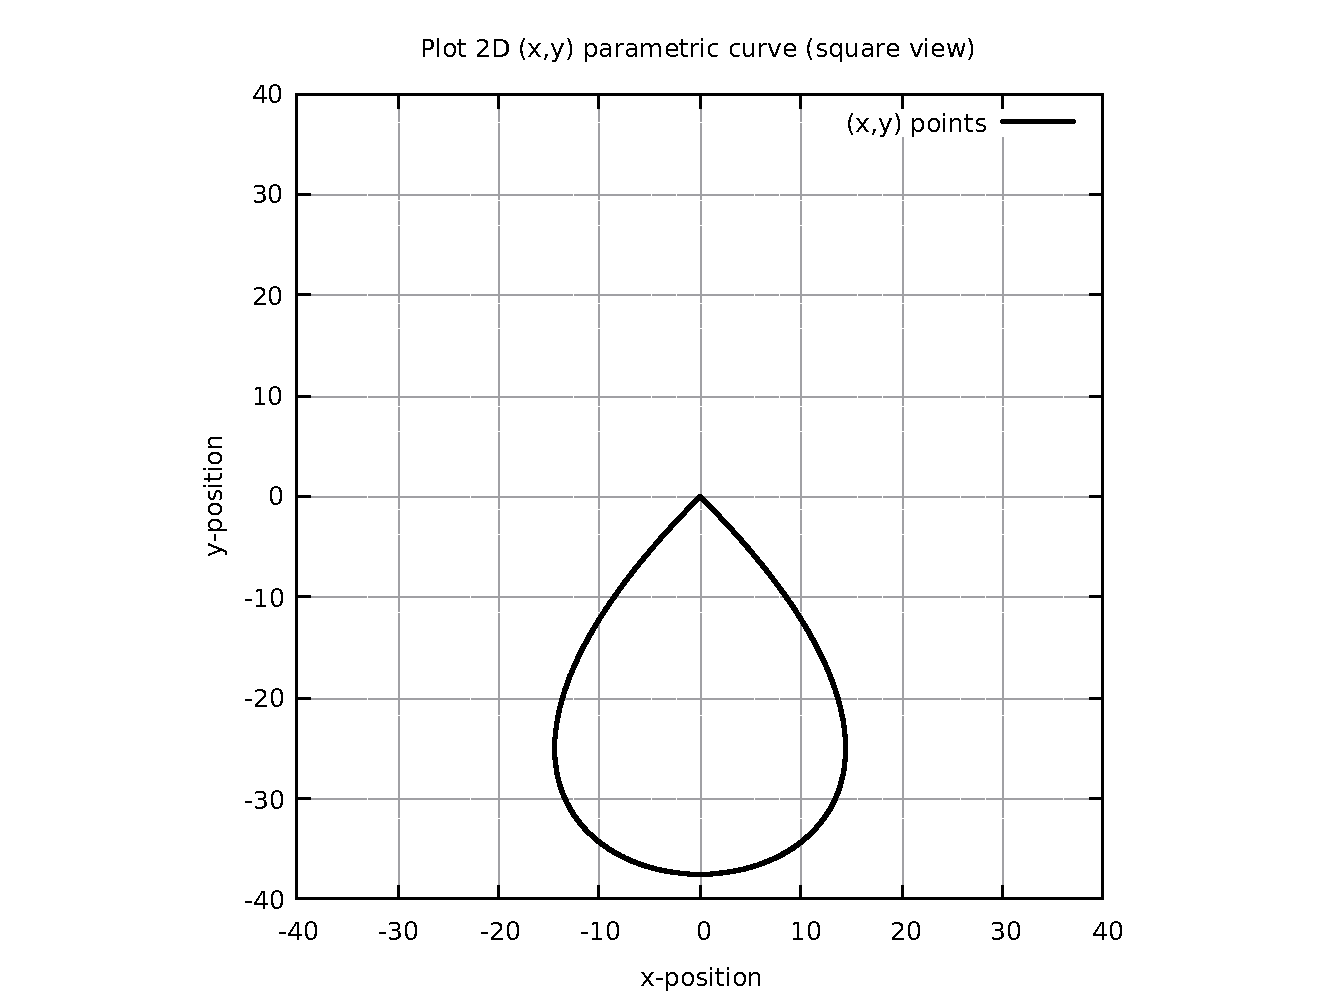
\includegraphics[width=0.90\textwidth]{Chap4/appendix/app-teardrop/img-Plot-of-Teardrop-Curve.pdf} }
\end{figure}	


\begin{figure}
	\caption  {Teardrop Direction of Travel 3D}
	\label{img-chap4-Teardrop Direction of Travel 3D.pdf}
	\centering
	\framebox{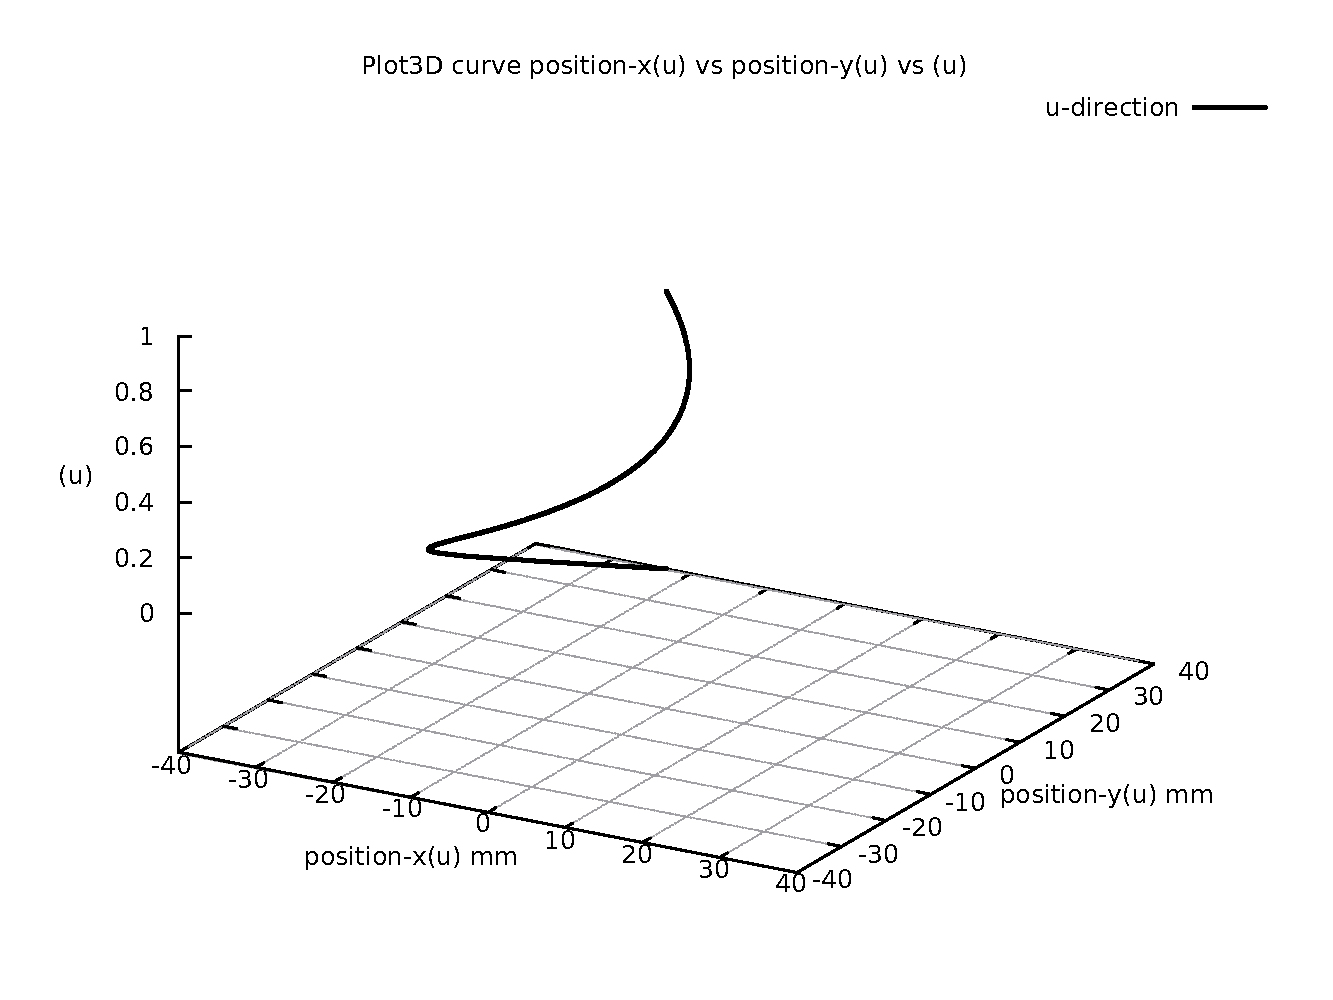
\includegraphics[width=0.90\textwidth]{Chap4/appendix/app-teardrop/img-Teardrop-Direction-of-Travel-3D.pdf} }
\end{figure}

%% ==================================================
\clearpage
\pagebreak

\begin{figure}
	\caption  {Teardrop Perspective View 3D in LinuxCNC-Axis}
	\label{img-chap4-Teardrop-Perspective-View-3D-from-LinuxCNC-Axis.pdf}
	\centering
	\framebox{\includegraphics[width=1.00\textwidth]{Chap4/appendix/app-teardrop/img-Teardrop-Perspective-View-3D-from-Axis.pdf} }
\end{figure}

\subsection{Teardrop Perspective View 3D in LinuxCNC-Axis} 
%%[\ref{img-chap4-Teardrop-Perspective-View-3D-from-LinuxCNC-Axis.pdf}]}
\label{ssec-chap4-Teardrop Perspective View 3D in LinuxCNC-Axis }

The perspective view of the Teardrop curve in Figure [\ref{img-chap4-Teardrop-Perspective-View-3D-from-LinuxCNC-Axis.pdf}] above is a real live validation and verification of the curve running on the LinuxCNC-Axis machine. The software interface panel displays the current position of the cutting tool (cone) as the algorithm drives the tool along the full curve path. \\

In addition, the interface panel also displays the current (x,y) position and velocity (feedrate) of the tool. More will be mentioned on this subject in the section under LinuxCNC-Axis Simulation Run Validation [\ref{ssec-chap4-LinuxCNC-Axis Simulation Run Validation (SRV)}] further in this chapter.


%% ==================================================
\clearpage
\pagebreak

\subsection{Teardrop Radius of Curvature} 
%%[\ref{img-chap4-Teardrop Radius of Curvature.pdf}] } 
\label{ssec-chap4-Teardrop Radius of Curvature} 

The Radius of Curvature rho, for the Teardrop curve is shown in Figure  [\ref  {img-chap4-Teardrop Radius of Curvature.pdf}] on the next page. The correctness of the Radius of Curvature rho(u), is such that it must follow the corresponding curve it represents. \\

For the Teardrop, the value of rho(u) starts high at the beginning because it is near a straight line, and then slowly curve inward thus rho(u) becomes lower, and at the end rho(u) rises high again approaching a near straight line as it reaches its end point.\\

Note that the term "near straight line" have been used because a "true straight line" represents the Radius of Curvature as being infinite, and that there is "no curving" effect at all. On the other hand, a zero value for the Radius of Curvature rho(u), represents a single point, and the curving effect is meaningless. For a typical value of rho(u) like 20, it means the arc segment at that u point is curving like a perfect circle of radius 20. \\ 

Note that the Radius of Curvature rho(u) over the entire parameter range is symmetrical because the Teardrop curve for the parameter (u) movement is symmetrical. If the parameter (u) movement is not symmetrical, for example, the (x,y) point for the start (u = 0.00) is not at the right position, then the Radius of Curvature rho(u) over the entire parameter range is still correct but just not symmetrical. This will be the case for some of the rest of the curves in this work.\\

The Radius of Curvature rho(u), in general, is a good initial visualization tool to validate and indicate correctness of shapes and features of any curve. In this work, the Butterfly has the most complicated Radius of Curvature rho(u) profile. It is shown on the next page in Figure [\ref{img-chap4-Butterfly Radius of Curvature.pdf}]. Further discussion on the Butterfly curve will be made in section under Notable Results Rest of Curves [\ref{Notable Results Rest of Curves}].

%% ==================================================
\clearpage
\pagebreak
	
%% MOVED FORWARD	
%%\begin{figure}
%%	\caption  {Teardrop Perspective View 3D in LinuxCNC-Axis}
%%	\label{img-chap4-Teardrop-Perspective-View-3D-from-LinuxCNC-Axis.pdf}
%%	\centering
%%	\framebox{\includegraphics[width=1.00\textwidth]{Chap4/appendix/app-teardrop/img-Teardrop-Perspective-View-3D-from-Axis.pdf} }
%%\end{figure}

\begin{figure}
	\caption  {Teardrop Radius of Curvature}
	\label{img-chap4-Teardrop Radius of Curvature.pdf}
	\centering
\framebox{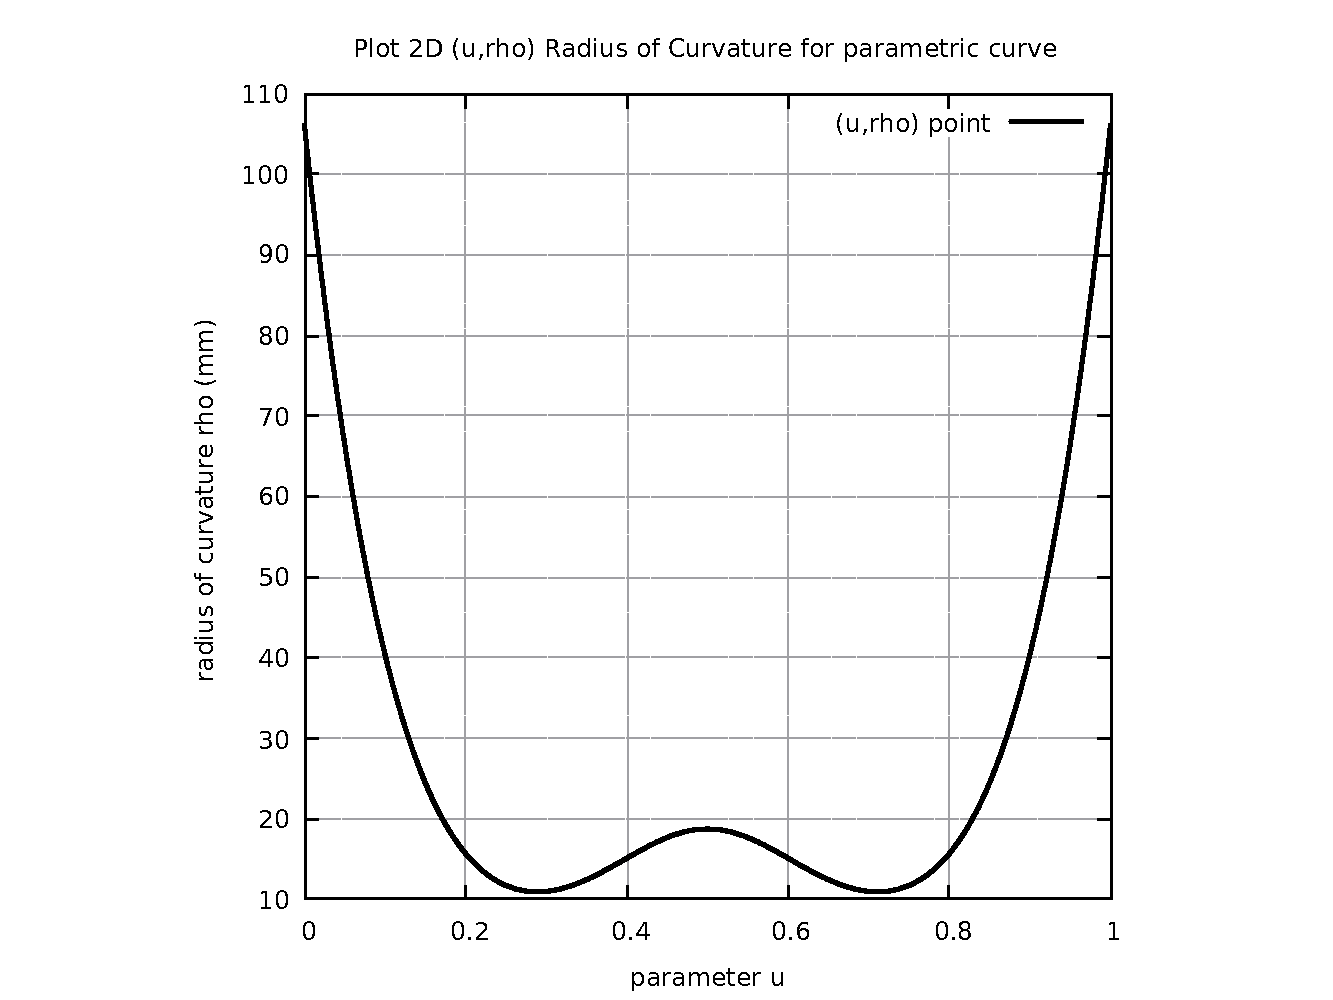
\includegraphics[width=0.90\textwidth]{Chap4/appendix/app-teardrop/img-Teardrop-Radius-of-Curvature.pdf} }
\end{figure}	


\begin{figure}
	\caption  {Butterfly Radius of Curvature}
	\label{img-chap4-Butterfly Radius of Curvature.pdf}
	\centering
\framebox{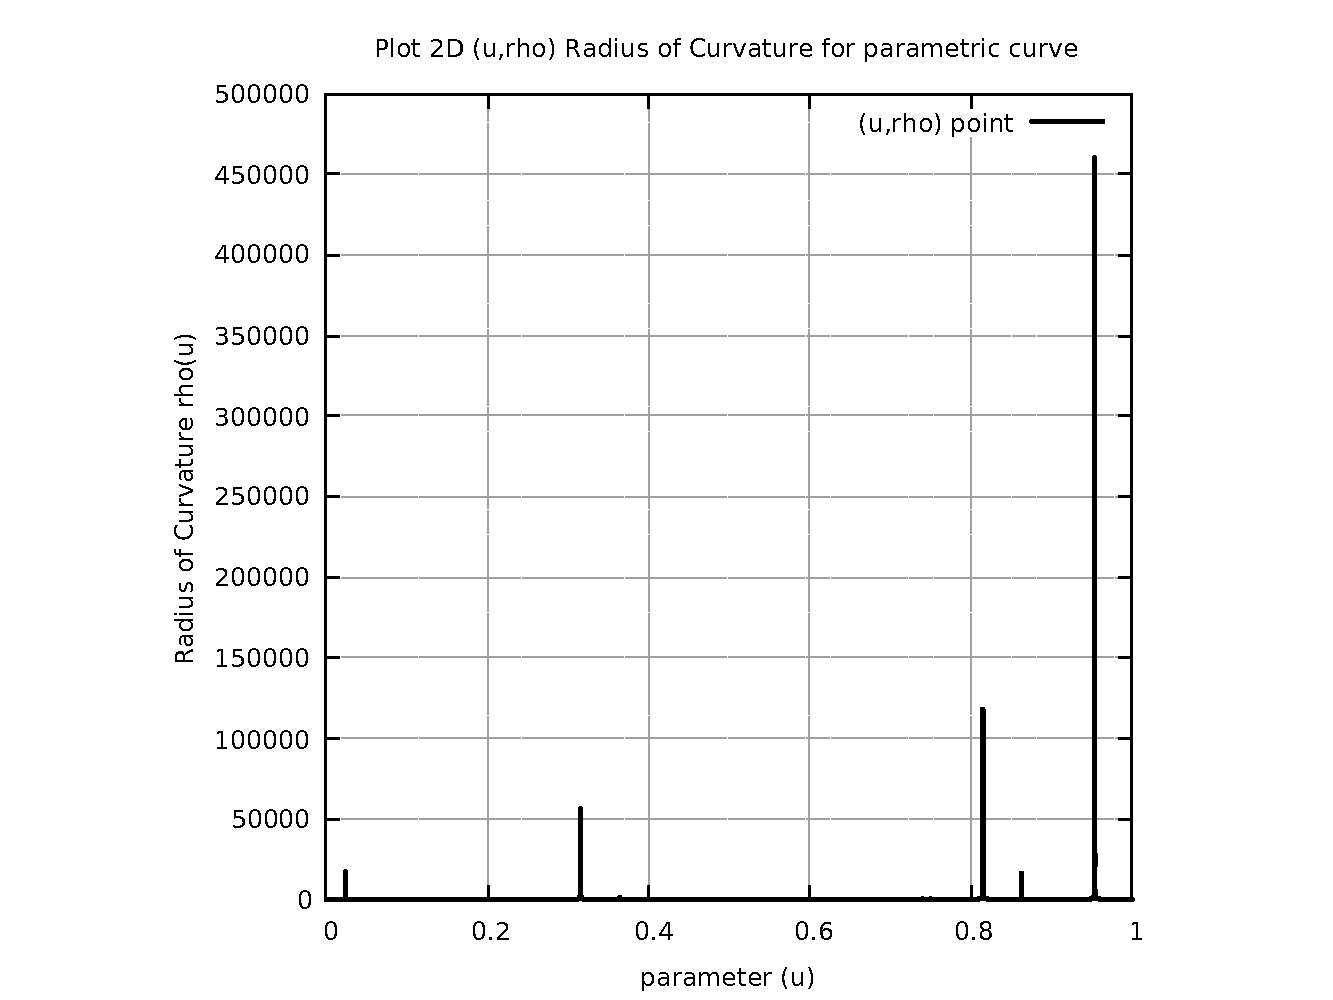
\includegraphics[width=0.90\textwidth]{Chap4/Curves/Butterfly/Butterfly-Radius-of-Curvature.pdf} }
\end{figure}	

%% ==================================================
\clearpage
\pagebreak

\subsection{Teardrop 1st and 2nd Order Taylor's Approximation} 
%% [\ref  {img-chap4-Teardrop 1st and 2nd Order Taylor's Approximation.pdf}]}
\label{ssec-chap4-Teardrop 1st and 2nd Taylor's Approximation}

The results of algorithm execution on the Teardrop curve for the next interpolated point u-next(u) is shown in Figure [\ref  {img-chap4-Teardrop 1st and 2nd Order Taylor's Approximation.pdf}] on the next page. The results comprise the first-order and second-order terms of Taylor's expansion of the curve function C(u) = C(x(u), y(u)), the parametric curve in 2-dimensions. \\

Note that two y-axes were used in this figure, one on the left in magenta and the other on the right in green. The first-order term is the magenta curve, while the second-order term is colored green. Also note that the y-scale on the left was shifted a little bit against the scale on the right. This is to facilitate the separation of the two colored curves. Otherwise, they overlap each other and the difference in values between them is not visible, that is, on the same scale. The next plot handles the difference between the two terms.


\subsection{Teardrop (1st minus 2nd) Order Taylor's Approximation} 
%% [\ref  {img-chap4-Teardrop (1st minus 2nd) Order Taylor's Approximation.pdf}]}
\label{ssec-chap4-Teardrop (1st minus 2nd) Order Taylor's Approximation}

The plot for the difference in value between the first-order and second-order terms in Taylor's approximation is provided in Figure [\ref{img-chap4-Teardrop (1st minus 2nd) Order Taylor's Approximation.pdf}] on the next page. Take note that in Taylor's series expansion, the largest term is the first-order term, the second-order term is smaller, and the third-order term is even smaller, so it continues to an infinite number of smaller terms, theoretically. \\

In addition, the sign of the successive terms in Taylor's series expansion alternates between positive (+) and negative(-), with the starting first-order term being positive (+). That is the reason the plot of the difference is calculated as (first-order - second-order) terms, thus giving a positive value. It is the same reason in separating (shifting) the two curves in the previous figure making the second order term (green) lower than the first-order term (magenta). The difference in value between the two terms exist, but is too small to be visible on the same scale in the previous figure. Therefore, the current figure displays only the difference on a single and expanded y-axis scale.  



%% ==================================================
\clearpage
\pagebreak

\begin{figure}
\caption  {Teardrop 1st and 2nd Order Taylor's Approximation}
\label{img-chap4-Teardrop 1st and 2nd Order Taylor's Approximation.pdf}
\centering
\framebox{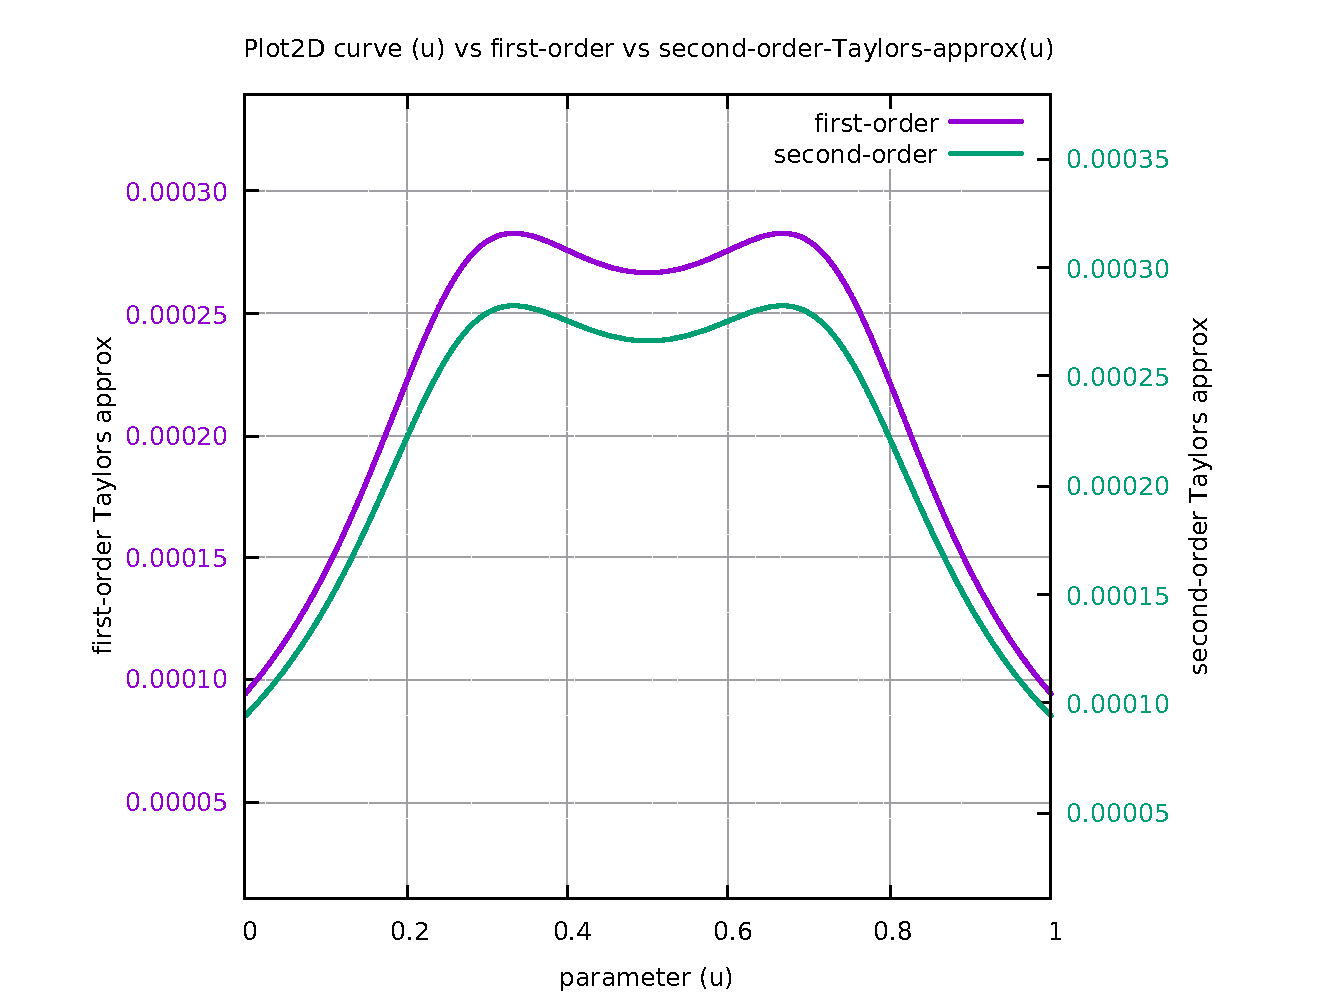
\includegraphics[width=0.90\textwidth]{Chap4/appendix/app-teardrop/img-Teardrop-First-and-Second-Order-Taylors-Approx.pdf} }
\end{figure}	

\begin{figure}
\caption  {Teardrop (1st minus 2nd) Order Taylor's Approximation}
\label{img-chap4-Teardrop (1st minus 2nd) Order Taylor's Approximation.pdf}
\centering
\framebox{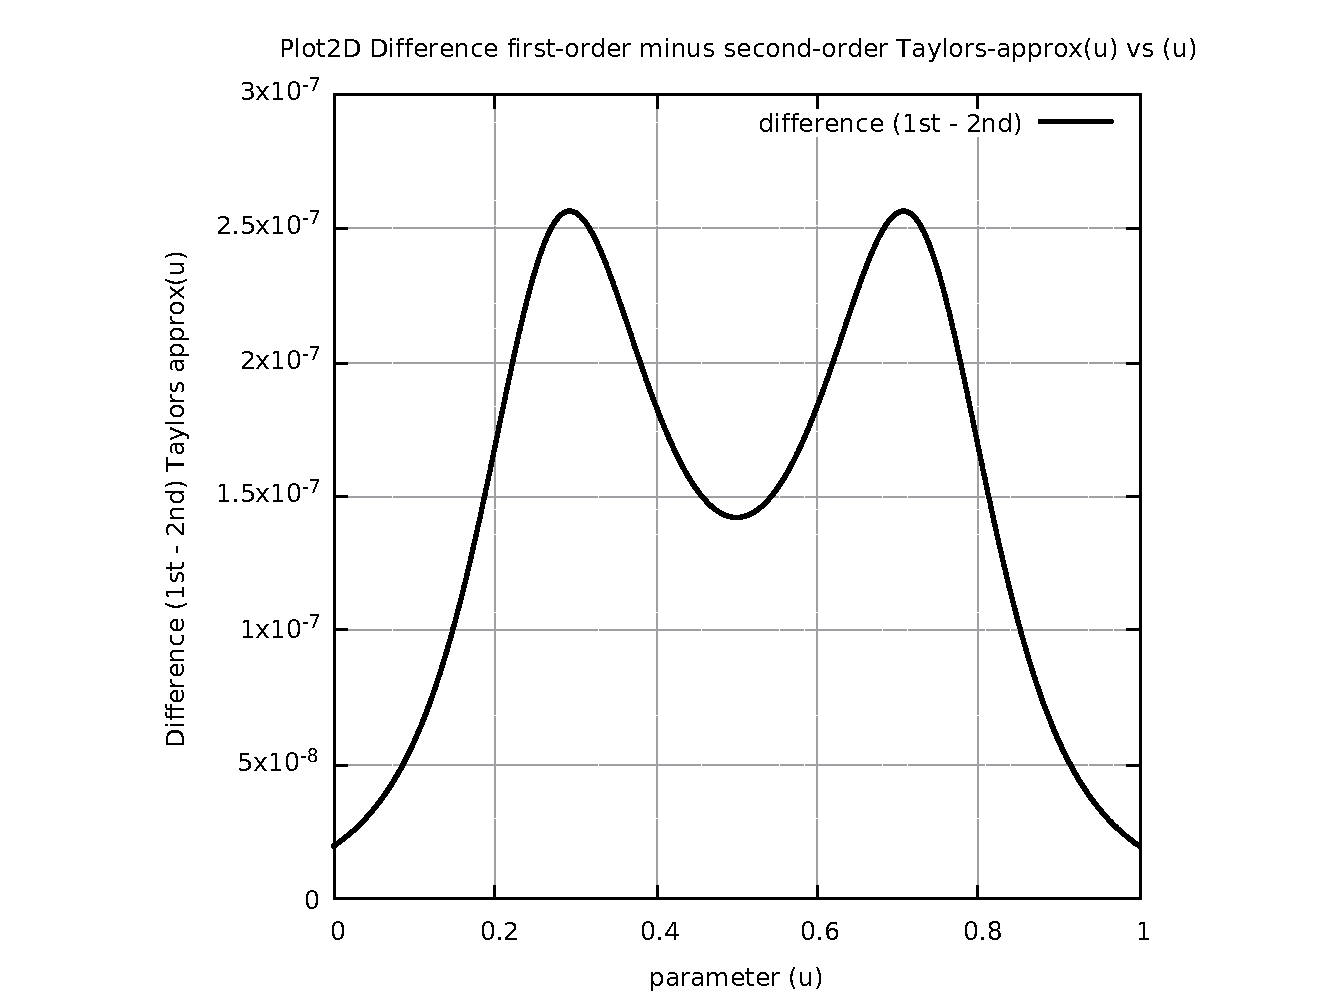
\includegraphics[width=0.90\textwidth]{Chap4/appendix/app-teardrop/img-Teardrop-Difference-First-Second-Order-Taylors-Approximation.pdf} }
\end{figure}	


%% ==================================================
\clearpage
\pagebreak

\subsection{Teardrop Chord-Error Absolute Constraint} 
%% [\ref  {img-chap4-Teardrop Chord-Error Absolute Constraint.pdf}] } 
\label{ssec-chap4-Teardrop Chord-Error Absolute Constraint}

The results for the Teardrop chord-error absolute constraint is provided in Figure [\ref{img-chap4-Teardrop Chord-Error Absolute Constraint.pdf}] on the next page. The two colors (magenta and green) are actually the same data, that is chord-error, but are are plotted on two different scales, the magenta curve using the scale on the left y-axis, while the green curve using the right y-axis. \\

Note that it is the same value data set but plotted on two different scales. The situation is different from the case of the first-order and second-order terms in Taylor's expansion, in which the later comprises two different calculated data sets. This means that if only the magenta curve is displayed for the chord error, a straight horizontal line will be seen in the middle section. \\

The idea for a second expanded scale for the green curve (same chord-error data set), is to visualize the fluctuations or jitters calculated by the algorithm. This graphical plot conclusively shows that the chord-error(u) at every u-point in the full range of $(0.00 \le u \le 1.00)$ lies below the chord-error tolerance, which was set at 1E-6 mm.\\ 

This absolute constraint on chord-error is one of the main objectives of the algorithm in this thesis.


\subsection{Teardrop Four(4) Feedrate Limit Components Profile}
%% [\ref  {img-chap4-Teardrop Four Feedrate Limit Components Profile.pdf}] }
\label{ssec-chap4-Teardrop Four Feedrate Limit Components Profile}

The results for the Teardrop four(4) feedrate limit components is provided in Figure [\ref{img-chap4-Teardrop Four Feedrate Limit Components Profile.pdf}] on the next page. The value of the feedrate limit at any point u, Feedrate\_Limit(u), is the minimum value among the four components, evaluated at the same point u. \\

The figure shows the yellow curve is the most dominant (lowest value) among the 4 limit components throughout the middle range, outside of the rising S-curve and falling S-curve sections. The yellow curve is Limit-4, the Acceleration Confinement limit.\\

This plot is based on the Teardrop curve running at FC20 and lamda = 0.18 (restrictive acceleration confinement). If the value of lamda is increased, for example, to lamda = 0.25 (relaxed acceleration confinement), then the yellow curve will increase, thus, criss-crossing with the blue curve (Limit-3, Chord-error accuracy). This resulted in the minimum value changing between these two curves. This is how the value of the Feedrate\_Limit(u) is calculated by the algorithm.\\  

As explained in the earlier section under Results for finding acceptable lamda at reference [\ref{ssec-Results for finding acceptable lamda}], the value of Lamda = 0.25 for the Teardrop curve running at FC20 will definitely cause acceleration jitters, thus making the running feedrate jerky in the affected regions. This result violates the requirement for absolute smoothness in feedrate, which is one of the main objectives of the interpolation algorithm in this thesis.


%% PLOTS
%% ==================================================
\clearpage
\pagebreak

\begin{figure}
	\caption  {Teardrop Chord-Error Absolute Constraint}
	\label{img-chap4-Teardrop Chord-Error Absolute Constraint.pdf}
	%% \centering
	\framebox{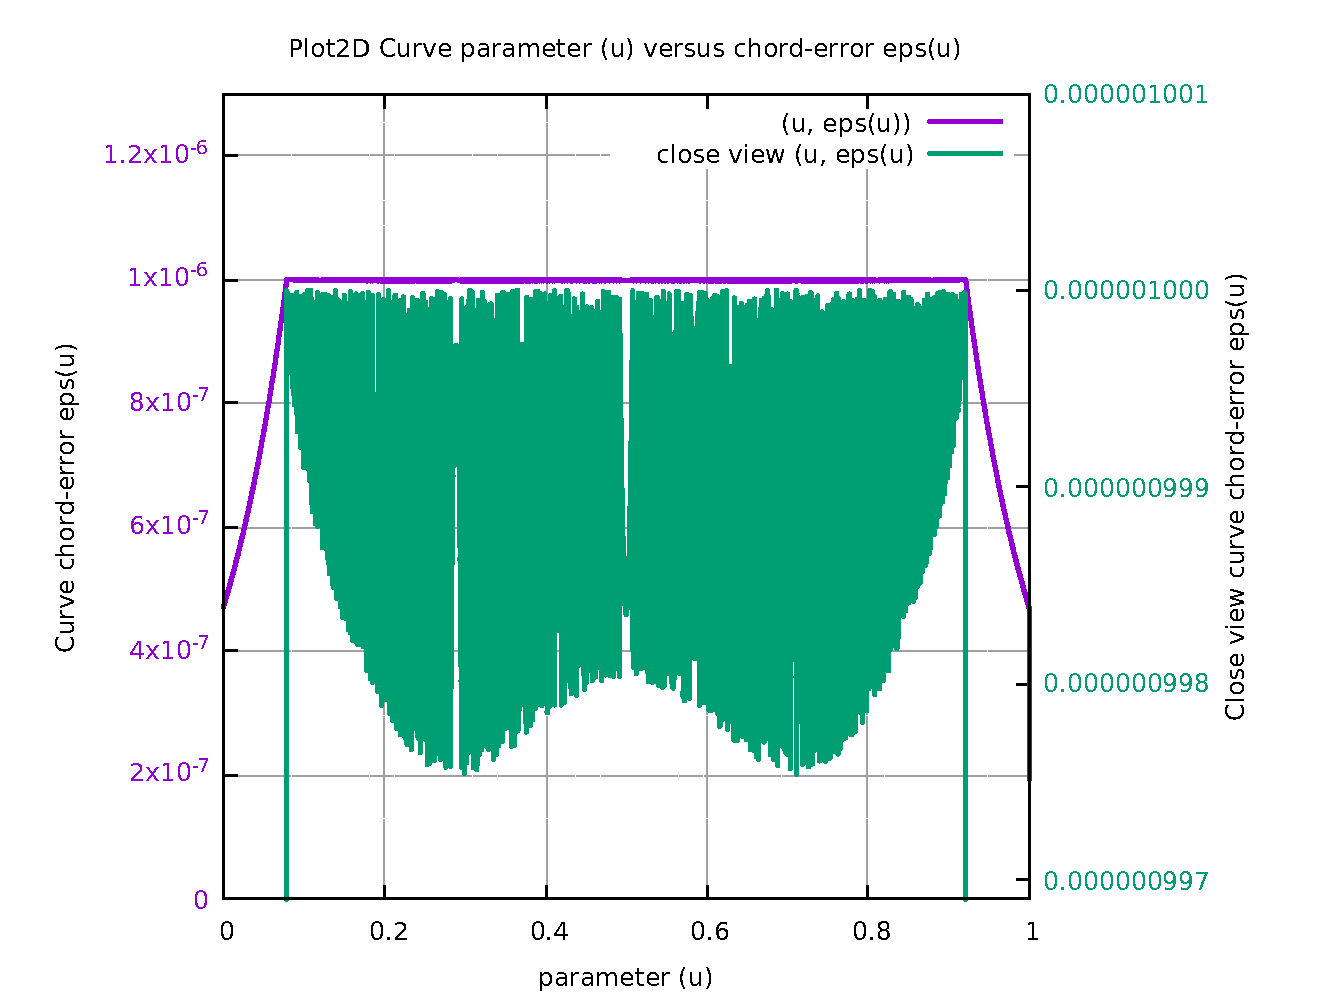
\includegraphics[width=0.90\textwidth]{Chap4/appendix/app-teardrop/img-Teardrop-Chord-Error-Absolute-Constraint.pdf} }
\end{figure}	

\begin{figure}
	\caption  {Teardrop Four Feedrate Limit Components Profile}
	\label{img-chap4-Teardrop Four Feedrate Limit Components Profile.pdf}
	%% \centering 
	\framebox{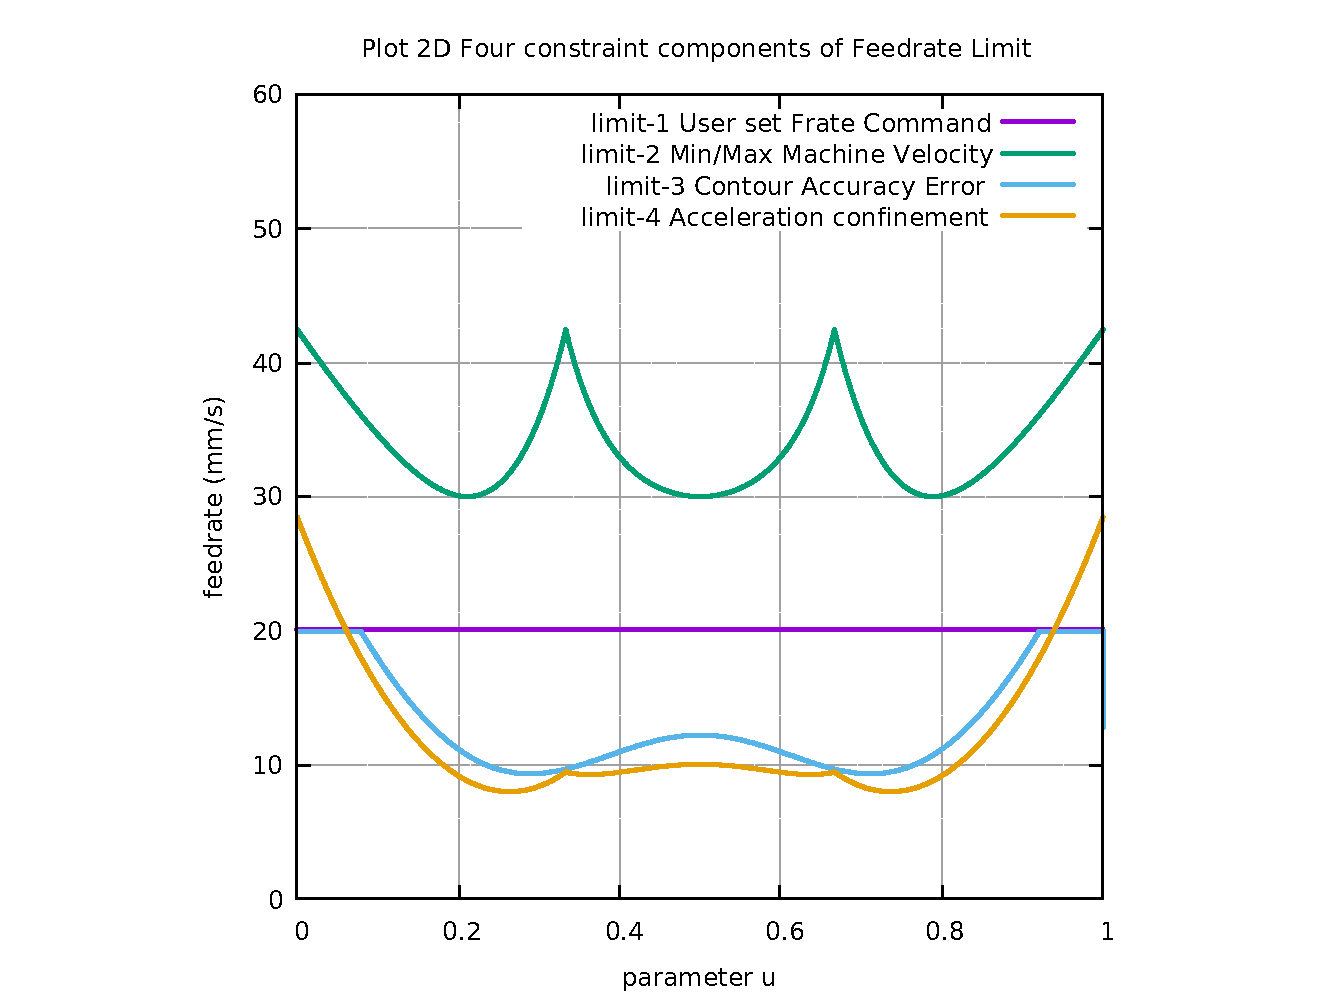
\includegraphics[width=0.90\textwidth]{Chap4/appendix/app-teardrop/img-Teardrop-Four-Constraint-Components-of-Feedrate-Limit.pdf} }
\end{figure}	

%% ==================================================
\clearpage
\pagebreak

\subsection{Teardrop FRate Command, FRate Limit, Current FRate}
%% [\ref  {img-chap4-Teardrop-FeedrateCommand-FeedrateLimit-CurrentFeedrate.pdf}] }
\label{ssec-chap4-Teardrop-FeedrateCommand-FeedrateLimit-CurrentFeedrate}

The Teardrop curve execution giving results for the Feedrate Limit and the  Current Feedrate is shown in Figure [\ref{img-chap4-Teardrop-FeedrateCommand-FeedrateLimit-CurrentFeedrate.pdf}] on the next page. The terms current feedrate and running feedrate are used interchangeably in this document.

The Feedrate Command FC is a user specified constant value, and in this case FC = 20 mm/s. The Feedrate Limit is calculated by the interpolation algorithm at every parameter point u based on the minimum of four(4) feedrate component limits. The Current or Running Feedrate is recursively calculated by the algorithm as close to but below the Feedrate Limit.\\

In the figure, only two(2) of the three(3) curves are visible. This is due to the Current or Running Feedrate is seen as overlapping with the Feedrate Limit. In reality their values are close but different, and will be shown in the next figure.


\subsection{Teardrop Current Feedrate Absolute Constraint}
%% [\ref  {img-chap4-Teardrop Current Feedrate Absolute Constraint.pdf}] }
\label{ssec-chap4-Teardrop Current Feedrate Absolute Constraint}

Figure [\ref{img-chap4-Teardrop Current Feedrate Absolute Constraint.pdf}] displays the difference in value between the Feedrate Limit and current or running feedrate for the Teardrop curve.\\

The display shows positive or zero value difference in blue color for the entire range of u values of the Teardrop curve, without exception. This means that the feedrate limit is always higher than the running feedrate, even though the difference is very small. There are no negative differences. Therefore, the running feedrate is constrained to be below the feedrate limit.\\  

This absolute constraint on running feedrate is one of the main objectives of the algorithm in this thesis.

%% PLOTS
%% ==================================================
\clearpage
\pagebreak

\begin{figure}
	\caption  {Teardrop FRate Command, FRate Limit and Current FRate}
	\label{img-chap4-Teardrop-FeedrateCommand-FeedrateLimit-CurrentFeedrate.pdf}
	%% \centering
	\framebox{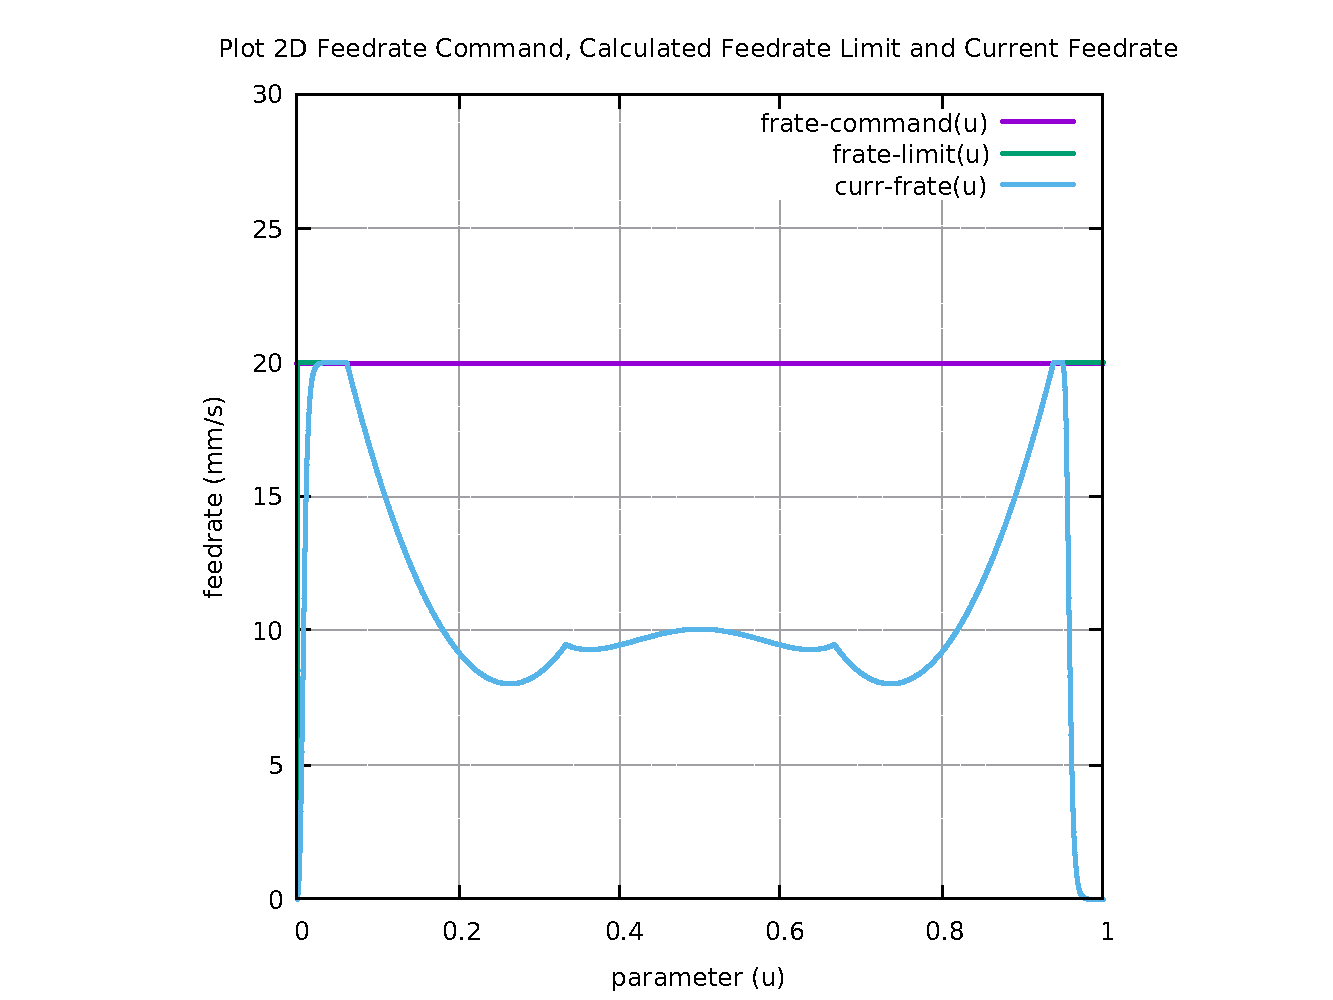
\includegraphics[width=0.90\textwidth]{Chap4/appendix/app-teardrop/img-Teardrop-FeedrateCommand-FeedrateLimit-CurrentFeedrate.pdf} }
\end{figure}	

\begin{figure}
	\caption  {Teardrop Current Feedrate Absolute Constraint}
	\label{img-chap4-Teardrop Current Feedrate Absolute Constraint.pdf}
	%% \centering
	\framebox{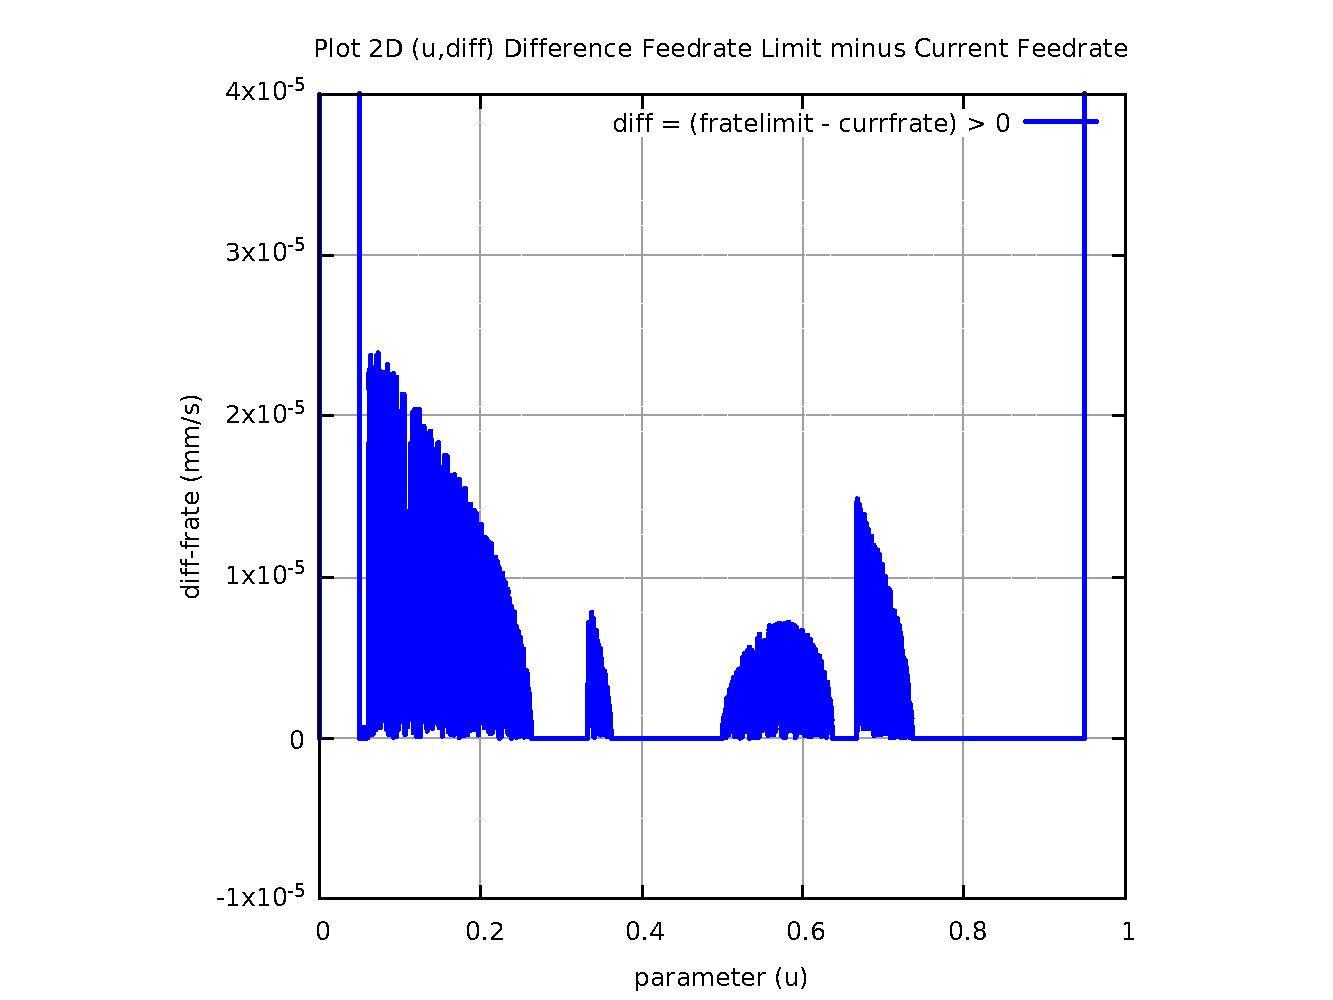
\includegraphics[width=0.90\textwidth]{Chap4/appendix/app-teardrop/img-Teardrop-Difference-Feedrate-Limit-and Current-Feedrate-positive.pdf} }
\end{figure}	

%% ==================================================
\clearpage
\pagebreak

\subsection{Teardrop Histogram distribution of interpolated points}
%% [\ref  {img-chap4-Teardrop Histogram distribution of interpolated points.pdf}]}
\label{ssec-chap4-Teardrop Histogram distribution of interpolated points}

Figure [\ref{fig-chap4-Teardrop Histogram distribution of interpolated points}] shows a histogram for the distribution of interpolated point for the Teardrop curve covering the full range of parameter u, $(u = 0.00 \le u \le 1.00)$, divided into 10 bins of width 0.10 each. \\

The histogram was generated for the common lamda = 0.18 and four(4) Feedrate Commands comprising FC10, FC20, FC30 and FC40. The corresponding data table that was used to generate this histogram is provided in the next section.


\subsection{Teardrop Table distribution of interpolated points}
%% [\ref  {tab-chap4-Teardrop Table distribution of interpolated points.tex}] }
\label{ssec-chap4-Teardrop Table distribution of interpolated points}

Table [\ref{tab-chap4-Teardrop Table distribution of interpolated points}] shows the resulting data for the different Feedrate Command FC, execution runs of the algorithm against the Teardrop curve. \\

Generally, the total number of interpolated points decreases as the Feedrate Command increases. This can be seen in the last row of the data table. This makes sense since for the same total length of the Teardrop curve, an increase in FC means an increase in feedrate, thus increasing the chord-length of travel during the same interpolation period (constant delta time 0.001 s). This increase in chord-length means a decrease in total interpolated points. The side effect is an increase in the total sum-chord-error since each chord-length increases.\\

The concept of Total Interpolated Points (TIP) for a single curve like the Teardrop curve does not give much useful information in itself. But when comparisons are made for Total Interpolated Points (TIP) of all ten(10) parametric curves, the interpretation will provide useful information. This is one of the objectives of this thesis. The subject is handled in a later section under Overall Execution Results at Reference [\ref{sec-OVERALL EXECUTION RESULTS}].  


%% PLOTS OR HISTOGRAM TABLES
%% =============================
%% ==================================================
\clearpage
\pagebreak

\begin{figure}
	\centering
	\caption    {Teardrop Histogram distribution of interpolated points}
	\label  {fig-chap4-Teardrop Histogram distribution of interpolated points}
	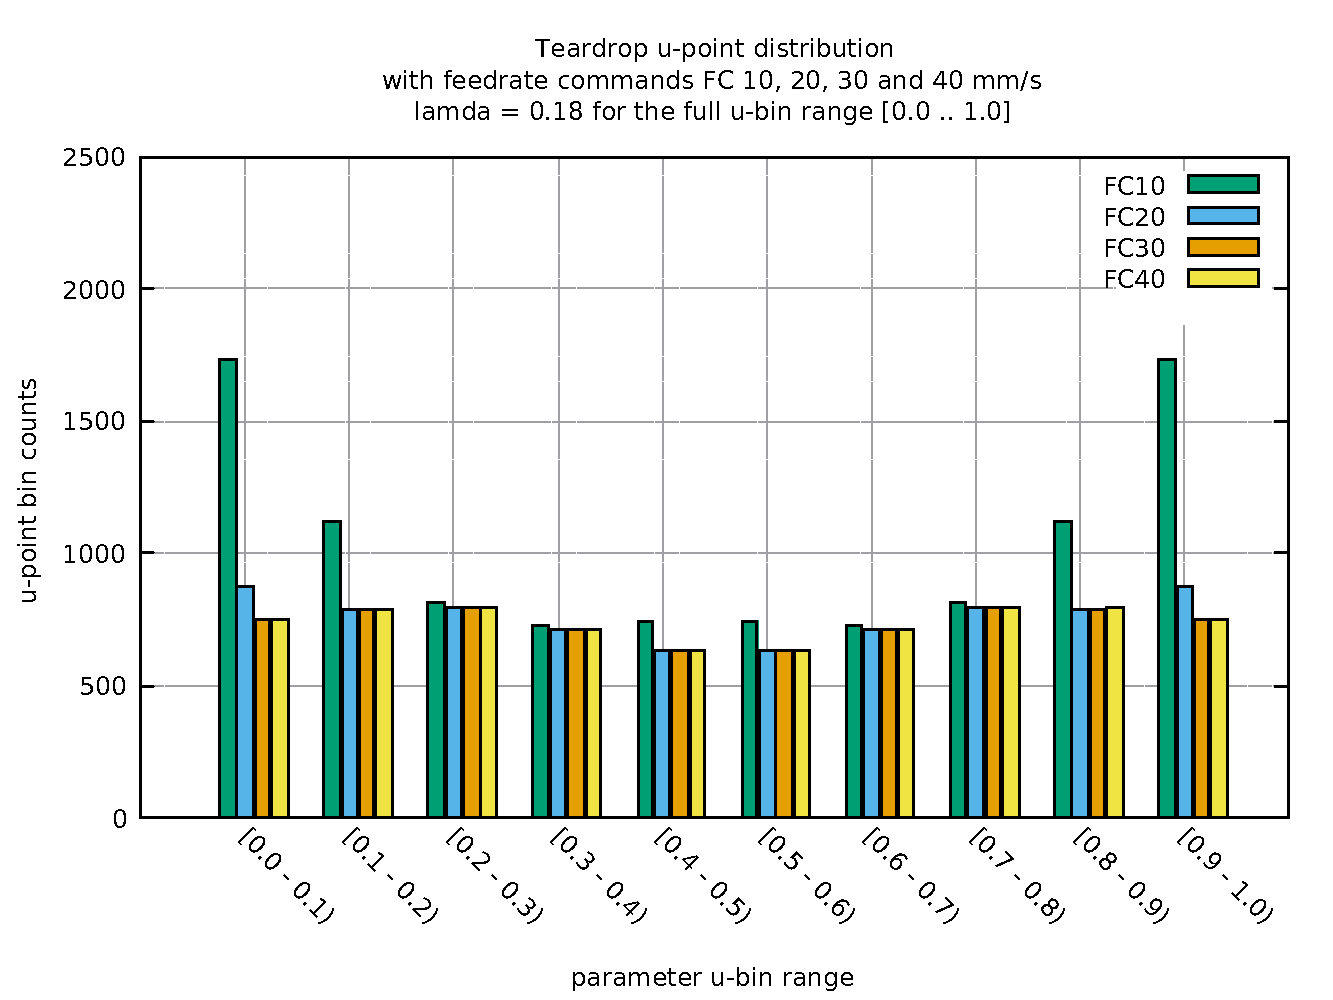
\includegraphics[width=1.00\textwidth]{Chap4/Teardrop/distributions/Teardrop-u-distribution-FCXX-L018-Algo28.pdf} 
	
\end{figure}


\begin{table}[ht]
	%% \begin{center}
	\caption    {Teardrop Table distribution of interpolated points}
	\label  {tab-chap4-Teardrop Table distribution of interpolated points}
	
	%% IMPORTANT TO SCALEBOX BELOW
	\scalebox{0.80}{
		
		%% START COPY AND PASTE BELOW HERE
		%% FROM \begin{tabular} UNTIL \end{tabular)
		%% Note: adjust last p{} to get line width correct
		
		\begin{tabular}{ p{4.5cm} p{1.5cm} p{1.5cm} p{1.5cm} p{7.50cm} }
			\hline
			&		    &		 &		  &	    \\
			BINS	    &	FC10 &  FC20  &  FC30  &  FC40  \\
			&		    &	     &		  &	     \\
			0.0 – 0.1	&	1734 &	875	  &	748	   &	748	\\
			0.1 – 0.2	&	1120 &	791	  &	791	   &	791	\\
			0.2 – 0.3	&	809	 &	794	  &	794	   &	794	\\
			0.3 – 0.4	&	726	 &	710	  &	711	   &	711	\\
			0.4 – 0.5	&	741	 &	629	  &	629	   &	629	\\
			0.5 – 0.6	&	742	 &	629	  &	628	   &	629	\\
			0.6 – 0.7	&	726	 &	710	  &	711	   &	711	\\
			0.7 – 0.8	&	809	 &	794	  &	794	   &	793	\\
			0.8 – 0.9   &	1120 &	791	  &	791	   &	792	\\
			0.9 – 1.0	&	1734 &	876	  &	750	   &	749	\\
			&		    &		 &		  &		\\
			Total counts&  10261 &	7599  &	7347   &   7347	\\
			&		    &		 &		  &		
			
		\end{tabular}
		
		%% END COPY AND PASTE ABOVE HERE
		
	}   %% IMPORTANT FOR SCALEBOX CLOSING
	
	\hrule
\end{table}
%% \end{landscape}

%% ==================================================
\clearpage
\pagebreak
\subsection{Teardrop Rising Current Feedrate Profile}
%% [\ref  {img-chap4-Teardrop Rising Current Feedrate Profile.pdf}]}
\label{ssec-chap4-Teardrop Rising Current Feedrate Profile}

The profiles for the rising feedrate curves are shown in Figure [\ref{img-chap4-Teardrop Rising Current Feedrate Profile.pdf}] on the next page. The parameter range for the S-curve rise is set at $(0.00 \le u \le 0.05)$ or 5 percent of the total interpolated points. The lamda value chosen is 0.18 and the Feedrate Command is 20.0 mm/s.\\

It should be noted that throughout both the rising and falling regions, the S-curve equation is only used to set the Feedrate\_Limit(u) and not the Running\_Feedrate(u). The algorithm still calculates the running feedrate and the chord-error, during which, both of their constraints are maintained. This ensures that there are no exceptions in the algorithm that both or either one of the constraints are violated. Both must not be violated, absolutely. 


\subsection{Teardrop Falling Current Feedrate Profile}
%% [\ref  {img-chap4-Teardrop Falling Current Feedrate Profile.pdf}]}
\label{ssec-chap4-Teardrop Falling Current Feedrate Profile}

The profiles for the falling feedrate curves are shown in Figure [\ref{img-chap4-Teardrop Falling Current Feedrate Profile.pdf}] on the next page. The parameter range for the S-curve fall is set at $(0.95 \le u \le 1.00)$ or also 5 percent of the total interpolated points. The lamda value chosen is 0.18 and the Feedrate Command is 20.0 mm/s.\\



%% PLOTS
%% =============
\clearpage
\pagebreak

\begin{figure}
	\caption  {Teardrop Rising Current Feedrate Profile}
	\label{img-chap4-Teardrop Rising Current Feedrate Profile.pdf}
	%% \centering
	\framebox{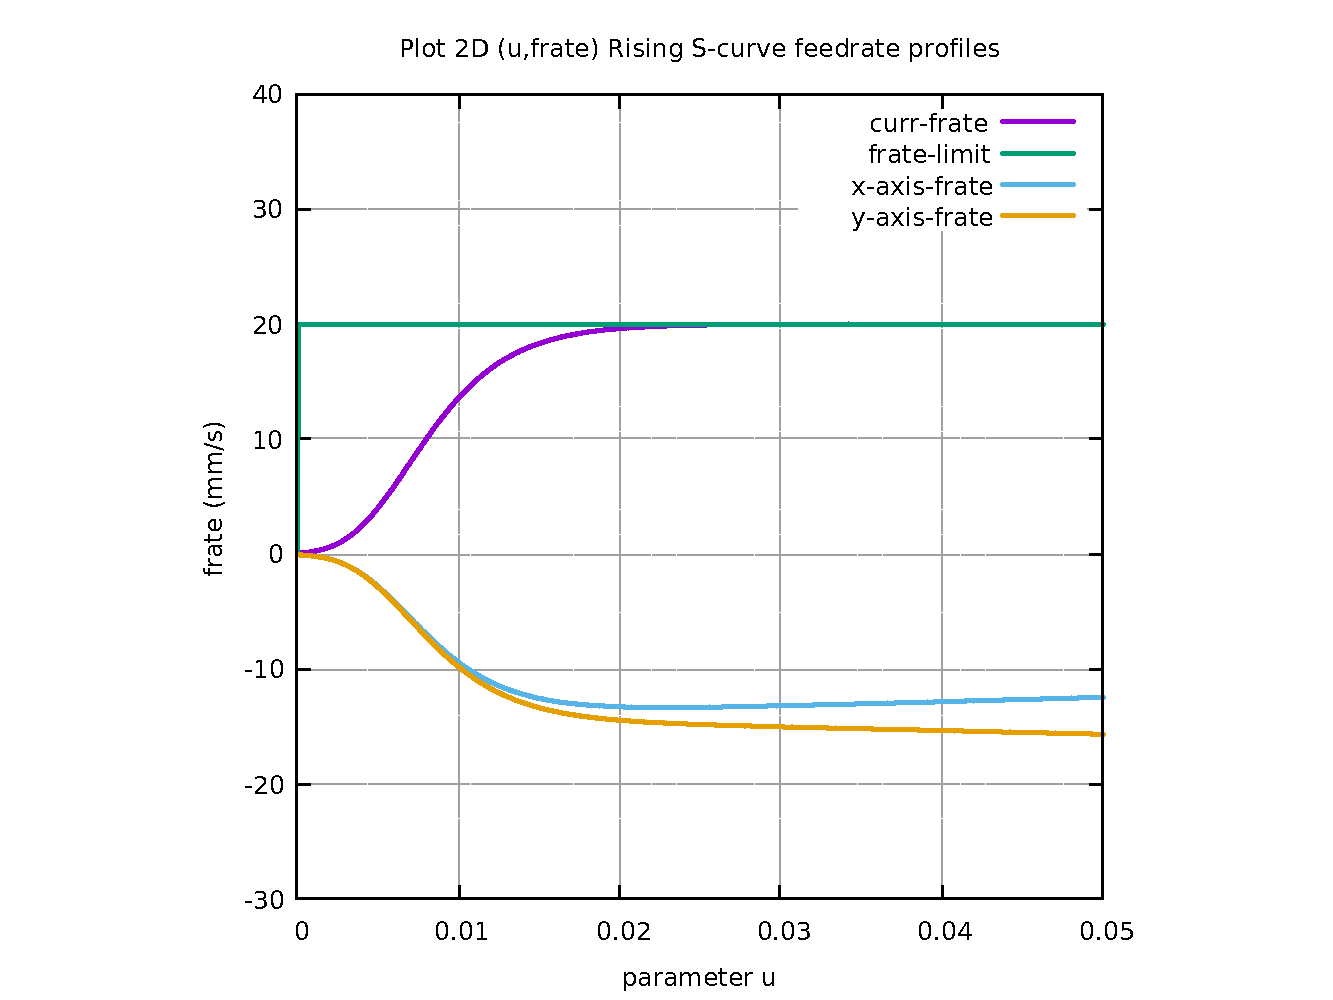
\includegraphics[width=0.90\textwidth]{Chap4/appendix/app-teardrop/img-Teardrop-Rising-Feedrate-S-Curve-Profiles.pdf} }
\end{figure}	

\begin{figure}
	\caption  {Teardrop Falling Current Feedrate Profile}
	\label{img-chap4-Teardrop Falling Current Feedrate Profile.pdf}
	%% \centering
	\framebox{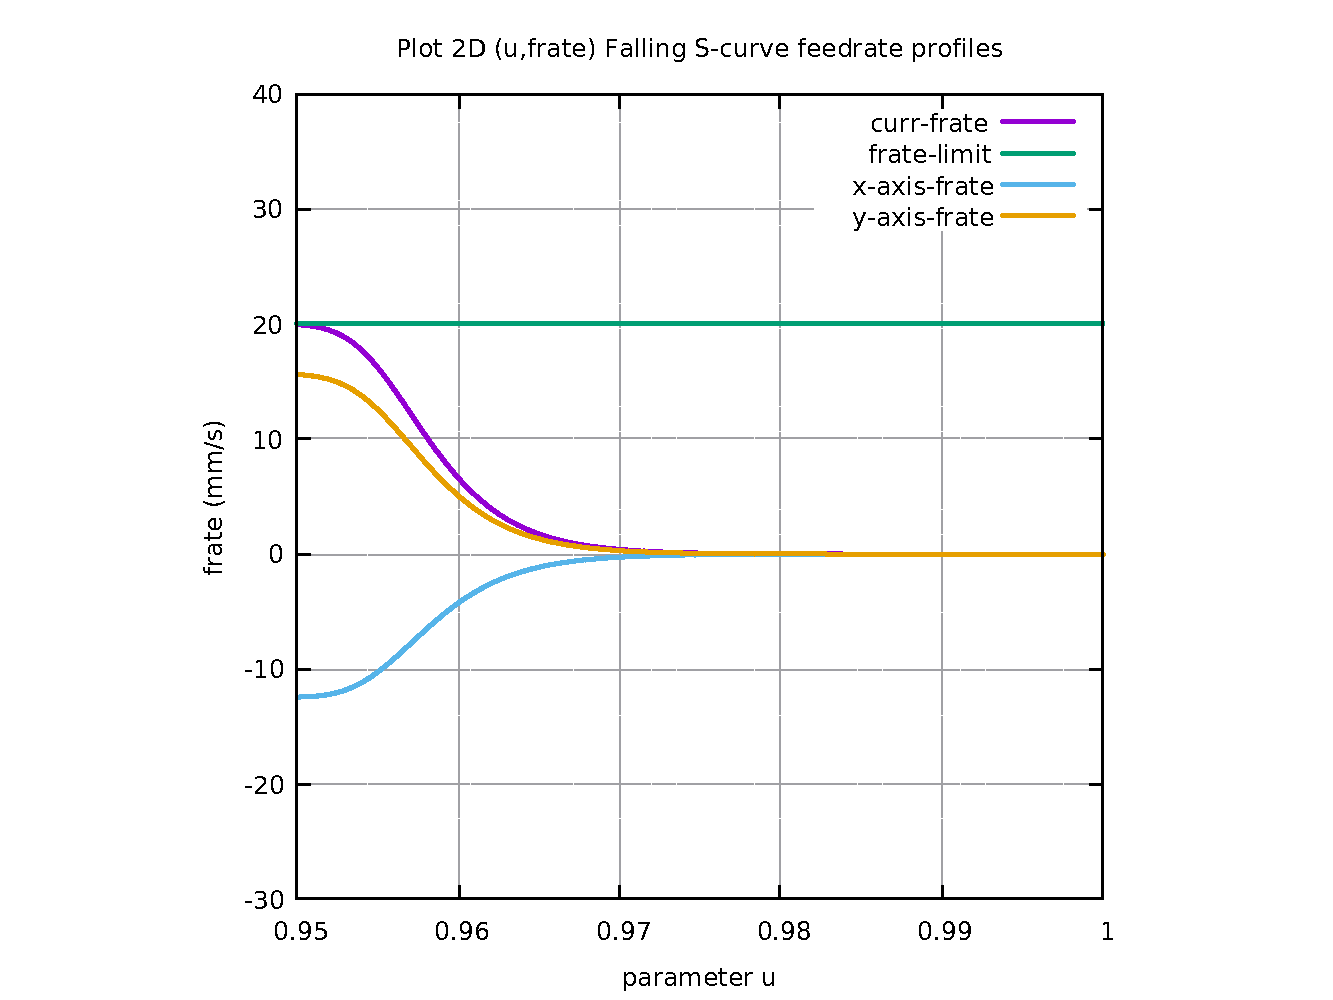
\includegraphics[width=0.90\textwidth]{Chap4/appendix/app-teardrop/img-Teardrop-Falling-Feedrate-S-Curve-Profiles.pdf} }
\end{figure}	

%% ==================================================
\clearpage
\pagebreak

\subsection{Teardrop FC10, FC20, TC30 \& FC40 Running Feedrates}
%% [\ref  {img-chap4-Teardrop-FC10-Running-Feedrate-Profiles.pdf}] }
\label{ssec-chap4-Teardrop-FC10-Running-Feedrate-Profiles}

The next two(2) pages show four(4) execution results for the Teardrop curve at lamda = 0.18 for feedrate commands FC10, FC20, FC30 and FC40, in Figure [\ref{img-chap4-Teardrop-FC10-Running-Feedrate-Profiles.pdf}], 
Figure [\ref{img-chap4-Teardrop-FC20-Running-Feedrate-Profiles.pdf}], 
Figure [\ref{img-chap4-Teardrop-FC30-Running-Feedrate-Profiles.pdf}] and 
Figure [\ref{img-chap4-Teardrop-FC40-Running-Feedrate-Profiles.pdf}], respectively.\\

The next four(4) plots show that all of the running feedrates remain below the respective feedrate command FC. This is a constraint that cannot be violated in all circumstances. \\

These plots cover the feedrate rising region (5 \% points), the main feedrate activity region (90 \% points), and the feedrate falling region (5 \% points). \\

The first plot for FC10, shows that a significant portion of the current (running) feedrate flattens at the 10 mm/s level (FC10). The second plot for FC20 shows a small portion of the current feedrate flattens at the 20 mm/s level (FC20). In the case of both the third and fourth plots (FC30 and FC40) respectively, their current feedrates never reach their set Feedrate Command levels. \\

It is important to remember that the feedrate limit is different from the current or running feedrate. Both feedrates are nearly equal in value, with running feedrate always just a little lower than the feedrate limit. Both feedrates vary with parameter u, unlike the feedrate command (FC), which is a constant. They are not displayed in the plots because they essentially overlap due to a relatively large y-scale display.  \\

The x-axis and y-axis feedrates are self-explanatory. A negative value means moving in the opposite direction. The magnitude of the feedrate (a scalar) remains the same.


%% PLOTS
%% ==================
%% ==================
\clearpage
\pagebreak

\begin{figure}
	\caption  {Teardrop FC10 Running Feedrate Profiles}
	\label{img-chap4-Teardrop-FC10-Running-Feedrate-Profiles.pdf}
	%% \centering
	\framebox{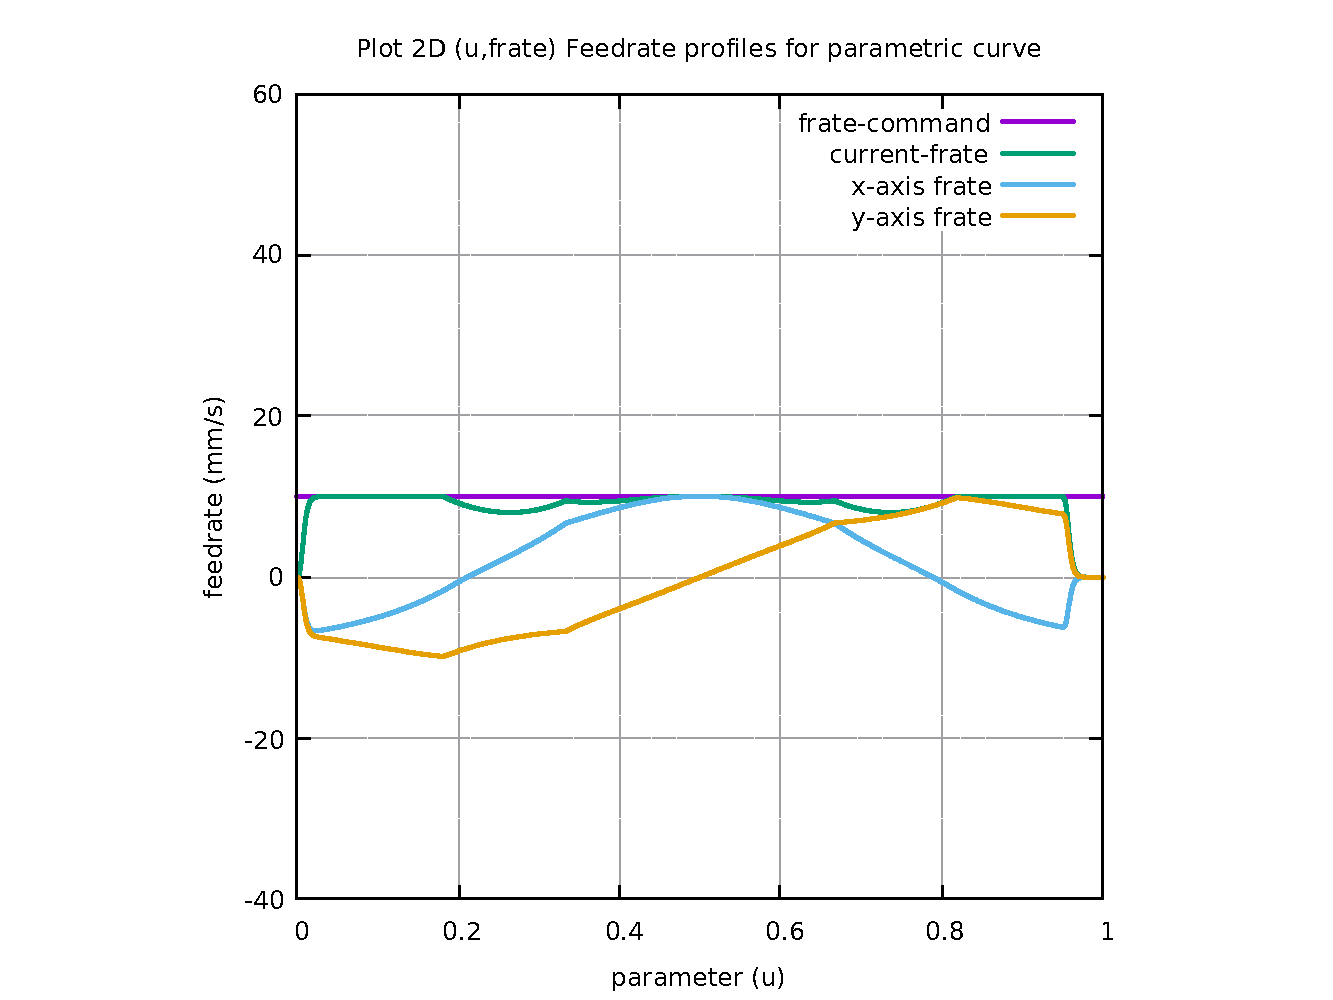
\includegraphics[width=0.90\textwidth]{Chap4/appendix/app-teardrop/img-Teardrop-FC10-Running-Feedrate-Profiles.pdf} }
\end{figure}	

\begin{figure}
	\caption  {Teardrop FC20 Running Feedrate Profiles}
	\label{img-chap4-Teardrop-FC20-Running-Feedrate-Profiles.pdf}
	%% \centering
	\framebox{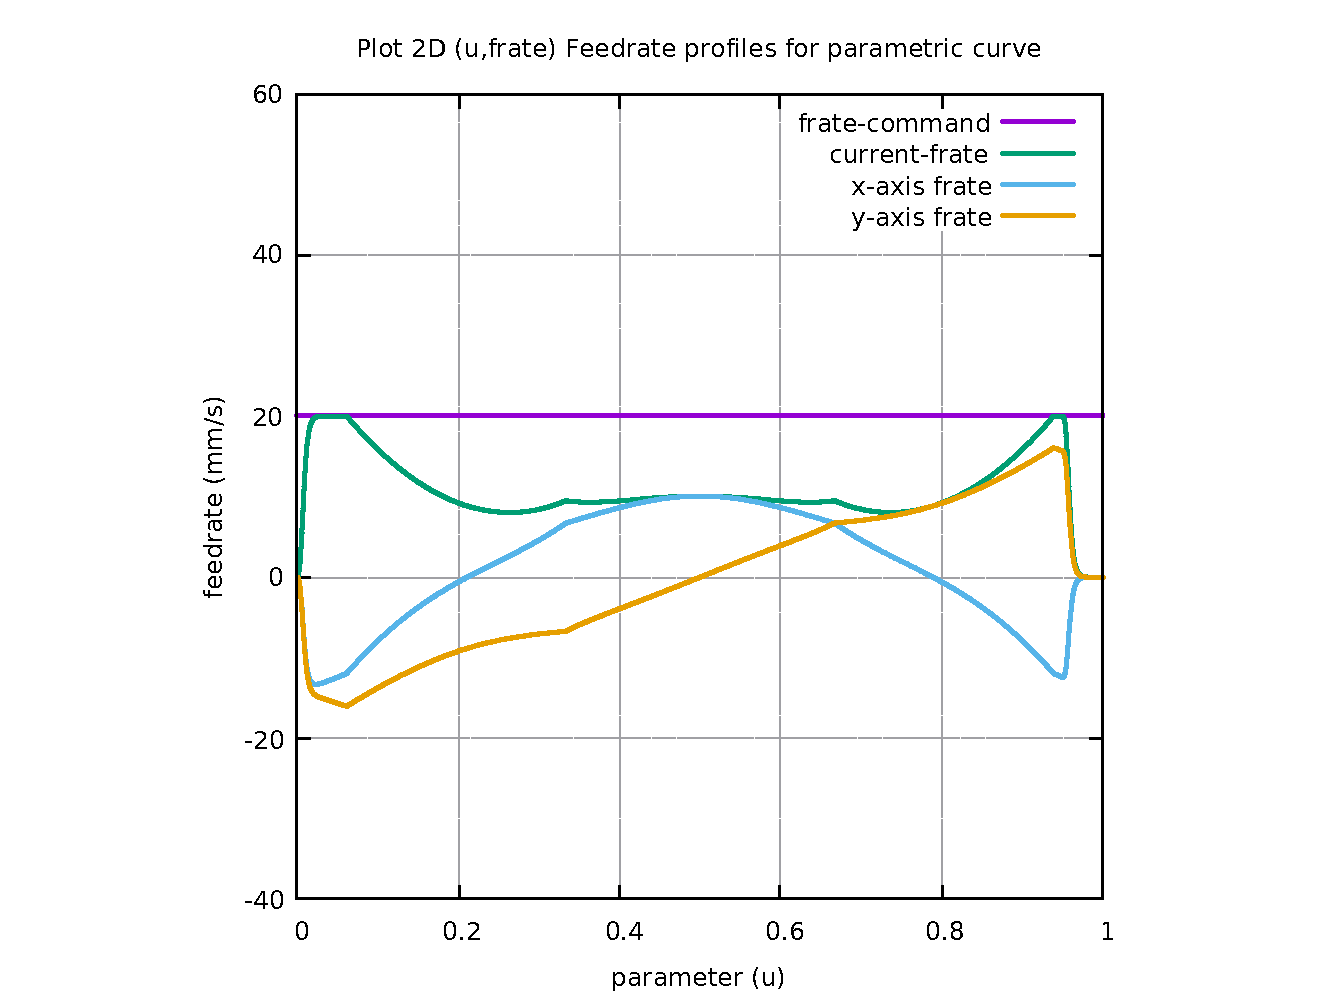
\includegraphics[width=0.90\textwidth]{Chap4/appendix/app-teardrop/img-Teardrop-FC20-Running-Feedrate-Profiles.pdf} }
\end{figure}	

%% ==================================================
\clearpage
\pagebreak

\begin{figure}
	\caption  {Teardrop FC30 Running Feedrate Profiles}
	\label{img-chap4-Teardrop-FC30-Running-Feedrate-Profiles.pdf}
	%% \centering
	\framebox{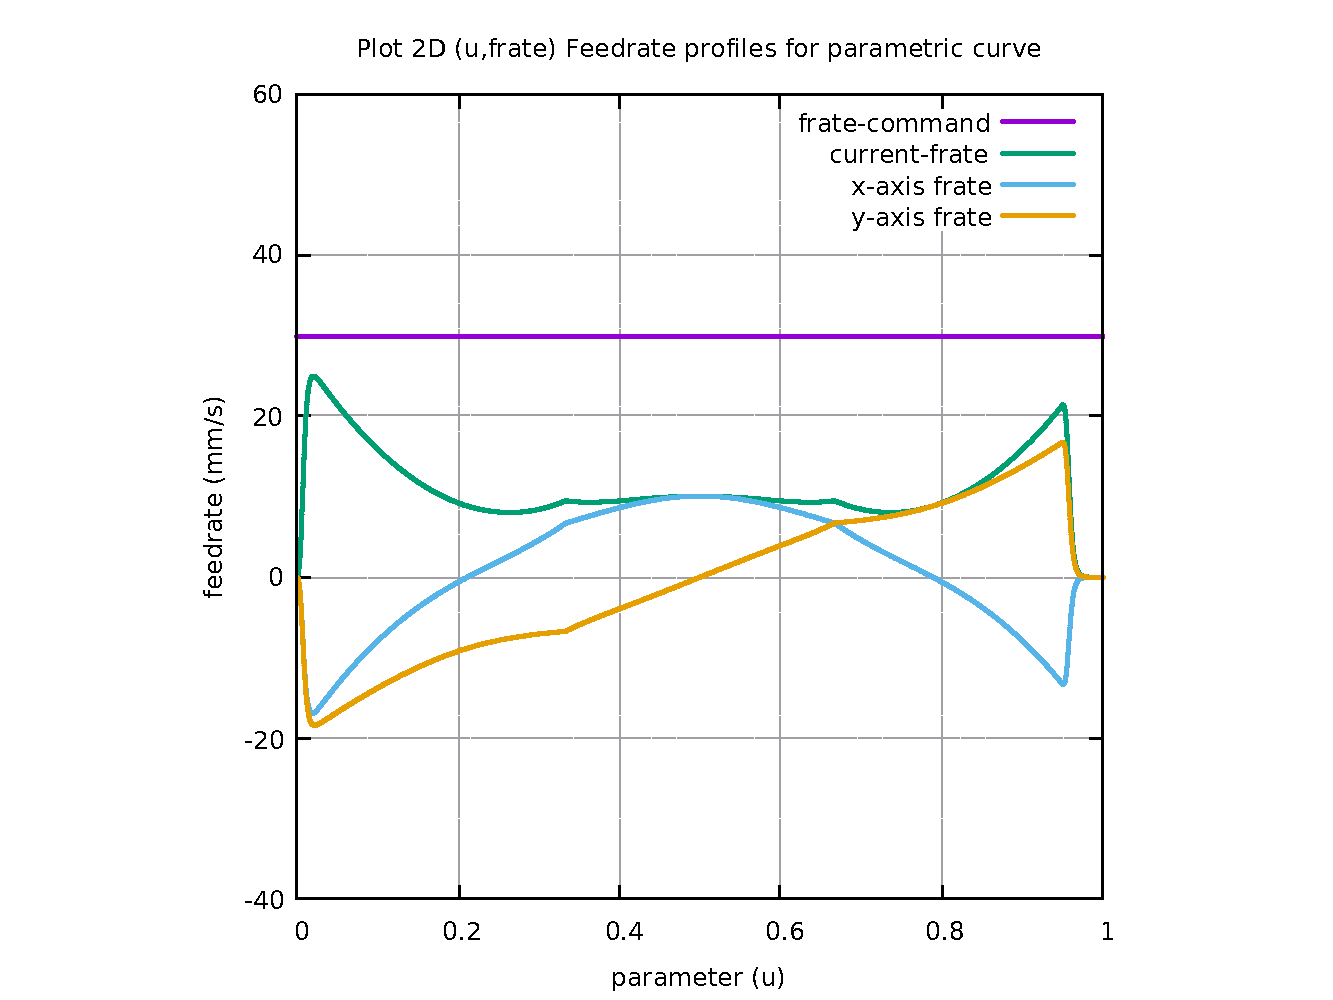
\includegraphics[width=0.90\textwidth]{Chap4/appendix/app-teardrop/img-Teardrop-FC30-Running-Feedrate-Profiles.pdf} }
\end{figure}	

\begin{figure}
	\caption  {Teardrop FC40 Running Feedrate Profiles}
	\label{img-chap4-Teardrop-FC40-Running-Feedrate-Profiles.pdf}
	%% \centering
	\framebox{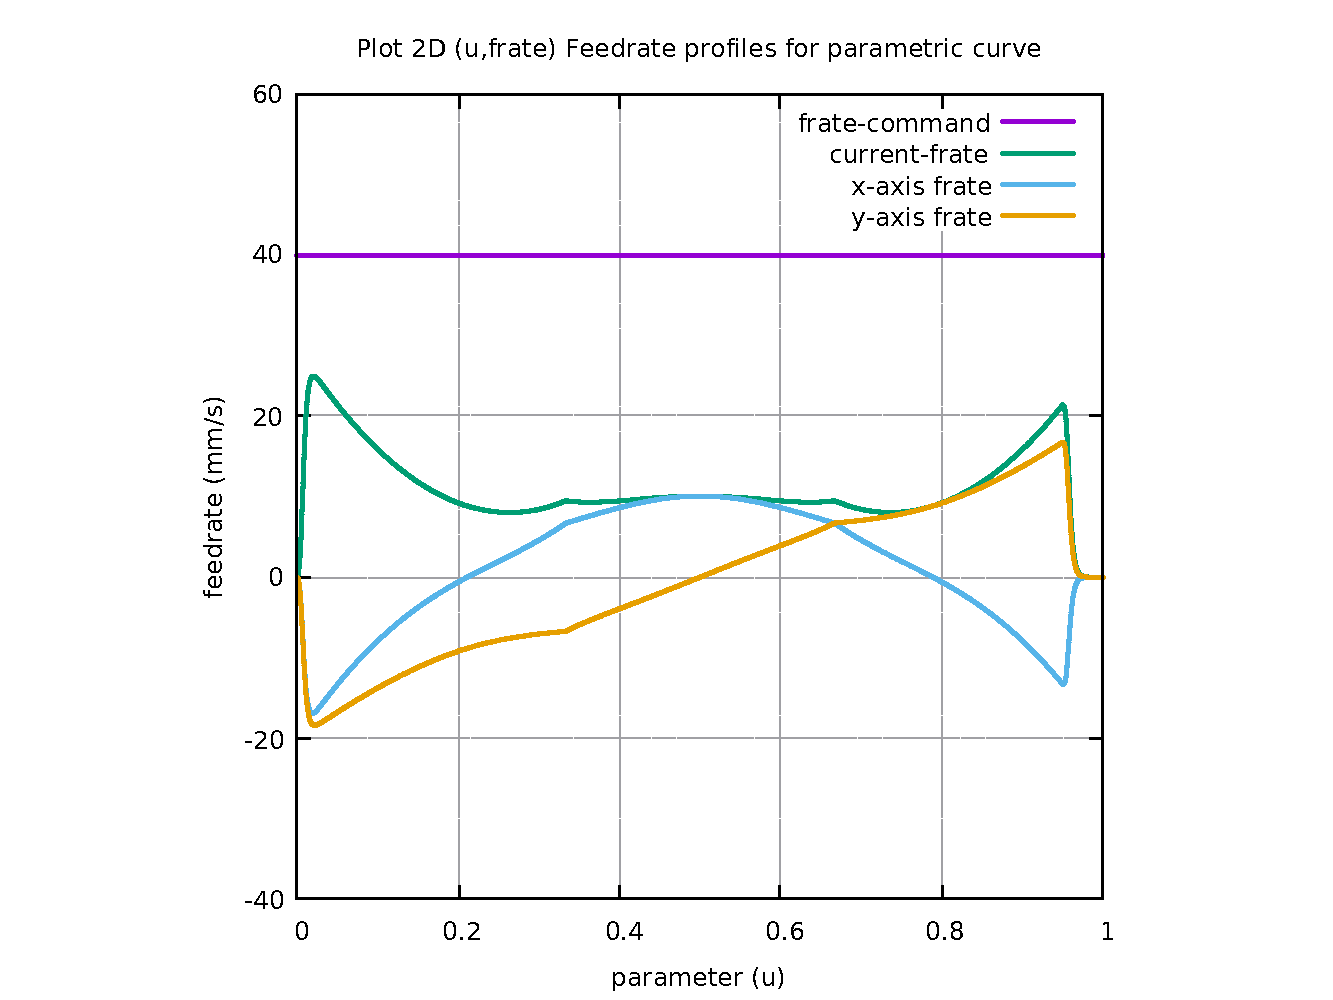
\includegraphics[width=0.90\textwidth]{Chap4/appendix/app-teardrop/img-Teardrop-FC40-Running-Feedrate-Profiles.pdf} }
\end{figure}	


%% ==================================================
\clearpage
\pagebreak

\subsection{Teardrop Color-coded Running Feedrates}
%% [\ref  {img-chap4-Teardrop FC10 Colored Feedrate Run Profile.pdf}] }
\label{ssec-chap4-Teardrop FC10 FC20 FC30 FC40 Colored Feedrate Run Profile}

In the next two(2) portrait pages, the Teardrop curve colored feedrate execution profiles for 
FC10 in Figure [\ref{img-chap4-Teardrop FC10 Colored Feedrate Run Profile}], 
FC20 in Figure [\ref{img-chap4-Teardrop FC20 Colored Feedrate Run Profile}], 
FC30 in Figure [\ref{img-chap4-Teardrop FC30 Colored Feedrate Run Profile}] and 
FC40 in Figure [\ref{img-chap4-Teardrop FC40 Colored Feedrate Run Profile}], 
respectively, are displayed. \\

The color spectrum legend on the right column for each curve was adjusted so that the maximum color code (red) represents the Feedrate Command FC for the particular run execution. This is the maximum value of the achievable running feedrate for each run. This setting provides more variations in colors along the curve path for each individual plot. Otherwise, the variations are not easily visible if the plots use a common maximum value for the color spectrum code.\\ 

As can be seen in all four(4) plots, the smoothness in running feedrates throughout the entire full curve path is shown by the linear and gradual transitions of colors (increasing or decreasing feedrates), that follow exactly the transitions in the color spectrum scale. Essentially, there are no sudden jump in colors. \\  

This smoothness requirement on running feedrate is one of the main objectives of the algorithm in this thesis.

%% PLOTS OF 4 COLORED FEEDRATES
%% ==============================================
\clearpage
\pagebreak 

\begin{figure}
	\caption  {Teardrop FC10 Colored Feedrate Run Profile}
	\label{img-chap4-Teardrop FC10 Colored Feedrate Run Profile}
	%% \centering
	\framebox{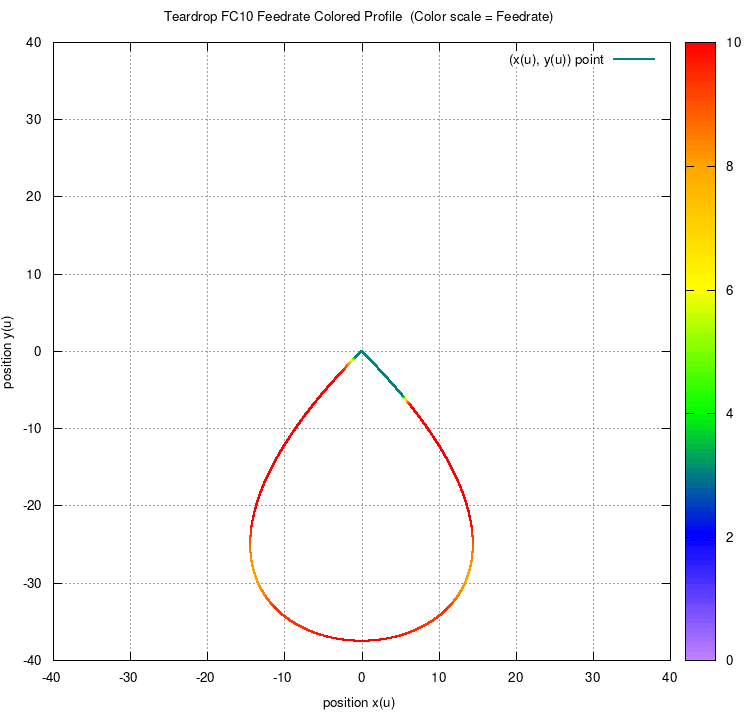
\includegraphics[width=0.73\textwidth]{Chap4/appendix/app-teardrop/TEARDROP-FC10-Colored-Feedrate-Profile-data_ngcode.png} }
\end{figure}	

\begin{figure}
	\caption  {Teardrop FC20 Colored Feedrate Run Profile}
	\label{img-chap4-Teardrop FC20 Colored Feedrate Run Profile}
	%% \centering
	\framebox{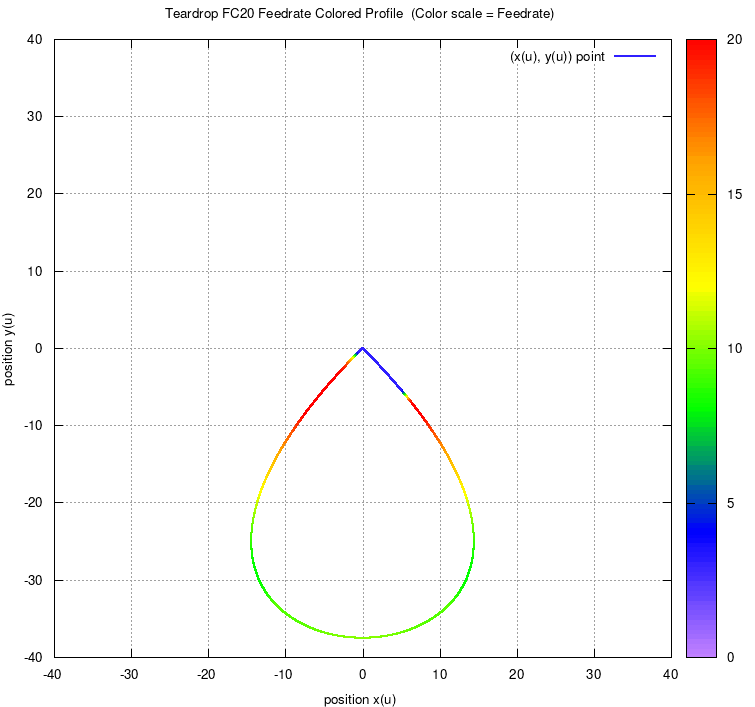
\includegraphics[width=0.73\textwidth]{Chap4/appendix/app-teardrop/TEARDROP-FC20-Colored-Feedrate-Profile-data_ngcode.png} }
\end{figure}	

%% ==================================================
\clearpage
\pagebreak

\begin{figure}
	\caption  {Teardrop FC30 Colored Feedrate Run Profile}
	\label{img-chap4-Teardrop FC30 Colored Feedrate Run Profile}
	%% \centering
	\framebox{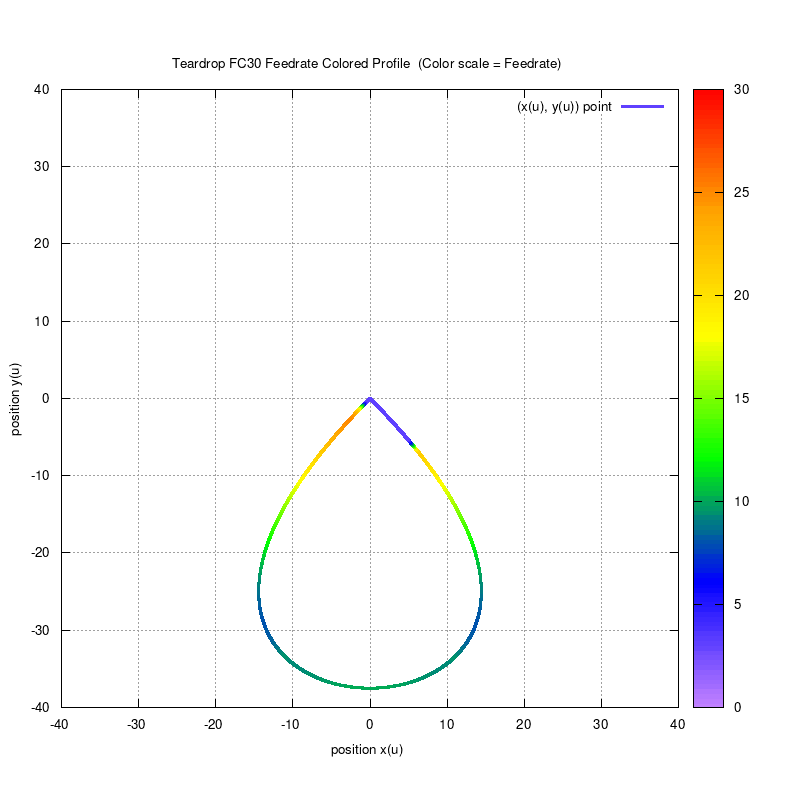
\includegraphics[width=0.73\textwidth]{Chap4/appendix/app-teardrop/TEARDROP-FC30-Colored-Feedrate-Profile-data_ngcode.png} }
\end{figure}	

\begin{figure}
	\caption  {Teardrop FC40 Colored Feedrate Run Profile}
	\label{img-chap4-Teardrop FC40 Colored Feedrate Run Profile}
	%% \centering
	\framebox{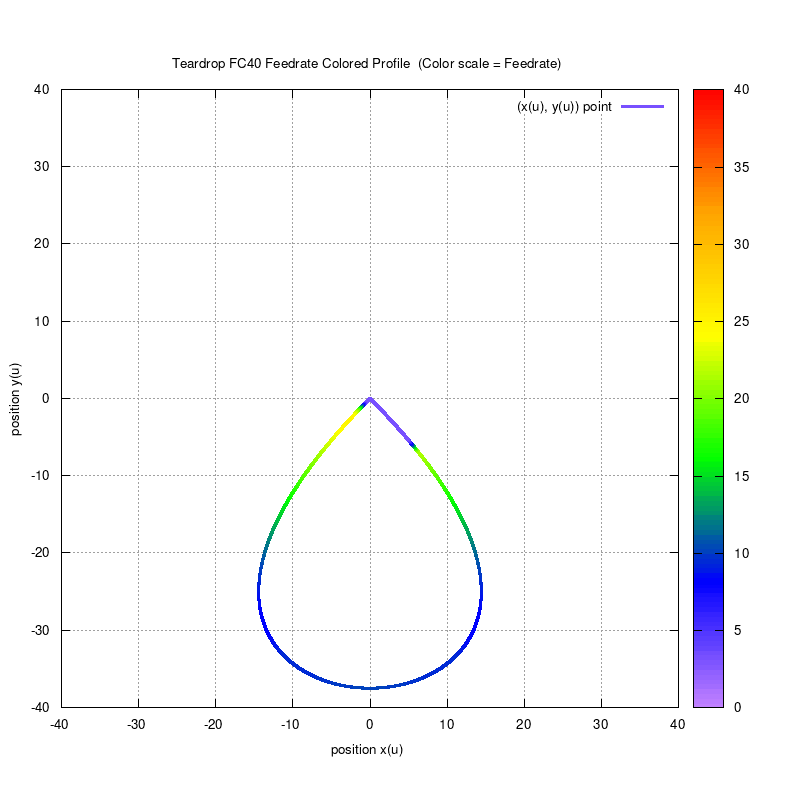
\includegraphics[width=0.73\textwidth]{Chap4/appendix/app-teardrop/TEARDROP-FC40-Colored-Feedrate-Profile-data_ngcode.png} }
\end{figure}	


%% ==============================================
\clearpage
\pagebreak

\subsection{Teardrop-Table FC 10, 20, 30 \& 40 Performance data}
%% [\ref  {tab-chap4-Teardrop-Table-FC10-20-30-40-Run-Performance-data.tex}] }
\label{ssec-chap4-Teardrop-Table-FC10-20-30-40-Run-Performance-data}

For the overall interpolation algorithm performance of the Teardrop curve, 20 different metrics were considered. The results are provided in Table [\ref{tab-chap4-Teardrop-Table-FC10-20-30-40-Run-Performance-data}], displayed in landscape mode.

The first three(3) rows of mandatory input parameters (Curve Type, Feedrate Command FC, and Lamda) uniquely identifies an execution run of the interpolation algorithm. The terms used in the data table are described as follows.\\

\begin{table}[ht]
%% \begin{center}
\caption{Terms used in Curve Performance data}
\label  {tab-chap4-Terms used in Curve Performance data}
%% IMPORTANT TO SCALEBOX BELOW
\scalebox{0.90}{
		
%% START COPY AND PASTE BELOW HERE
%% FROM \begin{tabular} UNTIL \end{tabular)
		
\begin{tabular}{ p{1.00cm} p{5.00cm} p{9.50cm} }
\hline
    &  & \\
TIP & Total Interpolated Points & Total number of points generated on the resulting curve by the interpolation algorithm for a complete run from u = 0.00 until u = 1.00.\\
    & & \\
SAL & Sum Arc Length     &  Sum of the arc-lengths accumulated as the parameter u is incremented to  u + (u-next). \\
    &                    & \\
SAT & Sum Arc Theta      &  Sum of the arc-theta angles in radians accumulated as the parameter u is incremented to u + (u-next). The arc-theta is the angle subtended by the arc segment between rho(u) and rho (u +(u-next)), where rho(u) is the Radius of Curvature at the point u. \\
    &                    & \\
SAA & Sum Arc Area       &  Sum of the arc-areas accumulated as the parameter u is incremented to  u + (u-next). The arc-area is the area bordered  by the chord from point u to  u + (u-next), and the corresponding arc segment.\\
    &                    & \\
SCL & Sum Chord Length   &  Sum of the chord-lengths accumulated as the parameter u is incremented to u + (u-next). \\
    &                    & \\
SCE & Sum Chord Error    &  Sum of the chord-errors accumulated as the parameter u is incremented to u + (u-next). \\
    & & \\
AAL & Average Arc Length   & AAL = (SAL)/(TIP-1) \\
AAT & Average Arc Theta    & AAT = (SAT)/(TIP-1)\\
AAA & Average Arc Area     & AAA = (SAA)/(TIP-1)\\
ACL & Average Chord Length & ACL = (SCL)/(TIP-1)\\
ACE & Average Chord Error  & ACE = (SCE)/(TIP-1)\\
    & & \\
RA1 & (SCE/TIP) & Sum Chord Error divided by Total Interpolated Points\\    
RA2 & (SCE/SCL) & Sum Chord Error divided by Sum Chord Length\\ 
RA2 & (SAA/SCL) & Sum Arc Area divided by Sum Chord Length\\ 
    &           &       
\end{tabular}

%% END COPY AND PASTE		

}   %% IMPORTANT FOR SCALEBOX CLOSING
\hrule
\end{table}

%% ==============================================
\clearpage
\pagebreak

Row (4) - Generally, as the Feedrate Command FC increases the number of Total Interpolated Points (TIP) decreases as expected. The last two columns FC30 and FC40 do not show reduction because the algorithm could not optimize constraints of chord-error and feedrate any further.\\

Row (5) - When the Feedrate Command FC increases, the Sum-Chord-Error (SCE) also increases. This is expected, since as FC increases, the chord-length increases, and with bigger (longer) chord-length the bigger the chord-error. \\

Row (6) - (SCE/TIP-1) which is Sum-Chord-Error divided by the number of chords for the entire length of the curve provides indicative comparison measures against the number of interpolated points for FC10, FC20, FC30 and FC40. \\

Rows (7) and (8) - These two rows, SAL and SCL, are interesting because SAL refers to the sum of arc-lengths while SCL refers to the sum of chord-lengths. The difference cannot be zero, no matter how small it is because of its geometrical definitions. SAL (arc-length) must always be greater than SCL (chord length) since individual chord lengths cannot be greater than its arc-length. If they are equal, then both are straight lines, and there is no arc segment anymore. \\

It is important to note that the calculation of the sum arc-length (SAL) in this work is just approximate. It is good for a circle because of the circle's perfect shape. For general curves, it is just a first-order approximation. In fact, a large body of work is involved in what is termed as "Near-Arc Approximation" for the calculation of the sum arc length (SAL). This method is not covered in this work. \\   

The special cases of the Circle and Ellipse curves, regarding SAL and SCL will be discussed separately in this Chapter 4, under section Notable Results Rest of Curves with reference link [\ref{Notable Results Rest of Curves}]. \\

Between SAL and SCL, the more reliable calculation is SCL, because the formula used for chord-length calculation (SCL) is exact. It is just the length of the line connecting two (x,y) points on the parametric curve. \\

Row (9) - The difference (SAL-SCL) must always be positive for all Feedrate Commands FC. However, for the Teardrop curve there is a negative result in column 3, for FC30. Similarly, this issue will be discussed further in this chapter, under section Notable Results Rest of Curves with reference link [\ref{Notable Results Rest of Curves}]. \\

Row (10) - The percentage difference (SAL-SCL)/SAL is important because it provides a value that is relative to its own size (length of curve). The difference (SAL - SCL) value alone is not meaningful because it varies differently for different curves. So percentage information is important because the comparison can be used against curves of different sizes (lengths).\\

Row (11) - This metric (SCE/SCL), which is the total sum of chord-errors divided by the total sum of chord-lengths, is the most meaningful measure of the efficiency or effectiveness of the algorithm developed in this work. This metric is general and not specific to any parametric curve. It is considered the performance measure for algorithm efficiency because it is independent of curve length. \\

The situation is analogous to comparing running speeds in meters per second. Whether you can run fast or not depends on your speed, and it does not matter how far or long you run. In the case of running it is about how many meters can you cover in one second. In the case of this work, it is about how much error does the algorithm generate per unit length of the curve traversed. \\

Row (12) and Row (13) - The meanings of Sum-Arc-Theta (SAT) and Sum-Arc-Area (SAA) are straightforward and self-explanatory. \\

Row (14) - This metric (SAA/SCL) or Sum Arc Area divided by the Sum Arc Length, carries the meaning similar to (SCE/SCL) in Row (11). However, the calculation of Arc-Area is approximate and not reliable for general curves, except for the Circle and Ellipse, which are perfect shapes. This is due to the fact that the Radius of Curvature rho(u), is used in the arc-area calculation. Similarly, this issue will be discussed further in this chapter, under section Notable Results Rest of Curves with reference link [\ref{Notable Results Rest of Curves}].\\

%% \clearpage
%% \pagebreak

Rows (15) to (19) - These rows are averages and they are self-explanatory. These averages provide valuable information when comparing among different parametric curves. This issue will be discussed further in this chapter, under section Overall Execution Results with reference link [\ref{sec-OVERALL EXECUTION RESULTS}].\\
 
Row (20) - This row Actual Runtime (ART), execution of the algorithm on the computer, measured is seconds, is just an indication (not exact measurements) regarding how many internal computing operations were carried out in FC10, FC20, FC30 and FC40 runs. Generally, algorithm runtime increases as the Feedrate Command FC increases.  It should be remembered that the algorithm performs recursive and iterative computations in order to constrain both chord-error and feedrate simultaneously. It means that the  higher the feedrate command, the more internal computations the algorithm has to perform.\\


%% TEARDROP TABLE DATA
%% ==============================================
\clearpage
\pagebreak
\begin{landscape}
	
\begin{table}[ht]
%% \begin{center}
\caption          {Teardrop Table FC10-20-30-40 Run Performance data}
\label  {tab-chap4-Teardrop-Table-FC10-20-30-40-Run-Performance-data}
%% IMPORTANT TO SCALEBOX BELOW
\scalebox{0.90}{
			
%% START COPY AND PASTE BELOW HERE
%% FROM \begin{tabular} UNTIL \end{tabular)
			
\begin{tabular}{ p{0.2cm} p{8.80cm} p{4.00cm} p{4.0cm} p{4.00cm} p{4.0cm}}
\hline
	&		&		&		&		&		\\
1	&	Curve Type	&	TEARDROP	&	TEARDROP	&	TEARDROP	&	TEARDROP	\\
2	&	User Feedrate Command FC(mm/s)                   	&	FC10	&	FC20	&	FC30	&	FC40	\\
3	&	User Lamda Acceleration Safety Factor	&	0.18	&	0.18	&	0.18	&	0.18	\\
&		&		&		&		&		\\
4	&	Total Iterpolated Points (TIP)	&	10261	&	7599	&	7347	&	7347	\\
5	&	Total Sum-Chord-Error (SCE) (mm)	&	5.809737838076E-03	&	7.140807162860E-03	&	7.336793707381E-03	&	7.335147000398E-03	\\
6	&	Ratio 1 = (SCE/TIP) = Chord-Error/Point	&	5.662512512745E-07	&	9.398272128007E-07	&	9.987467611463E-07	&	9.985225973861E-07	\\
&		&		&		&		&		\\
7	&	Total Sum-Arc-Length (SAL) (mm)	&	1.018356741269E+02	&	1.018418663504E+02	&	1.018595636256E+02	&	1.018355644559E+02	\\
8	&	Total Sum-Chord-Length (SCL) (mm)	&	1.018356732173E+02	&	1.018418655699E+02	&	1.018595666011E+02	&	1.018355608386E+02	\\
9	&	Difference = (SAL – SCL) (mm)	&	9.095903408252E-07	&	7.805327442156E-07	&	-2.975420997586E-06	&	3.617250541765E-06	\\
10	&	Percentage Difference = (SAL – SCL)/SAL	&	8.931942058845E-07	&	7.664163788301E-07	&	-2.921101261067E-06	&	3.552050367760E-06	\\
&		&		&		&		&		\\
11	&	Ratio 2 = (SCE/SCL) = Chord Error/Chord-Length	&	5.705012452441E-05	&	7.011661778683E-05	&	7.202851879506E-05	&	7.202932786929E-05	\\
&		&		&		&		&		\\
12	&	Total Sum-Arc-Theta (SAT) (rad)	&	4.712304324578E+00	&	4.712268805770E+00	&	4.712349787227E+00	&	4.712123379377E+00	\\
13	&	Total Sum-Arc-Area (SAA) (mm2)	&	3.822127588087E-05	&	6.182290957317E-05	&	6.781012634326E-05	&	6.777759239889E-05	\\
&		&		&		&		&		\\
14	&	Ratio 3 = (SAA/SCL) = Arc-Area/Chord-Length	&	5.705012452441E-05	&	7.011661778683E-05	&	7.202851879506E-05	&	7.202932786929E-05	\\
&		&		&		&		&		\\
15	&	Average-Chord-Error (ACE) (mm)	&	5.662512512745E-07	&	9.398272128007E-07	&	9.987467611463E-07	&	9.985225973861E-07	\\
16	&	Average-Arc-Length (AAL) (mm)	&	9.925504300871E-03	&	1.340377288107E-02	&	1.386599014779E-02	&	1.386272317668E-02	\\
17	&	Average-Chord-Length (ACL) (mm)	&	9.925504212216E-03	&	1.340377277834E-02	&	1.386599055283E-02	&	1.386272268427E-02	\\
18	&	Average-Arc-Theta (AAT) (rad)	&	4.592889205241E-04	&	6.201985793327E-04	&	6.414851330284E-04	&	6.414543124663E-04	\\
19	&	Average-Arc-Area (AAA) (mm2)	&	3.725270553691E-09	&	8.136734610840E-09	&	9.230891143923E-09	&	9.226462346704E-09	\\
&		&		&		&		&		\\
20	&	Algorithm actual runtime on computer (ART) (s) 	&	4.487434922	&	19.907344569	&	28.094412173	&	32.96324077	\\
&		&		&		&		&		


\end{tabular}
			
%% END COPY AND PASTE		
			
}   %% IMPORTANT FOR SCALEBOX CLOSING
\hrule
\end{table}
\end{landscape}

%% ==============================================
\clearpage
\pagebreak

\subsection{Teardrop Algorithm Performance and its metrics}
\label{ssec-chap4-Teardrop-Algorithm Performance}

The next four(4) portrait pages involve algorithm performance characteristics on the Teardrop curve. There are four(4) metrics developed to assess algorithm performance. The performance metrics for the Teardrop curve are described as follows.\\

%% \noindent
(1) Performance metric 1 (SCE/TIP) : This is the ratio of total sum-chord-error divided by the total number of interpolated points. The histogram plot is provided in Figure [\ref{img-chap4-Teardrop Run Performance 1: SCE/TIP}] and its corresponding data is provided in Table [\ref{tab-chap4-Teardrop-SCE/TIP Table-FC10-20-30-40-Run-Performance-data}]. This metric provides an impression on the average generated chord-error per chord. The number of chords is the Total Interpolated Points minus 1.\\

%% \noindent
(2) Performance metric 2 (SCE/SCL) : This is the ratio of total sum-chord-error divided by the total sum-chord-length. The histogram plot is provided in Figure [\ref{img-chap4-Teardrop Run Performance 2: SCE/SCL}] and its corresponding data is provided in Table [\ref{tab-chap4-Teardrop-SCE/SCL Table-FC10-20-30-40-Run-Performance-data}]. This metric accurately reflects the amount of chord-error generated per unit length of chord traversed. This the most useful and meaningful metric for the assessment of algorithm performance.\\
  
%% \noindent
(3) Performance metric 3 (SAA/SCL) : This is the ratio of the sum-arc-areas divided by the total sum-chord-length. The histogram plot is provided in Figure [\ref{img-chap4-Teardrop Run Performance 3: SAA/SCL}] and its corresponding data is provided in Table [\ref{tab-chap4-Teardrop-SAA/SCL Table-FC10-20-30-40-Run-Performance-data}]. This metric is useful and meaningful when the arc-area calculations are accurate, for example, in  cases of the circle and ellipse curves. For the rest, this metric is suspect due to the crude approximation in the arc-area calculation. \\

%% \noindent
(4) Performance metric 4 ((SAL-SCL)/SAL)*100 : This is the ratio of the difference between the sum-arc-length and the sum-chord-length, divided by the sum-arc-length and multiplied by 100 to represent it in percentage form. The histogram plot is provided in Figure [\ref{img-chap4-Teardrop Run Performance 4: 100*(SAL-SCL)/SAL}] and its corresponding data is provided in Table [\ref{tab-chap4-Teardrop-(SAL-SCL)/SAL Table-FC10-20-30-40-Run-Performance-data}]. For some of the curves where the calculation of arc-area is not reliable, this metric is not reliable.  

%% ==============================================
\clearpage
\pagebreak

%% HISTOGRAM

\begin{figure}
\caption  {Teardrop Run Performance 1: SCE/TIP}
\label{img-chap4-Teardrop Run Performance 1: SCE/TIP}
%% \centering
\framebox{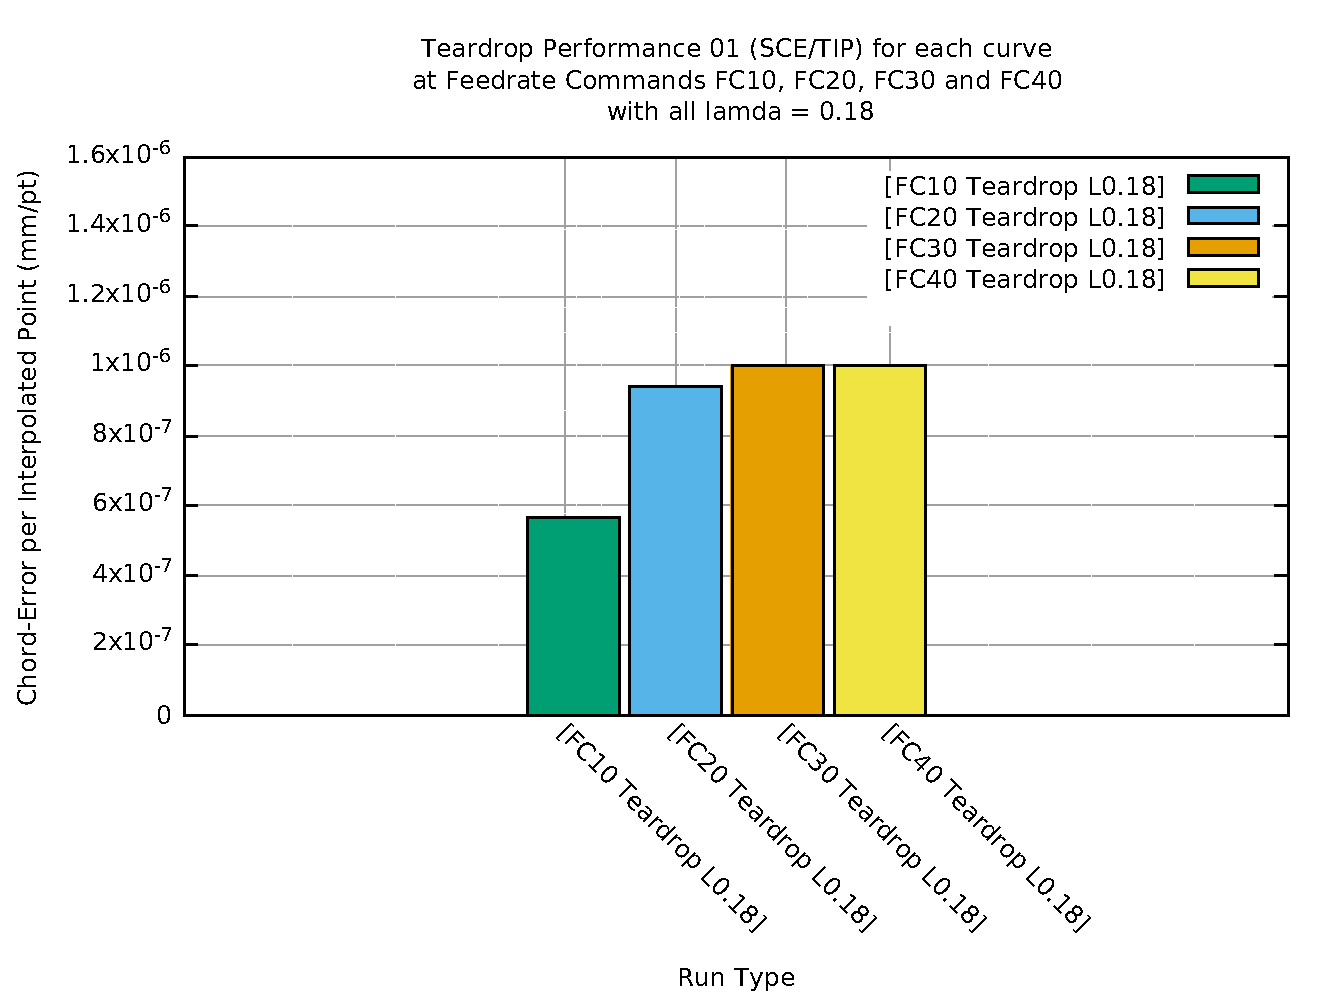
\includegraphics[width=1.00\textwidth]{Chap4/appendix/app-teardrop/HISTOGRAM/Teardrop-Performance-01-SCE-over-TIP.pdf}}
\end{figure}	

%% {Chap4/appendix/app-teardrop/HISTOGRAM/Teardrop-Performance-01-SCE-over-TIP.pdf}}

%% DATA TABLE
\begin{table}[ht]
%% \begin{center}
\caption{Teardrop SCE/TIP Table FC10-20-30-40 Run Performance data}
\label  {tab-chap4-Teardrop-SCE/TIP Table-FC10-20-30-40-Run-Performance-data}
%% IMPORTANT TO SCALEBOX BELOW
\scalebox{1.00}{
		
%% START COPY AND PASTE BELOW HERE
%% FROM \begin{tabular} UNTIL \end{tabular)
	
%% PORTRAIT 1.00 SCALEUP 14.00 cm WIDTH		
\begin{tabular}{ p{7.00cm} p{7.00cm} }
\hline
&		\\
Teardrop Performance 1: 	&	(SCE/TIP)	\\
Chord-Error per Interpolated-Point & \\
&		\\
FC10 Teardrop L0.18	&	5.662512512745E-07	\\
FC20 Teardrop L0.18	&	9.398272128007E-07	\\
FC30 Teardrop L0.18	&	9.987467611463E-07	\\
FC40 Teardrop L0.18	&	9.985225973861E-07	\\
&		
\end{tabular}

%% END COPY AND PASTE		
}   %% IMPORTANT FOR SCALEBOX CLOSING
\hrule
\end{table}

%% ====================================
\clearpage
\pagebreak
%% HISTOGRAM

\begin{figure}
\caption  {Teardrop Run Performance 2: SCE/SCL}
\label{img-chap4-Teardrop Run Performance 2: SCE/SCL}
%% \centering
\framebox{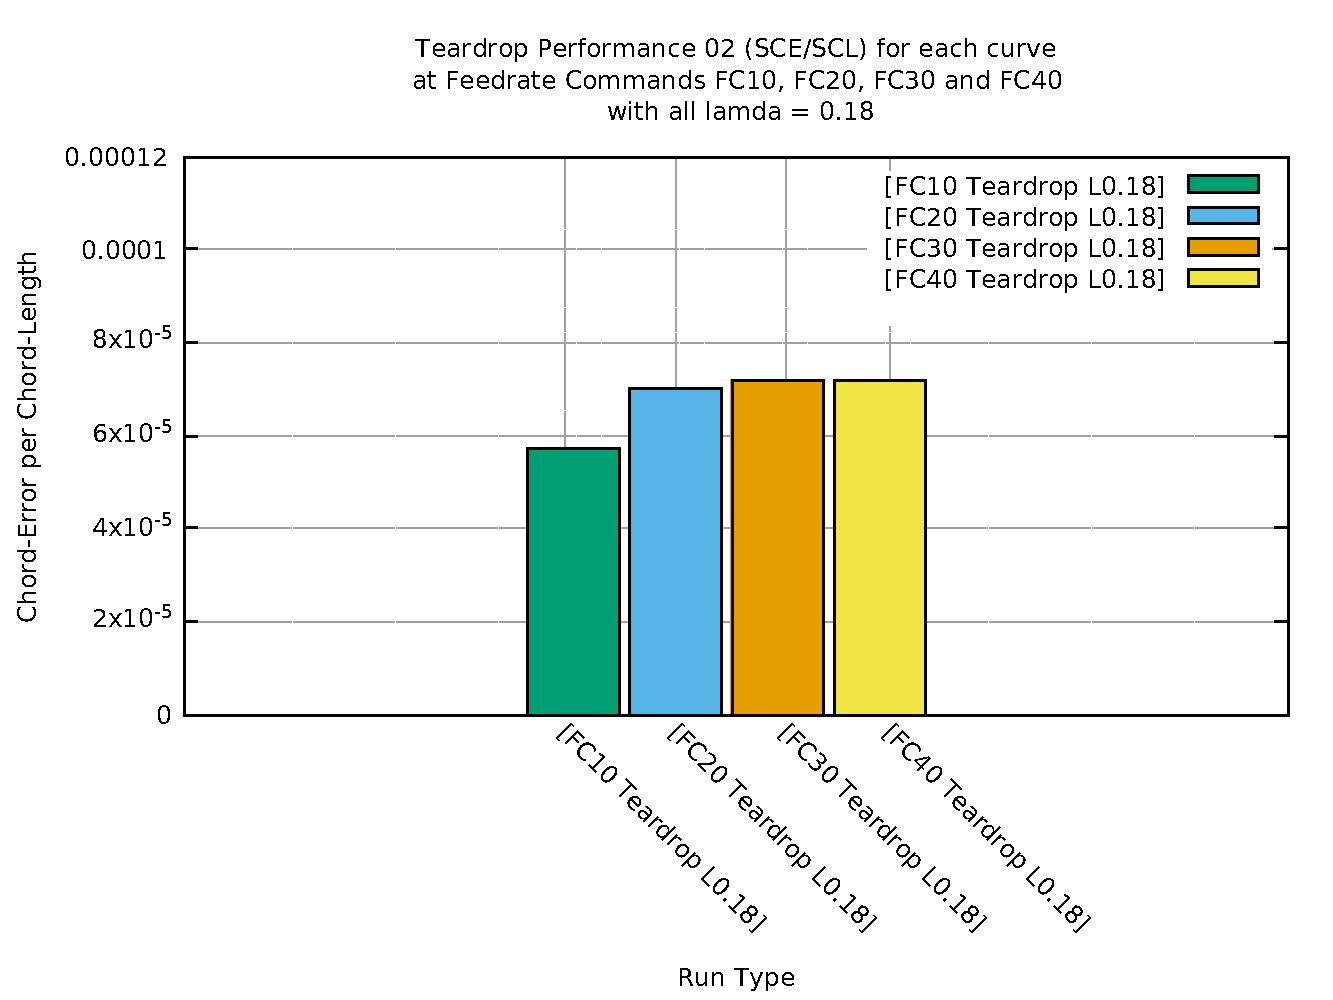
\includegraphics[width=1.00\textwidth]{Chap4/appendix/app-teardrop/HISTOGRAM/Teardrop-Performance-02-SCE-over-SCL.pdf}}
\end{figure}	


%% DATA TABLE
\begin{table}[ht]
%% \begin{center}
\caption{Teardrop SCE/SCL Table FC10-20-30-40 Run Performance data}
\label  {tab-chap4-Teardrop-SCE/SCL Table-FC10-20-30-40-Run-Performance-data}
%% IMPORTANT TO SCALEBOX BELOW
\scalebox{1.00}{
		
%% START COPY AND PASTE BELOW HERE
%% FROM \begin{tabular} UNTIL \end{tabular)

%% PORTRAIT 1.00 SCALEUP 14.00 cm WIDTH		
\begin{tabular}{ p{7.00cm} p{7.00cm} }
\hline
&		\\
Teardrop Performance 2: &	(SCE/SCL)	\\
Chord-Error per Chord-Length	& \\
&		\\
FC10 Teardrop L0.18	&	5.705012452441E-05	\\
FC20 Teardrop L0.18	&	7.011661778683E-05	\\
FC30 Teardrop L0.18	&	7.202851879506E-05	\\
FC40 Teardrop L0.18	&	7.202932786929E-05	\\
&		
\end{tabular}

%% END COPY AND PASTE		
}   %% IMPORTANT FOR SCALEBOX CLOSING
\hrule
\end{table}

%% ====================================
\clearpage
\pagebreak
%% HISTOGRAM

\begin{figure}
\caption  {Teardrop Run Performance 3: SAA/SCL}
\label{img-chap4-Teardrop Run Performance 3: SAA/SCL}
%% \centering
\framebox{\includegraphics[width=1.00\textwidth]{Chap4/appendix/app-teardrop/HISTOGRAM/Teardrop-Performance-03-SAA-over-SCL.pdf}}
\end{figure}	

%% DATA TABLE
\begin{table}[ht]
%% \begin{center}
\caption{Teardrop SAA/SCL Table FC10-20-30-40 Run Performance data}
\label  {tab-chap4-Teardrop-SAA/SCL Table-FC10-20-30-40-Run-Performance-data}
%% IMPORTANT TO SCALEBOX BELOW
\scalebox{1.00}{
		
%% START COPY AND PASTE BELOW HERE
%% FROM \begin{tabular} UNTIL \end{tabular)
		
%% PORTRAIT 1.00 SCALEUP 14.00 cm WIDTH		
\begin{tabular}{ p{7.00cm} p{7.00cm} }
\hline
&		\\
Teardrop Performance 3:	&	(SAA/SCL)	\\
Arc-Area per Chord-Length	& \\
&		\\
FC10 Teardrop L0.18	&	5.705012452441E-05	\\
FC20 Teardrop L0.18	&	7.011661778683E-05	\\
FC30 Teardrop L0.18	&	7.202851879506E-05	\\
FC40 Teardrop L0.18	&	7.202932786929E-05	\\
&		
\end{tabular}

%% END COPY AND PASTE		
}   %% IMPORTANT FOR SCALEBOX CLOSING
\hrule
\end{table}

%% ======================================
\clearpage
\pagebreak
%% HISTOGRAM

\begin{figure}
\caption  {Teardrop Run Performance 4: 100*(SAL-SCL)/SAL}
\label{img-chap4-Teardrop Run Performance 4: 100*(SAL-SCL)/SAL}
%% \centering
\framebox{\includegraphics[width=1.00\textwidth]{Chap4/appendix/app-teardrop/HISTOGRAM/Teardrop-Performance-04-Percentage-Difference-SAL-against-SCL.pdf}}
\end{figure}	

%% DATA TABLE
\begin{table}[ht]
%% \begin{center}
\caption{Teardrop (SAL-SCL)/SAL Table FC10-20-30-40 Run Performance data}
\label  {tab-chap4-Teardrop-(SAL-SCL)/SAL Table-FC10-20-30-40-Run-Performance-data}
%% IMPORTANT TO SCALEBOX BELOW
\scalebox{1.00}{
		
%% START COPY AND PASTE BELOW HERE
%% FROM \begin{tabular} UNTIL \end{tabular)
		
%% PORTRAIT 1.00 SCALEUP 14.00 cm WIDTH		
\begin{tabular}{ p{7.00cm} p{7.00cm} }
\hline
&		\\
Teardrop Percentage Difference :	&	(SAL-SCL)/(SAL)	\\
Arc-Length vs Chord-Length	& \\
&		\\
FC10 Teardrop L0.18	&	8.931942058845E-07	\\
FC20 Teardrop L0.18	&	7.664163788301E-07	\\
FC30 Teardrop L0.18	&	-2.921101261067E-06	\\
FC40 Teardrop L0.18	&	3.55205036776E-06	\\
&		
\end{tabular}

%% END COPY AND PASTE		
}   %% IMPORTANT FOR SCALEBOX CLOSING
\hrule
\end{table}

Negative values for this metric shall be discussed in this chapter, under section Notable Results Rest of Curves with reference link [\ref{Notable Results Rest of Curves}].\\


%% ==============================================
%% ==============================================
\clearpage
\pagebreak

\subsection{Teardrop Tangential Acceleration Run Profiles}
%% [\ref  {img-chap4-Teardrop FC10 Tangential Acceleration Run Profile.pdf}] }
\label{ssec-chap4-Teardrop FC10 Tangential Acceleration Run Profile}

In the next four(4) landscape pages, the Teardrop curve tangential acceleration $Tang\_Accn(u)$, execution profiles for 
FC10 in Figure [\ref{img-chap4-Teardrop FC10 Tangential Acceleration Run Profile}], 
FC20 in Figure [\ref{img-chap4-Teardrop FC20 Tangential Acceleration Run Profile}], 
FC30 in Figure [\ref{img-chap4-Teardrop FC30 Tangential Acceleration Run Profile}] and 
FC40 in Figure [\ref{img-chap4-Teardrop FC40 Tangential Acceleration Run Profile}], 
respectively, are displayed. \\

The CNC machine run parameters for the maximum acceleration settings is +30 mm/s2 for the x-axis direction, and also +30 mm/s2 for the y-axis direction. Similarly, the minimum settings are -30 mm/s2 for both the x and y axes, respectively. It is important to note here that negative means simply deceleration or decreasing feedrate.\\

\noindent
By Pythagoras Theorem, the maximum magnitude of the acceleration is:\\
$(Accn_{max} = sqrt( 30^{2} + 30^{2} )) = sqrt(1800) = 42.426$ mm/s2. \\
\noindent 
This is the value constraining the positive and negative accelerations in the ensuing plots. \\

\noindent
The algorithm execution results for the Teardrop curve at FC10, FC20, FC30 and FC40 in the next four(4) pages, show that the tangential acceleration upper and lower bounds \\
$(-42.426 \le Tang\_Accn(u) \le +42.426 )$ mm/s2, \\
\noindent
are not violated.\\

The "vertical drops and rises" seen in tangential acceleration profile are not actually sudden drops or rises since the number of interpolated points around these drops and rises are many, for example, an average of 600 points within delta-u = 0.10 throughout the full curve.  Upon closer inspection, as shown in Figure [\ref{img-chap4-Teardrop Closeup-View No Jitters FC40 Tangential Acceleration Run Profile}] for ranges $(0.333 \le u \le 0.335)$ and $(0.660 \le u \le 0.670)$, it is clear that these are not sudden drops or rises. This fact negates (denies) the occurrence of acceleration jitter.\\

The absolute confinement of tangential acceleration is one of the main objectives of the interpolation algorithm in this thesis.

%% LANDSCAPE PLOTS
%% ================
\clearpage
\pagebreak
\begin{landscape}
	
\begin{figure}
\caption  {      Teardrop Closeup-View No Jitters FC40 Tangential Acceleration Run Profile}
\label{img-chap4-Teardrop Closeup-View No Jitters FC40 Tangential Acceleration Run Profile}
\centering
\framebox{\includegraphics[width=1.30\textwidth]{Chap4/Curves/Teardrop/Teardrop-Close-up-view-NO-JITTERS.pdf}}
\end{figure}
	
\end{landscape}

%% ==================================================
\clearpage
\pagebreak
\begin{landscape}
	
	\begin{figure}
		\caption  {Teardrop FC10 Tangential Acceleration Run Profile}
		\label{img-chap4-Teardrop FC10 Tangential Acceleration Run Profile}
		\centering
		\framebox{\includegraphics[width=1.30\textwidth]{Chap4/appendix/app-teardrop/img-Teardrop-FC10-Tangential-Acceleration-Landscape.pdf} }
	\end{figure}
	
\end{landscape}

%% ==================================================
\clearpage
\pagebreak
\begin{landscape}
	
	\begin{figure}
		\caption  {Teardrop FC20 Tangential Acceleration Run Profile}
		\label{img-chap4-Teardrop FC20 Tangential Acceleration Run Profile}
		\centering
		\framebox{\includegraphics[width=1.30\textwidth]{Chap4/appendix/app-teardrop/img-Teardrop-FC20-Tangential-Acceleration-Landscape.pdf} }
	\end{figure}
	
\end{landscape}

%% ==================================================
\clearpage
\pagebreak
\begin{landscape}
	
	\begin{figure}
		\caption  {Teardrop FC30 Tangential Acceleration Run Profile}
		\label{img-chap4-Teardrop FC30 Tangential Acceleration Run Profile}
		\centering
		\framebox{\includegraphics[width=1.30\textwidth]{Chap4/appendix/app-teardrop/img-Teardrop-FC30-Tangential-Acceleration-Landscape.pdf} }
	\end{figure}
	
\end{landscape}

%% ==================================================
\clearpage
\pagebreak
\begin{landscape}
	
	\begin{figure}
		\caption  {Teardrop FC40 Tangential Acceleration Run Profile}
		\label{img-chap4-Teardrop FC40 Tangential Acceleration Run Profile}
		\centering
		\framebox{\includegraphics[width=1.30\textwidth]{Chap4/appendix/app-teardrop/img-Teardrop-FC40-Tangential-Acceleration-Landscape.pdf} }
	\end{figure}
	
\end{landscape}


%% ========================================================
%% ========================================================
\clearpage
\pagebreak
\section{PERFORMANCE SUMMARY REST OF CURVES} 
\label{Performance Summary Rest of Curves}

The performance summary data of the interpolation algorithm for the rest of curves (9 different curves) are provided in the next nine(9) pages in landscape mode. The respective links are provided below.

\subsection      {Circle-Table Summary Performance data link
[\ref  {tab-chap4-Circle-Table-FC10-20-30-40-Run-Performance-data}] }
\label{ssec-chap4-Circle-Table-FC10-20-30-40-Run-Performance-data}

\subsection      {Ellipse-Table Summary Performance data link
[\ref  {tab-chap4-Ellipse-Table-FC10-20-30-40-Run-Performance-data}] }
\label{ssec-chap4-Ellipse-Table-FC10-20-30-40-Run-Performance-data}

\subsection      {Butterfly-Table Summary Performance data link
[\ref  {tab-chap4-Butterfly-Table-FC10-20-30-40-Run-Performance-data}] }
\label{ssec-chap4-Butterfly-Table-FC10-20-30-40-Run-Performance-data}

\subsection      {Snailshell-Table Summary Performance data link
[\ref  {tab-chap4-Snailshell-Table-FC10-20-30-40-Run-Performance-data}] }
\label{ssec-chap4-Snailshell-Table-FC10-20-30-40-Run-Performance-data}

\subsection      {Skewed-Astroid-Table Summary Performance data link
[\ref  {tab-chap4-Skewed-Astroid-Table-FC10-20-30-40-Run-Performance-data}] }
\label{ssec-chap4-Skewed-Astroid-Table-FC10-20-30-40-Run-Performance-data}

\subsection      {Ribbon-10L-Table Summary Performance data link
[\ref  {tab-chap4-Ribbon-10L-Table-FC10-20-30-40-Run-Performance-data}] }
\label{ssec-chap4-Ribbon-10L-Table-FC10-20-30-40-Run-Performance-data}

\subsection      {Ribbon-100L-Table Summary Performance data link
[\ref  {tab-chap4-Ribbon-100L-Table-FC10-20-30-40-Run-Performance-data}] }
\label{ssec-chap4-Ribbon-100L-Table-FC10-20-30-40-Run-Performance-data}

\subsection      {AstEpi-Table Summary Performance data link
[\ref  {tab-chap4-AstEpi-Table-FC10-20-30-40-Run-Performance-data}] }
\label{ssec-chap4-AstEpi-Table-FC10-20-30-40-Run-Performance-data}

\subsection      {SnaHyp-Table Summary Performance data link
[\ref  {tab-chap4-SnaHyp-Table-FC10-20-30-40-Run-Performance-data}] }
\label{ssec-chap4-SnaHyp-Table-FC10-20-30-40-Run-Performance-data}

%% CIRCLE SUMMARY TABLE
%% ========================================================
\clearpage
\pagebreak
\begin{landscape}
	
\begin{table}[ht]
%% \begin{center}
\caption          {Circle Table FC10-20-30-40 Run Performance data}
\label  {tab-chap4-Circle-Table-FC10-20-30-40-Run-Performance-data}
%% IMPORTANT TO SCALEBOX BELOW
\scalebox{0.90}{
			
%% START COPY AND PASTE BELOW HERE
%% FROM \begin{tabular} UNTIL \end{tabular)
			
\begin{tabular}{ p{0.2cm} p{8.80cm} p{4.00cm} p{4.0cm} p{4.00cm} p{4.0cm}}
\hline
	&		&		&		&		&		\\
1	&	Curve Type	&	CIRCLE	&	CIRCLE	&	CIRCLE	&	CIRCLE	\\
2	&	User Feedrate Command FC(mm/s)                   	&	FC10	&	FC20	&	FC30	&	FC40	\\
3	&	User Lamda Acceleration Safety Factor	&	0.18	&	0.18	&	0.18	&	0.18	\\
&		&		&		&		&		\\
4	&	Total Iterpolated Points (TIP)	&	49641	&	24822	&	16549	&	12413	\\
5	&	Total Sum-Chord-Error (SCE) (mm)	&	1.093913738449E-03	&	2.187639876000E-03	&	3.281178287065E-03	&	4.374701201686E-03	\\
6	&	Ratio 1 = (SCE/TIP) = Chord-Error/Point	&	2.203694074232E-08	&	8.813665347893E-08	&	1.982824683989E-07	&	3.524573962041E-07	\\
&		&		&		&		&		\\
7	&	Total Sum-Arc-Length (SAL) (mm)	&	4.963785816452E+02	&	4.963771594934E+02	&	4.963757335444E+02	&	4.963942987341E+02	\\
8	&	Total Sum-Chord-Length (SCL) (mm)	&	4.963785813150E+02	&	4.963771581682E+02	&	4.963757305630E+02	&	4.963942934342E+02	\\
9	&	Difference = (SAL – SCL) (mm)	&	3.302195636934E-07	&	1.325165840171E-06	&	2.981455850204E-06	&	5.299917688717E-06	\\
10	&	Percentage Difference = (SAL – SCL)/SAL	&	6.652574786747E-08	&	2.669675295946E-07	&	6.006449648363E-07	&	1.067683029848E-06	\\
&		&		&		&		&		\\
11	&	Ratio 2 = (SCE/SCL) = Chord Error/Chord-Length	&	2.203789163406E-06	&	4.407213023407E-06	&	6.610271383220E-06	&	8.812956271960E-06	\\
&		&		&		&		&		\\
12	&	Total Sum-Arc-Theta (SAT) (rad)	&	6.283146611127E+00	&	6.283002050952E+00	&	6.282857458743E+00	&	6.282965934945E+00	\\
13	&	Total Sum-Arc-Area (SAA) (mm2)	&	5.235292684461E-05	&	2.093803820914E-04	&	4.710353817982E-04	&	8.373046676549E-04	\\
&		&		&		&		&		\\
14	&	Ratio 3 = (SAA/SCL) = Arc-Area/Chord-Length	&	2.203789163406E-06	&	4.407213023407E-06	&	6.610271383220E-06	&	8.812956271960E-06	\\
&		&		&		&		&		\\
15	&	Average-Chord-Error (ACE) (mm)	&	2.203694074232E-08	&	8.813665347893E-08	&	1.982824683989E-07	&	3.524573962041E-07	\\
16	&	Average-Arc-Length (AAL) (mm)	&	9.999568526293E-03	&	1.999827402173E-02	&	2.999611636116E-02	&	3.999309528956E-02	\\
17	&	Average-Chord-Length (ACL) (mm)	&	9.999568519641E-03	&	1.999827396834E-02	&	2.999611618099E-02	&	3.999309486257E-02	\\
18	&	Average-Arc-Theta (AAT) (rad)	&	1.265742669445E-04	&	2.531325108155E-04	&	3.796747316136E-04	&	5.062009293381E-04	\\
19	&	Average-Arc-Area (AAA) (mm2)	&	1.054652031519E-09	&	8.435614281914E-09	&	2.846479222856E-08	&	6.745928679140E-08	\\
&		&		&		&		&		\\
20	&	Algorithm actual runtime on computer (ART) (s) 	&	17.277667419	&	8.160163431	&	5.399371536	&	4.053925000	\\
&		&		&		&		&		

\end{tabular}

%% END COPY AND PASTE		
}   %% IMPORTANT FOR SCALEBOX CLOSING
\hrule
\end{table}
\end{landscape}

%% ELLIPSE SUMMARY TABLE
%% ========================================================
\clearpage
\pagebreak
\begin{landscape}
	
\begin{table}[ht]
%% \begin{center}
\caption          {Ellipse Table FC10-20-30-40 Run Performance data}
\label  {tab-chap4-Ellipse-Table-FC10-20-30-40-Run-Performance-data}
%% IMPORTANT TO SCALEBOX BELOW
\scalebox{0.90}{
			
%% START COPY AND PASTE BELOW HERE
%% FROM \begin{tabular} UNTIL \end{tabular)
			
\begin{tabular}{ p{0.2cm} p{8.80cm} p{4.00cm} p{4.0cm} p{4.00cm} p{4.0cm}}
\hline
	&		&		&		&		&		\\
1	&	Curve Type	&	ELLIPSE	&	ELLIPSE	&	ELLIPSE	&	ELLIPSE	\\
2	&	User Feedrate Command FC(mm/s)                   	&	FC10	&	FC20	&	FC30	&	FC40	\\
3	&	User Lamda Acceleration Safety Factor	&	0.18	&	0.18	&	0.18	&	0.18	\\
&		&		&		&		&		\\
4	&	Total Iterpolated Points (TIP)	&	21575	&	11296	&	8338	&	7351	\\
5	&	Total Sum-Chord-Error (SCE) (mm)	&	2.990951697698E-03	&	5.148661124856E-03	&	6.561982225601E-03	&	7.331840610025E-03	\\
6	&	Ratio 1 = (SCE/TIP) = Chord-Error/Point	&	1.386368637108E-07	&	4.558354249540E-07	&	7.870915467915E-07	&	9.975293346972E-07	\\
&		&		&		&		&		\\
7	&	Total Sum-Arc-Length (SAL) (mm)	&	2.156436635306E+02	&	2.156499394203E+02	&	2.156478495089E+02	&	2.156438658943E+02	\\
8	&	Total Sum-Chord-Length (SCL) (mm)	&	2.156436625529E+02	&	2.156499358521E+02	&	2.156478426167E+02	&	2.156438551446E+02	\\
9	&	Difference = (SAL – SCL) (mm)	&	9.777115224097E-07	&	3.568242959773E-06	&	6.892209597709E-06	&	1.074976646009E-05	\\
10	&	Percentage Difference = (SAL – SCL)/SAL	&	4.533921870933E-07	&	1.654645936542E-06	&	3.196048378596E-06	&	4.984962783667E-06	\\
&		&		&		&		&		\\
11	&	Ratio 2 = (SCE/SCL) = Chord Error/Chord-Length	&	1.386987988559E-05	&	2.387508767166E-05	&	3.042915776933E-05	&	3.399976598039E-05	\\
&		&		&		&		&		\\
12	&	Total Sum-Arc-Theta (SAT) (rad)	&	6.280515723261E+00	&	6.283169115421E+00	&	6.282291919271E+00	&	6.280610715483E+00	\\
13	&	Total Sum-Arc-Area (SAA) (mm2)	&	5.185017589366E-05	&	1.275076043292E-04	&	1.849039783361E-04	&	2.200267776119E-04	\\
&		&		&		&		&		\\
14	&	Ratio 3 = (SAA/SCL) = Arc-Area/Chord-Length	&	1.386987988559E-05	&	2.387508767166E-05	&	3.042915776933E-05	&	3.399976598039E-05	\\
&		&		&		&		&		\\
15	&	Average-Chord-Error (ACE) (mm)	&	1.386368637108E-07	&	4.558354249540E-07	&	7.870915467915E-07	&	9.975293346972E-07	\\
16	&	Average-Arc-Length (AAL) (mm)	&	9.995534603255E-03	&	1.909251345023E-02	&	2.586636074235E-02	&	2.933930148222E-02	\\
17	&	Average-Chord-Length (ACL) (mm)	&	9.995534557936E-03	&	1.909251313431E-02	&	2.586635991565E-02	&	2.933930001967E-02	\\
18	&	Average-Arc-Theta (AAT) (rad)	&	2.911150330611E-04	&	5.562788061462E-04	&	7.535434711852E-04	&	8.545048592494E-04	\\
19	&	Average-Arc-Area (AAA) (mm2)	&	2.403364044390E-09	&	1.128885385827E-08	&	2.217871876407E-08	&	2.993561600162E-08	\\
&		&		&		&		&		\\
20	&	Algorithm actual runtime on computer (ART) (s) 	&	7.13439876	&	7.633051722	&	11.041426063	&	16.776571251	\\
&		&		&		&		&		

\end{tabular}
			
%% END COPY AND PASTE		
}   %% IMPORTANT FOR SCALEBOX CLOSING
\hrule
\end{table}
\end{landscape}

%% BUTTERFLY SUMMARY TABLE
%% ========================================================
\clearpage
\pagebreak
\begin{landscape}
	
\begin{table}[ht]
%% \begin{center}
\caption          {Butterfly Table FC10-20-30-40 Run Performance data}
\label  {tab-chap4-Butterfly-Table-FC10-20-30-40-Run-Performance-data}
%% IMPORTANT TO SCALEBOX BELOW
\scalebox{0.90}{
			
%% START COPY AND PASTE BELOW HERE
%% FROM \begin{tabular} UNTIL \end{tabular)
			
\begin{tabular}{ p{0.2cm} p{8.80cm} p{4.00cm} p{4.0cm} p{4.00cm} p{4.0cm}}
\hline
	&		&		&		&		&		\\
1	&	Curve Type	&	BUTTERFLY	&	BUTTERFLY	&	BUTTERFLY	&	BUTTERFLY	\\
2	&	User Feedrate Command FC(mm/s)                   	&	FC10	&	FC20	&	FC30	&	FC40	\\
3	&	User Lamda Acceleration Safety Factor	&	0.18	&	0.18	&	0.18	&	0.18	\\
&		&		&		&		&		\\
4	&	Total Iterpolated Points (TIP)	&	35656	&	18029	&	12343	&	9732	\\
5	&	Total Sum-Chord-Error (SCE) (mm)	&	1.938859834664E-03	&	3.534046223178E-03	&	4.846582536157E-03	&	5.851472692902E-03	\\
6	&	Ratio 1 = (SCE/TIP) = Chord-Error/Point	&	5.437834342068E-08	&	1.960309642322E-07	&	3.926902071104E-07	&	6.013228540645E-07	\\
&		&		&		&		&		\\
7	&	Total Sum-Arc-Length (SAL) (mm)	&	3.560748506870E+02	&	3.560738974072E+02	&	3.560730284349E+02	&	3.560734306512E+02	\\
8	&	Total Sum-Chord-Length (SCL) (mm)	&	3.560747025702E+02	&	3.560737108999E+02	&	3.560727930088E+02	&	3.560731526728E+02	\\
9	&	Difference = (SAL – SCL) (mm)	&	1.481168304736E-04	&	1.865072539431E-04	&	2.354260789161E-04	&	2.779783607707E-04	\\
10	&	Percentage Difference = (SAL – SCL)/SAL	&	4.159710526812E-05	&	5.237880543932E-05	&	6.611735799000E-05	&	7.806770650153E-05	\\
&		&		&		&		&		\\
11	&	Ratio 2 = (SCE/SCL) = Chord Error/Chord-Length	&	5.445092899523E-06	&	9.925041122094E-06	&	1.361121273884E-05	&	1.643334424114E-05	\\
&		&		&		&		&		\\
12	&	Total Sum-Arc-Theta (SAT) (rad)	&	2.212404302532E+01	&	2.212055105865E+01	&	2.211618559661E+01	&	2.211929011631E+01	\\
13	&	Total Sum-Arc-Area (SAA) (mm2)	&	1.758667624644E-04	&	6.462621773264E-04	&	1.298932073590E-03	&	2.003665777961E-03	\\
&		&		&		&		&		\\
14	&	Ratio 3 = (SAA/SCL) = Arc-Area/Chord-Length	&	5.445092899523E-06	&	9.925041122094E-06	&	1.361121273884E-05	&	1.643334424114E-05	\\
&		&		&		&		&		\\
15	&	Average-Chord-Error (ACE) (mm)	&	5.437834342068E-08	&	1.960309642322E-07	&	3.926902071104E-07	&	6.013228540645E-07	\\
16	&	Average-Arc-Length (AAL) (mm)	&	9.986673697574E-03	&	1.975115916392E-02	&	2.885051275603E-02	&	3.659165868371E-02	\\
17	&	Average-Chord-Length (ACL) (mm)	&	9.986669543407E-03	&	1.975114881850E-02	&	2.885049368083E-02	&	3.659163011744E-02	\\
18	&	Average-Arc-Theta (AAT) (rad)	&	6.205032400874E-04	&	1.227010819761E-03	&	1.791945032946E-03	&	2.273074721643E-03	\\
19	&	Average-Arc-Area (AAA) (mm2)	&	4.932457228003E-09	&	3.584769122068E-08	&	1.052448609294E-07	&	2.059054339699E-07	\\
&		&		&		&		&		\\
20	&	Algorithm actual runtime on computer (ART) (s) 	&	14.219218872	&	8.1882168602	&	8.667691811	&	10.542664043	\\
&		&		&		&		&		

\end{tabular}
			
%% END COPY AND PASTE		
}   %% IMPORTANT FOR SCALEBOX CLOSING
\hrule
\end{table}
\end{landscape}

%% SNAILSHELL SUMMARY TABLE
%% ========================================================
\clearpage
\pagebreak
\begin{landscape}
	
\begin{table}[ht]
%% \begin{center}
\caption          {Snailshell Table FC10-20-30-40 Run Performance data}
\label  {tab-chap4-Snailshell-Table-FC10-20-30-40-Run-Performance-data}
%% IMPORTANT TO SCALEBOX BELOW
\scalebox{0.90}{
			
%% START COPY AND PASTE BELOW HERE
%% FROM \begin{tabular} UNTIL \end{tabular)
			
\begin{tabular}{ p{0.2cm} p{8.80cm} p{4.00cm} p{4.0cm} p{4.00cm} p{4.0cm}}
\hline
	&		&		&		&		&		\\
1	&	Curve Type	&	SNAILSHELL	&	SNAILSHELL	&	SNAILSHELL	&	SNAILSHELL	\\
2	&	User Feedrate Command FC(mm/s)                   	&	FC10	&	FC20	&	FC30	&	FC40	\\
3	&	User Lamda Acceleration Safety Factor	&	0.18	&	0.18	&	0.18	&	0.18	\\
&		&		&		&		&		\\
4	&	Total Iterpolated Points (TIP)	&	15621	&	9883	&	8370	&	7766	\\
5	&	Total Sum-Chord-Error (SCE) (mm)	&	5.115139395656E-03	&	6.269762299809E-03	&	6.764496555494E-03	&	7.045829082053E-03	\\
6	&	Ratio 1 = (SCE/TIP) = Chord-Error/Point	&	3.274737129101E-07	&	6.344628921078E-07	&	8.082801476275E-07	&	9.073830112110E-07	\\
&		&		&		&		&		\\
7	&	Total Sum-Arc-Length (SAL) (mm)	&	1.385725614787E+02	&	1.385823558880E+02	&	1.385855208343E+02	&	1.385878579474E+02	\\
8	&	Total Sum-Chord-Length (SCL) (mm)	&	1.385595406106E+02	&	1.385613905727E+02	&	1.385601641834E+02	&	1.385598862029E+02	\\
9	&	Difference = (SAL – SCL) (mm)	&	1.302086811782E-02	&	2.096531529295E-02	&	2.535665098060E-02	&	2.797174444973E-02	\\
10	&	Percentage Difference = (SAL – SCL)/SAL	&	9.396425943836E-03	&	1.512841599395E-02	&	1.829675338949E-02	&	2.018340196899E-02	\\
&		&		&		&		&		\\
11	&	Ratio 2 = (SCE/SCL) = Chord Error/Chord-Length	&	3.691654413053E-05	&	4.524898511695E-05	&	4.881992306637E-05	&	5.085042486059E-05	\\
&		&		&		&		&		\\
12	&	Total Sum-Arc-Theta (SAT) (rad)	&	1.894562150080E+01	&	1.894533592343E+01	&	1.894325318416E+01	&	1.894232057270E+01	\\
13	&	Total Sum-Arc-Area (SAA) (mm2)	&	1.070830851582E-04	&	3.068808285119E-04	&	5.164360050036E-04	&	7.283849492346E-04	\\
&		&		&		&		&		\\
14	&	Ratio 3 = (SAA/SCL) = Arc-Area/Chord-Length	&	3.691654413053E-05	&	4.524898511695E-05	&	4.881992306637E-05	&	5.085042486059E-05	\\
&		&		&		&		&		\\
15	&	Average-Chord-Error (ACE) (mm)	&	3.274737129101E-07	&	6.344628921078E-07	&	8.082801476275E-07	&	9.073830112110E-07	\\
16	&	Average-Arc-Length (AAL) (mm)	&	8.871482809134E-03	&	1.402371543089E-02	&	1.655938831812E-02	&	1.784776019928E-02	\\
17	&	Average-Chord-Length (ACL) (mm)	&	8.870649206822E-03	&	1.402159386488E-02	&	1.655635848768E-02	&	1.784415791409E-02	\\
18	&	Average-Arc-Theta (AAT) (rad)	&	1.212907906581E-03	&	1.917156033539E-03	&	2.263502591010E-03	&	2.439448882512E-03	\\
19	&	Average-Arc-Area (AAA) (mm2)	&	6.855511213715E-09	&	3.105452626107E-08	&	6.170820946393E-08	&	9.380359938629E-08	\\
&		&		&		&		&		\\
20	&	Algorithm actual runtime on computer (ART) (s) 	&	17.308275283	&	24.17500989	&	29.295160546	&	32.06253681	\\
&		&		&		&		&		

\end{tabular}
			
%% END COPY AND PASTE		
}   %% IMPORTANT FOR SCALEBOX CLOSING
\hrule
\end{table}
\end{landscape}

%% SKEWED-ASTROID SUMMARY TABLE
%% ========================================================
\clearpage
\pagebreak
\begin{landscape}
	
\begin{table}[ht]
%% \begin{center}
\caption          {Skewed-Astroid Table FC10-20-30-40 Run Performance data}
\label  {tab-chap4-Skewed-Astroid-Table-FC10-20-30-40-Run-Performance-data}
%% IMPORTANT TO SCALEBOX BELOW
\scalebox{0.90}{
			
%% START COPY AND PASTE BELOW HERE
%% FROM \begin{tabular} UNTIL \end{tabular)
			
\begin{tabular}{ p{0.2cm} p{8.80cm} p{4.00cm} p{4.0cm} p{4.00cm} p{4.0cm}}
\hline
	&		&		&		&		&		\\
1	&	Curve Type	&	SKEWED-ASTROID	&	SKEWED-ASTROID	&	SKEWED-ASTROID	&	SKEWED-ASTROID	\\
2	&	User Feedrate Command FC(mm/s)                   	&	FC10	&	FC20	&	FC30	&	FC40	\\
3	&	User Lamda Acceleration Safety Factor	&	0.18	&	0.18	&	0.18	&	0.18	\\
&		&		&		&		&		\\
4	&	Total Iterpolated Points (TIP)	&	116194	&	58102	&	38738	&	29056	\\
5	&	Total Sum-Chord-Error (SCE) (mm)	&	5.163683043374E-04	&	1.032591177038E-03	&	1.548668518105E-03	&	2.064600313211E-03	\\
6	&	Ratio 1 = (SCE/TIP) = Chord-Error/Point	&	4.444056908225E-09	&	1.777234775714E-08	&	3.997905150386E-08	&	7.105834841547E-08	\\
&		&		&		&		&		\\
7	&	Total Sum-Arc-Length (SAL) (mm)	&	1.161845691077E+03	&	1.161851349542E+03	&	1.161856975395E+03	&	1.161862568638E+03	\\
8	&	Total Sum-Chord-Length (SCL) (mm)	&	4.457142858819E+02	&	4.457142855374E+02	&	4.457142846207E+02	&	4.457142831748E+02	\\
9	&	Difference = (SAL – SCL) (mm)	&	7.161314051951E+02	&	7.161370640044E+02	&	7.161426907744E+02	&	7.161482854628E+02	\\
10	&	Percentage Difference = (SAL – SCL)/SAL	&	6.163739390653E+01	&	6.163758077028E+01	&	6.163776660469E+01	&	6.163795140613E+01	\\
&		&		&		&		&		\\
11	&	Ratio 2 = (SCE/SCL) = Chord Error/Chord-Length	&	1.158518631091E-06	&	2.316710975042E-06	&	3.474576811966E-06	&	4.632116113725E-06	\\
&		&		&		&		&		\\
12	&	Total Sum-Arc-Theta (SAT) (rad)	&	8.421542473789E+00	&	8.421464824576E+00	&	8.421387277982E+00	&	8.421309770499E+00	\\
13	&	Total Sum-Arc-Area (SAA) (mm2)	&	4.343191363991E-05	&	1.736583480748E-04	&	3.905753943512E-04	&	6.940792041172E-04	\\
&		&		&		&		&		\\
14	&	Ratio 3 = (SAA/SCL) = Arc-Area/Chord-Length	&	1.158518631091E-06	&	2.316710975042E-06	&	3.474576811966E-06	&	4.632116113725E-06	\\
&		&		&		&		&		\\
15	&	Average-Chord-Error (ACE) (mm)	&	4.444056908225E-09	&	1.777234775714E-08	&	3.997905150386E-08	&	7.105834841547E-08	\\
16	&	Average-Arc-Length (AAL) (mm)	&	9.999274406178E-03	&	1.999709728820E-02	&	2.999346814144E-02	&	3.998838646145E-02	\\
17	&	Average-Chord-Length (ACL) (mm)	&	3.835982252648E-03	&	7.671370295474E-03	&	1.150616425177E-02	&	1.534036424625E-02	\\
18	&	Average-Arc-Theta (AAT) (rad)	&	7.247891416685E-05	&	1.449452647042E-04	&	2.173990571800E-04	&	2.898402949750E-04	\\
19	&	Average-Arc-Area (AAA) (mm2)	&	3.737911375032E-10	&	2.988904632878E-09	&	1.008274761471E-08	&	2.388845995929E-08	\\
&		&		&		&		&		\\
20	&	Algorithm actual runtime on computer (ART) (s) 	&	38.427006969	&	19.305250287	&	12.910301226	&	9.663656563	\\
&		&		&		&		&		

\end{tabular}
			
%% END COPY AND PASTE		
}   %% IMPORTANT FOR SCALEBOX CLOSING
\hrule
\end{table}
\end{landscape}

%% RIBBON-10L SUMMARY TABLE
%% ========================================================
\clearpage
\pagebreak
\begin{landscape}
	
\begin{table}[ht]
%% \begin{center}
\caption          {Ribbon-10L Table FC10-20-30-40 Run Performance data}
\label  {tab-chap4-Ribbon-10L-Table-FC10-20-30-40-Run-Performance-data}
%% IMPORTANT TO SCALEBOX BELOW
\scalebox{0.90}{
			
%% START COPY AND PASTE BELOW HERE
%% FROM \begin{tabular} UNTIL \end{tabular)
			
\begin{tabular}{ p{0.2cm} p{8.80cm} p{4.00cm} p{4.0cm} p{4.00cm} p{4.0cm}}
\hline
	&		&		&		&		&		\\
1	&	Curve Type	&	RIBBON-10L	&	RIBBON-10L	&	RIBBON-10L	&	RIBBON-10L	\\
2	&	User Feedrate Command FC(mm/s)                   	&	FC10	&	FC20	&	FC30	&	FC40	\\
3	&	User Lamda Acceleration Safety Factor	&	0.18	&	0.18	&	0.18	&	0.18	\\
&		&		&		&		&		\\
4	&	Total Iterpolated Points (TIP)	&	7351	&	7352	&	7353	&	7353	\\
5	&	Total Sum-Chord-Error (SCE) (mm)	&	7.331686925442E-03	&	7.330650001960E-03	&	7.330843544266E-03	&	7.330107781796E-03	\\
6	&	Ratio 1 = (SCE/TIP) = Chord-Error/Point	&	9.975084252302E-07	&	9.972316694273E-07	&	9.971223536814E-07	&	9.970222771758E-07	\\
&		&		&		&		&		\\
7	&	Total Sum-Arc-Length (SAL) (mm)	&	3.802699021307E+00	&	3.802672335504E+00	&	3.803478267930E+00	&	3.802978777888E+00	\\
8	&	Total Sum-Chord-Length (SCL) (mm)	&	1.521079586306E+01	&	1.521068903483E+01	&	1.521391385441E+01	&	1.521191524702E+01	\\
9	&	Difference = (SAL – SCL) (mm)	&	-1.140809684176E+01	&	-1.140801669932E+01	&	-1.141043558648E+01	&	-1.140893646914E+01	\\
10	&	Percentage Difference = (SAL – SCL)/SAL	&	-2.999999941577E+02	&	-2.999999919218E+02	&	-3.000000205782E+02	&	-3.000000035623E+02	\\
&		&		&		&		&		\\
11	&	Ratio 2 = (SCE/SCL) = Chord Error/Chord-Length	&	4.820054776519E-04	&	4.819406921788E-04	&	4.818512589475E-04	&	4.818661991448E-04	\\
&		&		&		&		&		\\
12	&	Total Sum-Arc-Theta (SAT) (rad)	&	5.446619853644E+00	&	5.446616685362E+00	&	5.446717935311E+00	&	5.446655391021E+00	\\
13	&	Total Sum-Arc-Area (SAA) (mm2)	&	1.338515095667E-06	&	1.338121185915E-06	&	1.338217831316E-06	&	1.337920946871E-06	\\
&		&		&		&		&		\\
14	&	Ratio 3 = (SAA/SCL) = Arc-Area/Chord-Length	&	4.820054776519E-04	&	4.819406921788E-04	&	4.818512589475E-04	&	4.818661991448E-04	\\
&		&		&		&		&		\\
15	&	Average-Chord-Error (ACE) (mm)	&	9.975084252302E-07	&	9.972316694273E-07	&	9.971223536814E-07	&	9.970222771758E-07	\\
16	&	Average-Arc-Length (AAL) (mm)	&	5.173740165044E-04	&	5.173000048298E-04	&	5.173392638643E-04	&	5.172713245223E-04	\\
17	&	Average-Chord-Length (ACL) (mm)	&	2.069496035791E-03	&	2.069199977531E-03	&	2.069357161916E-03	&	2.069085316516E-03	\\
18	&	Average-Arc-Theta (AAT) (rad)	&	7.410367147815E-04	&	7.409354761749E-04	&	7.408484678062E-04	&	7.408399606938E-04	\\
19	&	Average-Arc-Area (AAA) (mm2)	&	1.821108973696E-10	&	1.820325378744E-10	&	1.820209237372E-10	&	1.819805422838E-10	\\
&		&		&		&		&		\\
20	&	Algorithm actual runtime on computer (ART) (s) 	&	65.683135834	&	59.539855092	&	75.452534184	&	73.307374778	\\
&		&		&		&		&		

\end{tabular}
			
%% END COPY AND PASTE		
}   %% IMPORTANT FOR SCALEBOX CLOSING
\hrule
\end{table}
\end{landscape}

%% RIBBON-100L SUMMARY TABLE
%% ========================================================
\clearpage
\pagebreak
\begin{landscape}
	
\begin{table}[ht]
%% \begin{center}
\caption          {Ribbon-100L Table FC10-20-30-40 Run Performance data}
\label  {tab-chap4-Ribbon-100L-Table-FC10-20-30-40-Run-Performance-data}
%% IMPORTANT TO SCALEBOX BELOW
\scalebox{0.90}{
			
%% START COPY AND PASTE BELOW HERE
%% FROM \begin{tabular} UNTIL \end{tabular)
			
\begin{tabular}{ p{0.2cm} p{8.80cm} p{4.00cm} p{4.0cm} p{4.00cm} p{4.0cm}}
\hline
	&		&		&		&		&		\\
1	&	Curve Type	&	RIBBON-100L	&	RIBBON-100L	&	RIBBON-100L	&	RIBBON-100L	\\
2	&	User Feedrate Command FC(mm/s)                   	&	FC10	&	FC20	&	FC30	&	FC40	\\
3	&	User Lamda Acceleration Safety Factor	&	0.18	&	0.18	&	0.18	&	0.18	\\
&		&		&		&		&		\\
4	&	Total Iterpolated Points (TIP)	&	7480	&	7348	&	7349	&	7350	\\
5	&	Total Sum-Chord-Error (SCE) (mm)	&	7.227413654822E-03	&	7.334488978808E-03	&	7.333764811636E-03	&	7.333839687707E-03	\\
6	&	Ratio 1 = (SCE/TIP) = Chord-Error/Point	&	9.663609646773E-07	&	9.982971251951E-07	&	9.980627125254E-07	&	9.979370918094E-07	\\
&		&		&		&		&		\\
7	&	Total Sum-Arc-Length (SAL) (mm)	&	3.802433940498E+01	&	3.802572368417E+01	&	3.802757758292E+01	&	3.803483632374E+01	\\
8	&	Total Sum-Chord-Length (SCL) (mm)	&	1.520973548479E+02	&	1.521028906780E+02	&	1.521103086280E+02	&	1.521393532475E+02	\\
9	&	Difference = (SAL – SCL) (mm)	&	-1.140730154429E+02	&	-1.140771669938E+02	&	-1.140827310451E+02	&	-1.141045169238E+02	\\
10	&	Percentage Difference = (SAL – SCL)/SAL	&	-2.999999927099E+02	&	-2.999999893265E+02	&	-2.999999955199E+02	&	-3.000000209086E+02	\\
&		&		&		&		&		\\
11	&	Ratio 2 = (SCE/SCL) = Chord Error/Chord-Length	&	4.751833890898E-05	&	4.822057586226E-05	&	4.821346349097E-05	&	4.820475130965E-05	\\
&		&		&		&		&		\\
12	&	Total Sum-Arc-Theta (SAT) (rad)	&	5.446630718238E+00	&	5.446603832206E+00	&	5.446627300213E+00	&	5.446718506955E+00	\\
13	&	Total Sum-Arc-Area (SAA) (mm2)	&	1.265139232664E-04	&	1.339597112819E-04	&	1.339309239988E-04	&	1.339343540720E-04	\\
&		&		&		&		&		\\
14	&	Ratio 3 = (SAA/SCL) = Arc-Area/Chord-Length	&	4.751833890898E-05	&	4.822057586226E-05	&	4.821346349097E-05	&	4.820475130965E-05	\\
&		&		&		&		&		\\
15	&	Average-Chord-Error (ACE) (mm)	&	9.663609646773E-07	&	9.982971251951E-07	&	9.980627125254E-07	&	9.979370918094E-07	\\
16	&	Average-Arc-Length (AAL) (mm)	&	5.084147533759E-03	&	5.175680370787E-03	&	5.175228304698E-03	&	5.175511814362E-03	\\
17	&	Average-Chord-Length (ACL) (mm)	&	2.033658976439E-02	&	2.070272093072E-02	&	2.070091298694E-02	&	2.070204833957E-02	\\
18	&	Average-Arc-Theta (AAT) (rad)	&	7.282565474312E-04	&	7.413371215743E-04	&	7.412394257230E-04	&	7.411509738679E-04	\\
19	&	Average-Arc-Area (AAA) (mm2)	&	1.691588758743E-08	&	1.823325320292E-08	&	1.822685410980E-08	&	1.822484066840E-08	\\
&		&		&		&		&		\\
20	&	Algorithm actual runtime on computer (ART) (s) 	&	26.306206937	&	37.694118593	&	42.698734839	&	47.339581162	\\
&		&		&		&		&		

\end{tabular}
			
%% END COPY AND PASTE		
}   %% IMPORTANT FOR SCALEBOX CLOSING
\hrule
\end{table}
\end{landscape}

%% ASTEPI SUMMARY TABLE
%% ========================================================
\clearpage
\pagebreak
\begin{landscape}
	
\begin{table}[ht]
%% \begin{center}
\caption          {AstEpi Table FC10-20-30-40 Run Performance data}
\label  {tab-chap4-AstEpi-Table-FC10-20-30-40-Run-Performance-data}
%% IMPORTANT TO SCALEBOX BELOW
\scalebox{0.90}{
			
%% START COPY AND PASTE BELOW HERE
%% FROM \begin{tabular} UNTIL \end{tabular)
			
\begin{tabular}{ p{0.2cm} p{8.80cm} p{4.00cm} p{4.0cm} p{4.00cm} p{4.0cm}}
\hline
	&		&		&		&		&		\\
1	&	Curve Type	&	ASTEPI	&	ASTEPI	&	ASTEPI	&	ASTEPI	\\
2	&	User Feedrate Command FC(mm/s)                   	&	FC10	&	FC20	&	FC30	&	FC40	\\
3	&	User Lamda Acceleration Safety Factor	&	0.18	&	0.18	&	0.18	&	0.18	\\
&		&		&		&		&		\\
4	&	Total Iterpolated Points (TIP)	&	76275	&	38169	&	25499	&	19184	\\
5	&	Total Sum-Chord-Error (SCE) (mm)	&	8.403732211685E-04	&	1.641842648547E-03	&	2.390002467065E-03	&	3.111370462905E-03	\\
6	&	Ratio 1 = (SCE/TIP) = Chord-Error/Point	&	1.101782024240E-08	&	4.301620856599E-08	&	9.373293854673E-08	&	1.621941543505E-07	\\
&		&		&		&		&		\\
7	&	Total Sum-Arc-Length (SAL) (mm)	&	7.626471894183E+02	&	7.626564180797E+02	&	7.626597716718E+02	&	7.626830175974E+02	\\
8	&	Total Sum-Chord-Length (SCL) (mm)	&	4.262622478423E+02	&	4.262622396899E+02	&	4.262622295515E+02	&	4.262622333550E+02	\\
9	&	Difference = (SAL – SCL) (mm)	&	3.363849415760E+02	&	3.363941783897E+02	&	3.363975421203E+02	&	3.364207842424E+02	\\
10	&	Percentage Difference = (SAL – SCL)/SAL	&	4.410754359858E+01	&	4.410822100426E+01	&	4.410846810274E+01	&	4.411017113009E+01	\\
&		&		&		&		&		\\
11	&	Ratio 2 = (SCE/SCL) = Chord Error/Chord-Length	&	1.971493430212E-06	&	3.851719659103E-06	&	5.606883043752E-06	&	7.299193359018E-06	\\
&		&		&		&		&		\\
12	&	Total Sum-Arc-Theta (SAT) (rad)	&	1.300410711943E+01	&	1.300415390419E+01	&	1.300401093322E+01	&	1.300396323193E+01	\\
13	&	Total Sum-Arc-Area (SAA) (mm2)	&	2.898515736808E-04	&	6.811935608835E-04	&	9.367445601128E-04	&	1.255001527807E-03	\\
&		&		&		&		&		\\
14	&	Ratio 3 = (SAA/SCL) = Arc-Area/Chord-Length	&	1.971493430212E-06	&	3.851719659103E-06	&	5.606883043752E-06	&	7.299193359018E-06	\\
&		&		&		&		&		\\
15	&	Average-Chord-Error (ACE) (mm)	&	1.101782024240E-08	&	4.301620856599E-08	&	9.373293854673E-08	&	1.621941543505E-07	\\
16	&	Average-Arc-Length (AAL) (mm)	&	9.998783195037E-03	&	1.998156618318E-02	&	2.991057226731E-02	&	3.975827647383E-02	\\
17	&	Average-Chord-Length (ACL) (mm)	&	5.588565537959E-03	&	1.116805281099E-02	&	1.671747703944E-02	&	2.222083268285E-02	\\
18	&	Average-Arc-Theta (AAT) (rad)	&	1.704920040831E-04	&	3.407082871566E-04	&	5.100012131627E-04	&	6.778899667376E-04	\\
19	&	Average-Arc-Area (AAA) (mm2)	&	3.800136005465E-09	&	1.784724273956E-08	&	3.673796219754E-08	&	6.542258915741E-08	\\
&		&		&		&		&		\\
20	&	Algorithm actual runtime on computer (ART) (s) 	&	27.836373672	&	14.372286925	&	9.138001576	&	7.71877336	\\
&		&		&		&		&		

\end{tabular}
			
%% END COPY AND PASTE		
}   %% IMPORTANT FOR SCALEBOX CLOSING
\hrule
\end{table}
\end{landscape}

%% SNAHYP SUMMARY TABLE
%% ========================================================
\clearpage
\pagebreak
\begin{landscape}
	
\begin{table}[ht]
%% \begin{center}
\caption          {SnaHyp Table FC10-20-30-40 Run Performance data}
\label  {tab-chap4-SnaHyp-Table-FC10-20-30-40-Run-Performance-data}
%% IMPORTANT TO SCALEBOX BELOW
\scalebox{0.90}{
			
%% START COPY AND PASTE BELOW HERE
%% FROM \begin{tabular} UNTIL \end{tabular)
			
\begin{tabular}{ p{0.2cm} p{8.80cm} p{4.00cm} p{4.0cm} p{4.00cm} p{4.0cm}}
\hline
	&		&		&		&		&		\\
1	&	Curve Type	&	SNAHYP	&	SNAHYP	&	SNAHYP	&	SNAHYP	\\
2	&	User Feedrate Command FC(mm/s)                   	&	FC10	&	FC20	&	FC25*	&	FC28**	\\
3	&	User Lamda Acceleration Safety Factor	&	0.18	&	0.18	&	0.18	&	0.18	\\
&		&		&		&		&		\\
4	&	Total Iterpolated Points (TIP)	&	38672	&	20223	&	16618	&	15102	\\
5	&	Total Sum-Chord-Error (SCE) (mm)	&	2.846873175820E-03	&	4.002975369043E-03	&	4.459254922025E-03	&	4.700022719935E-03	\\
6	&	Ratio 1 = (SCE/TIP) = Chord-Error/Point	&	7.361778014067E-08	&	1.979515067275E-07	&	2.683549932012E-07	&	3.112391709116E-07	\\
&		&		&		&		&		\\
7	&	Total Sum-Arc-Length (SAL) (mm)	&	3.779474877648E+02	&	3.779592539969E+02	&	3.779667959094E+02	&	3.779678653378E+02	\\
8	&	Total Sum-Chord-Length (SCL) (mm)	&	4.789870865777E+02	&	4.789986994127E+02	&	4.790063715425E+02	&	4.790071286890E+02	\\
9	&	Difference = (SAL – SCL) (mm)	&	-1.010395988129E+02	&	-1.010394454158E+02	&	-1.010395756332E+02	&	-1.010392633512E+02	\\
10	&	Percentage Difference = (SAL – SCL)/SAL	&	-2.673376648446E+01	&	-2.673289365118E+01	&	-2.673239467770E+01	&	-2.673223641934E+01	\\
&		&		&		&		&		\\
11	&	Ratio 2 = (SCE/SCL) = Chord Error/Chord-Length	&	5.943528031539E-06	&	8.356965006276E-06	&	9.309385400583E-06	&	9.812009964860E-06	\\
&		&		&		&		&		\\
12	&	Total Sum-Arc-Theta (SAT) (rad)	&	5.483921922253E+02	&	5.514331568816E+02	&	5.514225232921E+02	&	5.481728747328E+02	\\
13	&	Total Sum-Arc-Area (SAA) (mm2)	&	2.706870610425E-01	&	2.760007501922E-01	&	2.777614243305E-01	&	2.754368695310E-01	\\
&		&		&		&		&		\\
14	&	Ratio 3 = (SAA/SCL) = Arc-Area/Chord-Length	&	5.943528031539E-06	&	8.356965006276E-06	&	9.309385400583E-06	&	9.812009964860E-06	\\
&		&		&		&		&		\\
15	&	Average-Chord-Error (ACE) (mm)	&	7.361778014067E-08	&	1.979515067275E-07	&	2.683549932012E-07	&	3.112391709116E-07	\\
16	&	Average-Arc-Length (AAL) (mm)	&	9.773408698114E-03	&	1.869049817016E-02	&	2.274579020939E-02	&	2.502932688814E-02	\\
17	&	Average-Chord-Length (ACL) (mm)	&	1.238620895704E-02	&	2.368700916886E-02	&	2.882628462072E-02	&	3.172022572604E-02	\\
18	&	Average-Arc-Theta (AAT) (rad)	&	1.418096744913E-02	&	2.726897225208E-02	&	3.318424043402E-02	&	3.630043538393E-02	\\
19	&	Average-Arc-Area (AAA) (mm2)	&	6.999742986798E-06	&	1.364853872971E-05	&	1.671549764280E-05	&	1.823964436336E-05	\\
&		&		&		&		&		\\
20	&	Algorithm actual runtime on computer (ART) (s) 	&	18.694644926	&	16.525007035	&	16.49022576	&	16.65385009	\\
&		&		&		&		&		

\end{tabular}
			
%% END COPY AND PASTE		
}   %% IMPORTANT FOR SCALEBOX CLOSING
\hrule
\end{table}
\end{landscape}


%% ========================================================
%% ========================================================
\clearpage
\pagebreak
\section{NOTABLE RESULTS REST OF CURVES} 
\label{Notable Results Rest of Curves}

\subsection{Algorithm validation and verification of Circle curve}
\label{ssec-Algorithm validation and verification of Circle curve}

Using PI = 3.14159\_26535\_89793\_238 at (18-decimal digits in precision), the circumference of the Circle with radius R = 79.0 in this work is equal to 2*PI*R = 4.963716392672E+02. The total angle subtended by the circle in radians is 2*PI = 6.283185307180E+00. For comparisons, the results calculated by the algorithm extracted from Circle Table [\ref  {tab-chap4-Circle-Table-FC10-20-30-40-Run-Performance-data}], in rows (7, 8, and 12), are provided in the table below.

\begin{table}[ht]
%% \begin{center}
\caption          {Circle - Algorithm Validation and Verification}
\label  {tab-chap4-Circle - Algorithm Validation and Verification}
%% IMPORTANT TO SCALEBOX BELOW
\scalebox{0.90}{
		
%% START COPY AND PASTE BELOW HERE
%% FROM \begin{tabular} UNTIL \end{tabular)
		
\begin{tabular}{ p{0.2cm} p{8.80cm} p{4.00cm} }
\hline
  &                              & \\
  & CIRCUMFERENCE CIRCLE (mm)    & \\
1 & Mathematical Formula         & 4.963716392672E+02 \\
&                          & \\
& SUM-ARC-LENGTH (SAL)     & \\
2 & SAL FC10-Circle-L0.18    & 4.963785816452E+02  \\
3 & SAL FC20-Circle-L0.18    & 4.963771594934E+02  \\
4 & SAL FC30-Circle-L0.18    & 4.963757335444E+02  \\
5 & SAL FC40-Circle-L0.18    & 4.963942987341E+02  \\
&                            & \\
& SUM-CHORD-LENGTH (SAL)     & \\                         
6 & SCL FC10-Circle-L0.18    & 4.963785813150E+02  \\
7 & SCL FC20-Circle-L0.18    & 4.963771581682E+02  \\
8 & SCL FC30-Circle-L0.18    & 4.963757305630E+02  \\
9 & SCL FC40-Circle-L0.18    & 4.963942934342E+02  \\                         
&                             & \\
& FULL ANGLE CIRCLE  (rad)    & \\
10 & Mathematical Formula     & 6.283185307180E+00 \\
&                             & \\
& SUM-ARC-THETA (SAT)         & \\
11 & SAT FC10-Circle-L0.18    & 6.283146611127E+00  \\
12 & SAT FC20-Circle-L0.18    & 6.283002050952E+00  \\
13 & SAT FC30-Circle-L0.18    & 6.282857458743E+00  \\
14 & SAT FC40-Circle-L0.18    & 6.282965934945E+00  \\    			
   &                          & 
\end{tabular}
		
%% END COPY AND PASTE		
}   %% IMPORTANT FOR SCALEBOX CLOSING
\hrule
\end{table}

From the results in the table above, it can be seen that values calculated by the algorithm are in very good agreement (up to 4 decimal places) with results calculated using mathematical formulas. It is said that the Circle curve validates and verifies the algorithm. In reverse, it can also be said that the algorithm validates and verifies the Circle curve. By definition, the sum-chord-lengths (SCL) must always be lower that the sum-arc-lengths (SAL). This fact is evident in the table above.


%% =====================================
\clearpage
\pagebreak

\subsection{Algorithm validation and verification of Ellipse curve}
\label{ssec-Algorithm validation and verification of Ellipse curve}

For the Ellipse curve that is origin centered and elongated along the y-axis, the length of the semi-minor axis a, is the value of x when y= 0.00. Similarly, the length of the semi-major axis b, is the value of y when x= 0.00. \\

The perimeter of the Ellipse curve is calculated using the Ramanujan approximation formula shown in Appendix-Chap4 [\ref{app-chap4-Ellipse Perimeter using Ramanujan Approximation}] with the lengths of semi-minor axis a = 11.0 and semi-major axis b = 51.0, respectively. The result for the Ellipse perimeter calculation is 2.156404170793E+02. For a simple closed figure like the Ellipse, the total angle subtended (SAT) by the curve at the center in radians is 2*PI = 6.283185307180E+00. \\

As comparisons, the results calculated by the algorithm extracted from Ellipse Table [\ref{tab-chap4-Ellipse-Table-FC10-20-30-40-Run-Performance-data}], in rows (7, 8, and 12), are provided in the table below. \\

\begin{table}[ht]
%% \begin{center}
\caption          {Ellipse - Algorithm Validation and Verification}
\label  {tab-chap4-Ellipse - Algorithm Validation and Verification}
%% IMPORTANT TO SCALEBOX BELOW
\scalebox{0.90}{
		
%% START COPY AND PASTE BELOW HERE
%% FROM \begin{tabular} UNTIL \end{tabular)
		
\begin{tabular}{ p{0.2cm} p{8.80cm} p{4.00cm} }
\hline
  &                           & \\
  & PERIMETER ELLIPSE (mm)    & \\
1 & Mathematical Formula      & 2.156404170793E+02 \\
&                             & \\
& SUM-ARC-LENGTH (SAL)        & \\
2 & SAL FC10-Ellipse-L0.18    & 2.156436635306E+02  \\
3 & SAL FC20-Ellipse-L0.18    & 2.156499394203E+02  \\
4 & SAL FC30-Ellipse-L0.18    & 2.156478495089E+02  \\
5 & SAL FC40-Ellipse-L0.18    & 2.156438658943E+02  \\
&                             & \\
& SUM-CHORD-LENGTH (SAL)      & \\                         
6 & SCL FC10-Ellipse-L0.18    &  2.156436625529E+02 \\
7 & SCL FC20-Ellipse-L0.18    &  2.156499358521E+02 \\
8 & SCL FC30-Ellipse-L0.18    &  2.156478426167E+02 \\
9 & SCL FC40-Ellipse-L0.18    &  2.156438551446E+02 \\                         
&                             & \\
& FULL ANGLE CIRCLE  (rad)    & \\
10 & Mathematical Formula     & 6.283185307180E+00 \\
&                             & \\
& SUM-ARC-THETA (SAT)         & \\
11 & SAT FC10-Ellipse-L0.18   & 6.280515723261E+00  \\
12 & SAT FC20-Ellipse-L0.18   & 6.283169115421E+00  \\
13 & SAT FC30-Ellipse-L0.18   & 6.282291919271E+00  \\
14 & SAT FC40-Ellipse-L0.18   & 6.280610715483E+00  \\         
   &                          & 
\end{tabular}
		
%% END COPY AND PASTE		
}   %% IMPORTANT FOR SCALEBOX CLOSING
\hrule
\end{table}

From the results in the table above, it can be seen that values calculated by the algorithm are in very good agreement (up to 4 decimal places) with results calculated using mathematical formulas. It is said that the Ellipse curve validates and verifies the algorithm. In reverse, it can also be said that the algorithm validates and verifies the Ellipse curve. By definition, the sum-chord-lengths (SCL) must always be lower that the sum-arc-lengths (SAL). This fact is evident in the table above.


%% =====================================
\clearpage
\pagebreak

\subsection{Case Sum-Arc-Length (SAL) less than Sum-Chord-Length (SCL)}
\label{ssec-Case Total Sum-Arc-Length SAL less than Total Sum-Chord-Length SCL}

The case where the Total Sum-Arc-Length (SAL) is less than Total Sum-Chord-Length (SCL) is abnormal and considered rogue. It should be the opposite or reverse. The values of SAL should always be greater than SCL. \\

The following table (in landscape mode) is an extract of data from the Teardrop Table [\ref{tab-chap4-Teardrop-Table-FC10-20-30-40-Run-Performance-data}], from rows (7, 8, 9 and 10), showing an abnormal case. Notice that the anomaly or abnormality happens only for FC30, the third row, and not for FC10, FC20 and FC40. The summary results of algorithm re-executions (as checks) of the Teardrop curve at FC10, FC20, FC30 and FC40 are provided in Listing [\ref{lst-Anomaly Run FC30 Teardrop L0.18}] on the next page. There is a negative difference for (SAL-SCL) in FC30.\\


Figure [\ref{img-chap4-Plot of Teardrop FC10 FC20 FC30 and FC40 Differences SAL-SCL}], presents four(4) different curves the of Teardrop Differences (SAL-SCL), for FC10, FC20, FC30 and FC40, all running at a commom Lamda = 0.18. However, only 3 curves are visible. The last curve is actually an overlap of FC30 and FC40 curves. The difference is so small that it is not visible at the current plot scale. The next Figure [\ref{img-chap4-Teardrop Separation of FC30 and FC40 Difference SAL-SCL}], for clarity shows FC30 and FC40 separation by shifting the left scale higher by 0.01 mm relative to the right scale. \\

The next Figure [\ref{img-chap4-Plot of Teardrop Overlap FC30 and FC40 Differences SAL-SCL}], shows both FC30 and FC40 on the same x and y-axes scales, displaying an apparent overlap. However, upon taking a closeup view as in Figure [\ref{img-chap4-Teardrop Separation Closeup of FC30 and FC40 Difference SAL-SCL}], of a specific region $(0.48 \le u \le 0.52)$, and zooming in the y-axis, the separation becomes evident. The actual values for FC30 and FC40 are different, having a very small gap in the order of $1E-5$, and both are positive.  \\    

The positiveness of both SAL and SCL throughout the full parameter range $(0.00 \le u \le 1.00)$, can be seen through NAL (next-arc-length) and NCL (next-chord-length), in the next four(4) figures, namely Figure [\ref{img-chap4-Plot of Teardrop FC10 NAL and NCL}], [\ref{img-chap4-Plot of Teardrop FC20 NAL and NCL}], [\ref{img-chap4-Plot of Teardrop FC30 NAL and NCL}] and [\ref{img-chap4-Plot of Teardrop FC40 NAL and NCL}], for FC10, FC20, FC30 and FC40, respectively. The left and right y-axes scales have been shifted by 0.01 mm relative to each other, in order to separate NAL(u) and NCL(u), which otherwise shows an apparent overlap. \\ 




Since NAL(k) and NCL(k) are all positive throughout $(0.00 \le k \le 1.00)$, which is the entire parametric curve, the Total SAL and Total NCL must also be both positive. Therefore, a negative difference between Total SAL and Total SCL, is not a problem. It just means that, for the particular case, the value of Total SCL calculated by the algorithm is higher than Total SAL. That is the explanation. \\

Why? Again it is about FC30 or Feedrate Command 30 mm/s that is having problems. And remember that the maximum machine limit for velocity is 30 mm/s for the x-axis direction, and also 30 mm/s for the y-axis direction. That means the algorithm is running at exactly the maximum allowable limits, and this may have led the approximate first-order arc length calculation into problems. \\

Notice that the same algorithm for the arc length calculation does not have problems for FC10, FC20 and FC40. These are feedrate commands that are out of the machine velocity limits. If FC30 is the threshold, above which the algorithm encounters negative difference problems, then it would not be correct for FC40, where there is no such negative difference. So FC30 is not a threshold point, and in this case it is just an anomaly. \\

The (SAL - SCL) negative difference anomalies are also found in algorithm executions for the Ribbon-10L link [\ref  {tab-chap4-Ribbon-10L-Table-FC10-20-30-40-Run-Performance-data}], Ribbon-100L link [\ref  {tab-chap4-Ribbon-100L-Table-FC10-20-30-40-Run-Performance-data}], and SnaHyp [\ref{tab-chap4-SnaHyp-Table-FC10-20-30-40-Run-Performance-data}], curves. This just means the approximation equation used in calculating the arc-lengths is inferior (as reminded earlier) to the formula for calculating the chord-lengths.    


%% ========================================================
\clearpage
\pagebreak
\begin{landscape}
	
	\begin{table}[ht]
		%% \begin{center}
		\caption          {Anomaly at FC30 Teardrop Table FC10-20-30-40 Run Performance data}
		\label  {tab-chap4-Anomaly at Teardrop-Table-FC10-20-30-40-Run-Performance-data}
		%% IMPORTANT TO SCALEBOX BELOW
		\scalebox{1.00}{
			
			%% START COPY AND PASTE BELOW HERE
			%% FROM \begin{tabular} UNTIL \end{tabular)
			%% TOTAL WIDTH = 18.5 cm for 100 % SCALING
			
			\begin{tabular}{ p{6.50cm} p{4.00cm} p{4.0cm} p{4.00cm} p{4.0cm}}
				\hline
				&                     &                      &                     &   \\
				&  Sum-Arc-Length     &   Sum-Chord-Length   &  Difference         &  Percentage Difference \\
				Run Type           &   Total SAL         &    Total SCL         &  Total (SAL - SCL)  &  100*(SAL - SCL)/SAL   \\
				&                     &                      &                     &    \\
				FC10-Teardrop-L018 & 1.018356741269E+02  &  1.018356732173E+02  &  9.095903408252E-07 &  8.931942058845E-07 \\
				FC20-Teardrop-L018 & 1.018418663504E+02  &  1.018418655699E+02  &  7.805327442156E-07 &  7.664163788301E-07 \\
				FC30-Teardrop-L018 & 1.018595636256E+02  &  1.018595666011E+02  & -2.975420997586E-06 & -2.921101261067E-06 \\
				FC40-Teardrop-L018 & 1.018355644559E+02  &  1.018355608386E+02  &  3.617250541765E-06 &  3.552050367760E-06 \\
				&                     &                      &                     &   
			\end{tabular}
			
			%% END COPY AND PASTE		
		}   %% IMPORTANT FOR SCALEBOX CLOSING
		\hrule
	\end{table}
\end{landscape}



%% ===============================================
\clearpage
\pagebreak
\begin{landscape}
%% INPUT FROM FILE
%% \lstinputlisting[⟨key=value list⟩]{⟨file name⟩}
%% typesets the stand alone source code file as a displayed listing.
%% \lstset{backgroundcolor=\color{white}, basicstyle=\linespread{0.9}\scriptsize, frame={topline, bottomline, leftline, rightline}}

\lstset{backgroundcolor=\color{white}, basicstyle=\linespread{0.92}\footnotesize, frame={topline, bottomline, leftline, rightline}}	
\begin{lstlisting}[caption={Anomaly Run FC30 Teardrop L=0.18 at FC30}, label=lst-Anomaly Run FC30 Teardrop L0.18]	
FC10-L0.18-A28-TEARDROP (9) ALGORITHM EXECUTION STATISTICS 
xxxx
FC10-L0.18-A28-TEARDROP SUM-ARC-LENGTH-(mm)                =  1.018356741269e+02 
FC10-L0.18-A28-TEARDROP SUM-CHORD-LENGTH-(mm)              =  1.018356732173e+02 
FC10-L0.18-A28-TEARDROP DIFF-ARC-LENGTH-CHORD-LENGTH-(mm)  =  9.095903408252e-07 
FC10-L0.18-A28-TEARDROP PCNT-DIFF-ARC-CHORD-LENGTH         =  8.931942058845e-07 
xxxx
2023-10-19 22:25:06.592970712 	Total program run duration = 4.597900838 seconds. 
===========================================================
FC20-L0.18-A28-TEARDROP (9) ALGORITHM EXECUTION STATISTICS 
xxxx
FC20-L0.18-A28-TEARDROP SUM-ARC-LENGTH-(mm)                =  1.018418663504e+02 
FC20-L0.18-A28-TEARDROP SUM-CHORD-LENGTH-(mm)              =  1.018418655699e+02 
FC20-L0.18-A28-TEARDROP DIFF-ARC-LENGTH-CHORD-LENGTH-(mm)  =  7.805327442156e-07 
FC20-L0.18-A28-TEARDROP PCNT-DIFF-ARC-CHORD-LENGTH         =  7.664163788301e-07 
xxxx
2023-10-19 22:21:18.920618153 	Total program run duration = 20.348336148 seconds. 
===========================================================
FC30-L0.18-A28-TEARDROP (9) ALGORITHM EXECUTION STATISTICS 
xxxx
FC30-L0.18-A28-TEARDROP SUM-ARC-LENGTH-(mm)                =  1.018595636256e+02 
FC30-L0.18-A28-TEARDROP SUM-CHORD-LENGTH-(mm)              =  1.018595666011e+02 
FC30-L0.18-A28-TEARDROP DIFF-ARC-LENGTH-CHORD-LENGTH-(mm)  =  -2.975420997586e-06 
FC30-L0.18-A28-TEARDROP PCNT-DIFF-ARC-CHORD-LENGTH         =  -2.921101261067e-06 
xxx
2023-10-19 22:17:51.217462414 	Total program run duration = 29.394313087 seconds. 
===========================================================
FC40-L0.18-A28-TEARDROP (9) ALGORITHM EXECUTION STATISTICS 
xxxx
FC40-L0.18-A28-TEARDROP SUM-ARC-LENGTH-(mm)                =  1.018355644559e+02 
FC40-L0.18-A28-TEARDROP SUM-CHORD-LENGTH-(mm)              =  1.018355608386e+02 
FC40-L0.18-A28-TEARDROP DIFF-ARC-LENGTH-CHORD-LENGTH-(mm)  =  3.617250541765e-06 
FC40-L0.18-A28-TEARDROP PCNT-DIFF-ARC-CHORD-LENGTH         =  3.552050367760e-06 
xxxx
2023-10-19 22:28:14.569061988 	Total program run duration = 34.387895739 seconds.
\end{lstlisting}
\end{landscape}


%% ========================================================
\clearpage
\pagebreak

\begin{figure}
\caption        {Plot of Teardrop FC10 FC20 FC30 and FC40 Differences SAL-SCL}
\label{img-chap4-Plot of Teardrop FC10 FC20 FC30 and FC40 Differences SAL-SCL}
\centering
\framebox{\includegraphics[width=0.90\textwidth]{Chap4/appendix/app-teardrop/notable-results/FC10-20-30-40-Teardrop-L018-Difference-SAL-SCL.pdf} }
\end{figure}	


\begin{figure}
\caption        {Teardrop Separation of FC30 and FC40 Difference SAL-SCL}
\label{img-chap4-Teardrop Separation of FC30 and FC40 Difference SAL-SCL}
\centering
\framebox{\includegraphics[width=0.90\textwidth]{Chap4/appendix/app-teardrop/notable-results/FC-30-40-Teardrop-L018-Separating-30-40-Difference-SAL-SCL.pdf} }
\end{figure}

%% ========================================================
\clearpage
\pagebreak

\begin{figure}
\caption        {Plot of Teardrop Overlap FC30 and FC40 Differences SAL-SCL}
\label{img-chap4-Plot of Teardrop Overlap FC30 and FC40 Differences SAL-SCL}
\centering
\framebox{\includegraphics[width=0.90\textwidth]{Chap4/appendix/app-teardrop/notable-results/FC-30-40-Teardrop-L018-Showed-30-40-overlapp-Difference-SAL-SCL.pdf} }
\end{figure}	


\begin{figure}
\caption        {Teardrop Separation Closeup of FC30 and FC40 Difference SAL-SCL}
\label{img-chap4-Teardrop Separation Closeup of FC30 and FC40 Difference SAL-SCL}
\centering
\framebox{\includegraphics[width=0.90\textwidth]{Chap4/appendix/app-teardrop/notable-results/FC30-FC40-Teardrop-L018-Visible-difference-upon-closeup.pdf} }
\end{figure}


%% ========================================================
\clearpage
\pagebreak

\begin{figure}
\caption        {Plot of Teardrop FC10 NAL and NCL}
\label{img-chap4-Plot of Teardrop FC10 NAL and NCL}
\centering
\framebox{\includegraphics[width=0.90\textwidth]{Chap4/appendix/app-teardrop/notable-results/FC10-Teardrop-L018-Separate-NAL-from-NCL.pdf} }
\end{figure}	


\begin{figure}
\caption        {Plot of Teardrop FC20 NAL and NCL}
\label{img-chap4-Plot of Teardrop FC20 NAL and NCL}
\centering
\framebox{\includegraphics[width=0.90\textwidth]{Chap4/appendix/app-teardrop/notable-results/FC20-Teardrop-L018-Separate-NAL-from-NCL.pdf} }
\end{figure}

%% ========================================================
\clearpage
\pagebreak

\begin{figure}
\caption        {Plot of Teardrop FC30 NAL and NCL}
\label{img-chap4-Plot of Teardrop FC30 NAL and NCL}
\centering
\framebox{\includegraphics[width=0.90\textwidth]{Chap4/appendix/app-teardrop/notable-results/FC30-Teardrop-L018-Separate-NAL-from-NCL.pdf} }
\end{figure}	


\begin{figure}
\caption        {Plot of Teardrop FC40 NAL and NCL}
\label{img-chap4-Plot of Teardrop FC40 NAL and NCL}
\centering
\framebox{\includegraphics[width=0.90\textwidth]{Chap4/appendix/app-teardrop/notable-results/FC40-Teardrop-L018-Separate-NAL-from-NCL.pdf} }
\end{figure}



%% =====================================
\clearpage
\pagebreak

\subsection{SnaHyp curve algorithm machine epsilon problems}
\label{ssec-Algorithm validation and verification of SnaHyp curve}

There is another notable case worthy of mention, where the algorithm developed in this work encountered machine epsilon problems. Among the ten(10) parametric curves selected in this work, this special case only occurs in the SnaHyp curve.\\ 

The machine epsilon is defined as the smallest floating-point (FP) number represent-able by a particular computer hardware. It only affects addition and subtraction operations in a computing device. Essentially, when numbers smaller than machine epsilon are added or subtracted from a bigger number, there is no change in the result of the addition or subtraction. The floating-point numbers smaller than machine epsilon, even though non-zero, are treated as exactly zero by the system. This is true only for addition and subtraction, but not for multiplication and division.\\

Among the four(4) algorithm executions at FC10, FC20, FC30 and FC40 for the SnaHyp curve, machine epsilon problems arise only for FC30 and FC40. There are no problems for algorithm runs at FC10 and FC20. Investigations carried out showed that the threshold or cut-off point for the onset of machine epsilon problems is at FC28 or 28 mm/s. Above this threshold Feedrate Command (FC), the algorithm encounters machine epsilon problems.\\

To see the machine epsilon run results, refer to Table [\ref{tab-chap4-SnaHyp-Table-FC10-20-30-40-Run-Performance-data}], for the SnaHyp Summary Run Performance data FC10-FC20-FC30-FC40, located on a previous page. Due to the machine epsilon problem, the table results for FC30 and FC40 for the SnaHyp (columns) were replaced with FC25 and FC28, respectively. \\

A listing (landscape mode) of the actual algorithm execution results for the SnaHyp curve is provided on the next page in Listing [\ref{lst-SnaHyp Machine Epsilon Problems}], for the onset of the machine epsilon problem. \\

The run listing result shows that algorithm execution is successful for FC28 or 28 mm/s. However, it failed for FC29 or 29 mm/s. The failure is a result of five(5) consecutive times u\_next being zero, meaning there is no increase in parameter u. The finishing point for u is u = 1.00, whereas u stopped increasing at u = 0.706801123. The reason is u\_next already vanishes (value u\_next = 0.000000000), which can be seen in the fourth column of the run data. Technically, u\_next is not really zero but a small number less than machine epsilon,  which for an addition operation is considered zero by the system. \\

The algorithm developed, not only traps five(5) consecutive zero values then exits, but also traps conditions where variables that are supposed to vary (change in value, not stay constant, not necessarily zero) do vary, if not the algorithm also exits after five(5) consecutive cycles. In addition, the algorithm also traps conditions and exits, when output lines exceed a certain high value limit set by the user, to cater for unexpected or unknown errors. This will prevent the occurrence of infinite and unending loops in algorithm execution. \\

The machine epsilon problem is a fact of life, since floating point numeric values cannot be lower that machine epsilon values to make addition and subtraction operations valid. In this work the computation of machine epsilon value in C/C++ code is shown in a listing Appendix-Chap4 reference link at [App\ref{app4-Calculation of machine epsilon C code}]. The machine epsilon values obtained are $2.2204460492503130808e-16$ and $1.0842021724855044340e-19$ for double and long double precision floating-point types, respectively. \\

The ranges of various floating-point and integer data types are provided in Appendix-Chap4 at reference link [App\ref{app4-Ranges of floating-point numbers in C code}]. As shown in Appendix-Chap4 at reference link [App\ref{app4-Machine epsilon affecting addition and subtraction operations}], only the operations of addition and subtraction are affected by machine epsilon. \\

A simple attempt to resolve the issue of machine epsilon is provided in Appendix-Chap4 at reference link [App\ref{app4-Resolving machine epsilon issue}]. The attempt by scaling up, perform the addition operation, and then scale down the result, was unsuccessful. The real solution is in infinite precision arithmetic. This however, is beyond the scope of the current work in this thesis, especially just for the case of SnaHyp curve. Remember that the algorithm is already correct for FC10 and Fc20 for the SnaHyp curve. \\

Begin quote: \textit{"In computer science, arbitrary-precision arithmetic, also called bignum arithmetic, multiple-precision arithmetic, or sometimes infinite-precision arithmetic, indicates that calculations are performed on numbers whose digits of precision are limited only by the available memory of the host system. This contrasts with the faster fixed-precision arithmetic found in most arithmetic logic unit (ALU) hardware, which typically offers between 8 and 64 bits of precision."} End quote. Source quoted from URL at [\href{https://en.wikipedia.org/wiki/Arbitrary-precision_arithmetic}{Arbitrary Precision Arithmetic}]. 


%% =====================================
\clearpage
\pagebreak
\begin{landscape}


\lstset{backgroundcolor=\color{white}, basicstyle=\linespread{1.00}\footnotesize, frame={topline, bottomline, leftline, rightline}}	
\begin{lstlisting}[caption={SnaHyp Machine Epsilon Problems}, label=lst-SnaHyp Machine Epsilon Problems]	

(1) SNAHYP EXECUTION AT FC28 28 mm/s (NO PROBLEM)
======================================================================================
FC28-L0.18-A28-SNAHYP (9) ALGORITHM EXECUTION STATISTICS 		

FC28-L0.18-A28-SNAHYP TOTAL-INTERPOLATED-POINTS          	1.510200000000E+04	
FC28-L0.18-A28-SNAHYP SUM-CHORD-ERROR-(mm)               	4.700022719935E-03	
FC28-L0.18-A28-SNAHYP SUM-CHORD-ERROR/TOT-INTERPOL-PNTS  	3.112391709116E-07	

FC28-L0.18-A28-SNAHYP SUM-ARC-LENGTH-(mm)                	3.779678653378E+02	
FC28-L0.18-A28-SNAHYP SUM-CHORD-LENGTH-(mm)              	4.790071286890E+02	
FC28-L0.18-A28-SNAHYP DIFF-ARC-LENGTH-CHORD-LENGTH-(mm)  	-1.010392633512E+02	
FC28-L0.18-A28-SNAHYP PCNT-DIFF-ARC-CHORD-LENGTH         	-2.673223641934E+01	

FC28-L0.18-A28-SNAHYP SUM-CHORD-ERROR/SUM-CHORD-LENGTH   	9.812009964860E-06	

FC28-L0.18-A28-SNAHYP SUM-ARC-THETA-(rad)                	5.481728747328E+02	
FC28-L0.18-A28-SNAHYP SUM-ARC-AREA-(mm2)                 	2.754368695310E-01	

FC28-L0.18-A28-SNAHYP SUM-ARC-AREA/SUM-CHORD-LENGTH      	9.812009964860E-06	

FC28-L0.18-A28-SNAHYP AVG-CHORD-ERROR-(mm)               	3.112391709116E-07	
FC28-L0.18-A28-SNAHYP AVG-ARC-LENGTH-(mm)                	2.502932688814E-02	
FC28-L0.18-A28-SNAHYP AVG-CHORD-LENGTH-(mm)              	3.172022572604E-02	
FC28-L0.18-A28-SNAHYP AVG-ARC-THETA-(rad)                	3.630043538393E-02	
FC28-L0.18-A28-SNAHYP AVG-ARC-AREA-(mm2)                 	1.823964436336E-05	

2023-10-06 18:05:51	Total program run duration   	 16.653850090 seconds. 





(2) SNAHYP EXECUTION AT FC29 29 mm/s  (WITH MACHINE EPSILON PROBLEMS)
===========================================================================================
xxx
FC29-L0.18-A28-SNAHYP  11.942  0.706801123  0.000000000  0.001 4.149960e-03  2.285498e-14     
FC29-L0.18-A28-SNAHYP  11.943  0.706801123  0.000000000  0.001 4.149960e-03  1.990422e-14 
FC29-L0.18-A28-SNAHYP  11.945  0.706801123  0.000000000  0.001 4.149960e-03  1.496459e-14     
FC29-L0.18-A28-SNAHYP  11.946  0.706801123  0.000000000  0.001 4.149960e-03  1.287859e-14     
FC29-L0.18-A28-SNAHYP  11.947  0.706801123  0.000000000  0.001 4.149960e-03  1.110223e-14     	

NOTE: u_next_zero FIRST  occurance of (u_next < 1.0E-14)	
NOTE: u_next_zero SECOND occurance of (u_next < 1.0E-14)	
NOTE: u_next_zero THIRD  occurance of (u_next < 1.0E-14)	
NOTE: u_next_zero FOURTH occurance of (u_next < 1.0E-14)	
NOTE: u_next_zero FIFTH  occurance of (u_next < 1.0E-14)	

RUN ERROR .... RECURSIVE NON STOP 	
Five(5) consecutive occurances of (u_next < 1.0E-14) 	
Execute exit(1) at line 1310 in main(). 	

STATUS: 0 	 NOT ACTIVATED, 1 ACTIVATED 

EXIT ON u VALUE NOT CHANGING CONSECUTIVELY	
u_val_constant_1 	0.000000000000E+00
u_val_constant_2 	0.000000000000E+00
u_val_constant_3 	0.000000000000E+00
u_val_constant_4 	0.000000000000E+00
u_val_constant_5 	0.000000000000E+00

EXIT ON u_next VALUE BECOMES ZERO CONSECUTIVELY	
u_next_zero_1 	1.000000000000E+00
u_next_zero_2 	1.000000000000E+00
u_next_zero_3 	1.000000000000E+00
u_next_zero_4 	1.000000000000E+00
u_next_zero_5 	1.000000000000E+00

EXIT ON INTERPOLATED POINTS EXCEEDING 50,000 LINE LIMIT	
display_line_limit_03K_BELOW 	1.000000000000E+00
display_line_limit_03K 	1.000000000000E+00
display_line_limit_05K 	1.000000000000E+00
display_line_limit_10K 	1.000000000000E+00
display_line_limit_15K 	0.000000000000E+00
display_line_limit_20K 	0.000000000000E+00
display_line_limit_25K 	0.000000000000E+00
display_line_limit_30K 	0.000000000000E+00
display_line_limit_35K 	0.000000000000E+00
display_line_limit_40K 	0.000000000000E+00
display_line_limit_45K 	0.000000000000E+00
display_line_limit_50K 	0.000000000000E+00
display_line_limit_50K_ABOVE 	0.000000000000E+00
display_line_limit_100K_ABOVE 	0.000000000000E+00

[2023-10-06 18:10:29] process exited with status 1, elapsed time: 08.51s	
Alhamdulillah 3 times WRY.

\end{lstlisting}
\end{landscape}   



%% =============================================================
%% ============================================================  
\clearpage
\pagebreak

\section{OVERALL EXECUTION RESULTS} \label{sec-OVERALL EXECUTION RESULTS}
%% ==============================================

\subsection{Feedrate Command (FC) and Lamda safety factor (LSF)}
\label{chap4-Feedrate Command FC and Lamda Safety Factor LSF}

From this point onward, all algorithm executions will utilize Lamda = 0.18 and algorithm version Algo28. Execution runs for all ten(10) curves will be conducted for feedrate commands FC10, FC20, FC30 and FC40. However, the standard base feedrate command FC will be FC20 or 20 mm/s.\\

FC20 is considered the base case because it is reasonable and suitable among the four(4) feedrate commands. Running at FC10 or 10 mm/s is low compared to the machine velocity limit of 30 mm/s, that is, for both the X and Y motion axes. Running at FC40 or 40 mm/s is way above the machine velocity limit of 30 mm/s, which would be unsafe. Running at FC30 is essentially running at exactly the machine velocity limit. Since running at FC10 means not fully utilizing the machine, therefore, F20 was chosen as the base case because most people would want to run their machine safely, including taking full advantage of its capabilities. \\  

The idea of running at FC30 and FC40 is to test the robustness of the algorithm developed in this work, that is, when applied against parameteric curves of various characteristics and sizes. This is also to confirm that one single algorithm can satisfy all the parametric curves without fail.\\ 

In this work, when there is no mention of feedrate command, it is taken nominally as FC20. Similarly, when there is no mention of lamda safety factor, it is taken as lamda = 0.18. All calculations and reporting presented in this work are based on the latest algorithm version 28.


%% ==========================  
\clearpage
\pagebreak

\subsection{Algorithm Validation and Verification (V \& V)} 

Technically, both validation and verification must be considered in this work. The term is called software V \& V, in software engineering vocabulary.	Essentially, validation is about doing the correct things, while verification is about doing the correct things correctly. \\

As examples, there are very strong reasons why the trivial circle and ellipse curves were chosen in this work. These two geometrical objects have well known exact mathematical formulae for calculation of circumference or perimeter. In addition, for a circle and an ellipse that are both centered at the origin, the total sum of the subtended angle swept by the arcs to the origin, for both curves is 2*PI radians. \\

Therefore, having both calculations for the circumference and total sum subtended angle in the algorithm are validation procedures. This is doing the correct things. While getting those calculations to give the correct answers is verification, or doing the correct things correctly.\\ 

The formula for the circumference of a circle is $C = 2*PI*R$, where R is the radius of the circle, while the formula for the perimeter of an ellipse is given by the Ramanujan approximation in Appendix-Chap4 [\ref{app-chap4-Ellipse Perimeter using Ramanujan Approximation}],  respectively.\\      

For the circle and ellipse curves, the algorithm validation and verification results for this work have already been provided in the previous sections, for Circle Ref [\ref{ssec-Algorithm validation and verification of Circle curve}], and for Ellipse Ref [\ref{ssec-Algorithm validation and verification of Ellipse curve}], respectively.\\

\clearpage
\pagebreak

There is another aspect of algorithm validation, that is, when the algorithm executes it must display (or exhibit behavior) that it executes correctly.\\

For an algorithm in this work that calculates the running feedrate (velocity) from point to point, it must be shown visually that the motions follow the calculated feedrate motions. For example, when the feedrate increases the machine feedrate must also increase correspondingly. When the algorithm calculation shows a corner coming in its interpolated path, the machine must also turn at this corner, accordingly. When the algorithm says that the feedrate at the corner shall be so and so, the machine must also be seen as obeying such instructions. This is visual validation.\\  

For physical verification, for example, in the part (or product) generated by the machine cutting a circle of radius so and so, measurement of the radius of that circle using a micrometer is verification. Similarly, measuring the lengths of semi-major and semi-minor axes of a cut ellipse-shaped product using a micrometer is considered verification.


\subsection{LinuxCNC-Axis Simulation Run Validation (SRV)} \label{ssec-chap4-LinuxCNC-Axis Simulation Run Validation (SRV)}

Since the algorithm also generates a G-Code file, the validation of resulting G-code files is easily conducted. This can be done by executing the G-code files on the LinuxCNC-Axis software, a free, and open-source Linux software to control CNC machines. \\

The first visual validation is that, the correct curve is displayed correctly in the software, that is, in terms of shapes and dimensions. For example, a circle must be a closed figure. Having the resulting circle that does not meet its closing "end-point", means the interpolation have gone wrong making the curve way off its correct path. This can be seen through a live preview in the GUI panel of LinuxCNC. In fact, it is known among CNC practitioners, that cutting a circle is the first basic act of validation. \\ 
	
In this work, simulation runs were conducted to ensure that the G-codes will be driven the by CNC machine correctly, in terms of feedrate and curve path tracing for all the ten(10) selected curves. These simulations were successful. For all curves, the machine feedrate is smooth throughout as the CNC pen tool (simulating the laser cutter) moves while it traces the curve trajectory. \\ 

\noindent
The LinuxCNC-Axis curve validations are shown in the figures listed below.
\begin{enumerate}
	\item Figure [\ref{img-Circle validation LinuxCNC-Axis execution}] for the Circle curve
	\item Figure [\ref{img-Ellipse validation LinuxCNC-Axis execution}] for the Ellipse curve
	\item Figure [\ref{img-Teardrop validation LinuxCNC-Axis execution}] for the Teardrop curve
	\item Figure [\ref{img-Butterfly validation LinuxCNC-Axis execution}] for the Butterfly curve
	\item Figure [\ref{img-Snailshell validation LinuxCNC-Axis execution}] for the Snailshell curve
	\item Figure [\ref{img-Skewed-Astroid validation LinuxCNC-Axis execution}] for the Skewed-Astroid curve
	\item Figure [\ref{img-Ribbon-10L validation LinuxCNC-Axis execution}] for the Ribbon-10L curve
	\item Figure [\ref{img-Ribbon-100L validation LinuxCNC-Axis execution}] for the Ribbon-100L curve
	\item Figure [\ref{img-AstEpi validation LinuxCNC-Axis execution}] for the AstEpi curve
	\item Figure [\ref{img-SnaHyp validation LinuxCNC-Axis execution}] for the SnaHyp curve	
\end{enumerate}

\subsection{LinuxCNC-Axis Real Run Validation (RRV)}

In addition, in this work real runs on the CNC machine were also executed where the LinuxCNC internal engine drive G-code interpreted signals through the standard parallel port of the computer to the CNC electrical motors. LinuxCNC supports the IEEE 1884 parallel port as the hardware driver port. The point-to-point move of the CNC pen tool can be observed by the line-to-line changes on the LinuxCNX GUI display panel.\\ 
	
As a monitoring measure on validation, the G-code that this author wrote for each line, includes the current parameter u value, chord error (epsilon), current feedrate-limit, and the difference between the current feedrate-limit and the current running-feedrate. This is not a standard practice in the NGC G-code industry. This is a validation proof where each line shows that simultaneous constraints on feedrate and chord-error were fully satisfied. \\ 
	
Since the LinuxCNC software execution was conducted on a realtime operating system, at Ref [\ref{app-chap3-Realtinme Computing Environment}], (RTOS, with known, stable and acceptable latency), this makes the CNC machine execution realtime. Note that the LinuxCNC software does not physically run on a non-realtime general purpose operating system (GPOS). In GPOS, LinuxCNC only allows simulations but not drive the actual electrical signals to the CNC machine.\\

On the next pages, in the figure for the LinuxCNC-Axis panel, the lower panel displays a line cursor that shows the current line being executed. The letter F stands for running feedrate (vel), X and Y for the X and Y axis positions of the cutter tool (pen). These are the three(3) standard G-Code commands. The information for each line within paranthesis (\# xxxxxx \#) are G-code comments, containing the author's additional information for each line obtained from the algorithm. The information specify the current parameter u, the chord-error eps, the current feedrate, the x-axis and y-axis feedrate, the feedrate limit, and the difference between the feedrate limit and the current running feedrate. The current Feedrate Command (FC) is at the end of the line. 


%% ========================================================
%% ========================================================  
\clearpage
\pagebreak

\subsection{Overall Total Interpolated Points (TIP)}
%% ==================================================

The histogram for the total number of interpolated points for all ten(10) curves in this work is provided in Figure [\ref{img-Histogram Overall Total Interpolated Points TIP}] on the next page. The data table corresponding to the histogram is provided in Table [\ref{tab-Overall Total Interpolated Points Data TIP}]. \\

With the exception of the Ribbon-10L and Ribbon-100L curves, it can be seen generally the trend, that as the feedrate command (FC) increases the total number of interpolated points decreases. This is expected since an increase in feedrate will increase the chord-length, thus reducing the total number of interpolated points for the same length of the curve.\\

The special case and peculiarity of the the Ribbon-10L and Ribbon-100L curves will be explained and discussed in sections Ribbon-10L [App\ref{APPENDIX RIBBON-10L CURVE}] and Ribbon-100L [App\ref{APPENDIX RIBBON-100L CURVE}], respectively. The  effect is pure stretching the chord-lengths in Ribbon-100L to ten times that of Ribbon-10L, without increasing the total number of interpolated points.\\

Notice that the highest number of interpolated points falls to the Skewed-Astroid curve. This is the concave shaped diamond curve with two sharp cusps on the vertical axis and two broad cusps on the horizontal axis. These four(4) cusps generate most of the interpolated points. \\

From the histogram and data table, it is important to realize that the single algorithm developed in this work managed to successfully run all four(4) values of feedrate commands against all of the ten(10) curves. However, at row 10 in the data table, SnaHyp curve, the last two column entries for this curve are runs for FC25 and FC28, meaning not FC30 and FC40, respectively. This is due to the fact that at FC29, the parameter u does not move further after u = 0.706. At this point the increment u-next vanishes, that is, u-next = 0.000000. The run did not complete. Run completion means u reaches 1.00000. This issue has already been discussed in section SnaHyp [\ref{ssec-Algorithm validation and verification of SnaHyp curve}]. 

%% ==========================================================  

%% HISTOGRAM \\
\clearpage
\pagebreak
\begin{landscape}

\begin{figure}
%% \centering
\caption  {Histogram Overall Total Interpolated Points TIP}
\label{img-Histogram Overall Total Interpolated Points TIP}
\includegraphics[width=1.30\textwidth]{Chap4/Overall/Histogram/TIP-img-Histo-Overall-Total-Interpolated-Points.pdf} 
\end{figure}

\end{landscape}
%% ==============================================  
\clearpage
\pagebreak
\begin{landscape}
	
\begin{table}[ht]
%% \begin{center}
\caption    {Overall Total Interpolated Points Data TIP}
\label  {tab-Overall Total Interpolated Points Data TIP}
		
%% IMPORTANT TO SCALEBOX BELOW
\scalebox{0.90}{
			
%% START COPY AND PASTE BELOW HERE
%% FROM \begin{tabular} UNTIL \end{tabular)
			
\begin{tabular}{ p{0.4cm} p{8.3cm} p{4.00cm} p{4.0cm} p{4.00cm} p{4.0cm}}
\hline
				&		&		&		&		&		\\
				&	OVERALL INTERPOLATED POINTS (TIP)	&		&		&		&		\\
				&		&	Total	&	Total	&	Total	&	Total	\\
				&	Description	&	Interpolated points	&	Interpolated points	&	Interpolated points	&	Interpolated points	\\
				&	Lamda Acceleration Safety Factor	&	0.18	&	0.18	&	0.18	&	0.18	\\
				&	Feedrate Command (mm/s)	&	FC10	&	FC20	&	FC30	&	FC40	\\
				&	Curve Type	&		&		&		&		\\
				1	&	Circle	&	49641	&	24822	&	16549	&	12413	\\
				2	&	Ellipse	&	21575	&	11296	&	8338	&	7351	\\
				3	&	Teardrop	&	10261	&	7599	&	7347	&	7347	\\
				4	&	Butterfly	&	35656	&	18029	&	12343	&	9732	\\
				5	&	Snailshell	&	15621	&	9883	&	8370	&	7766	\\
				5	&	Skewed-Astroid	&	116194	&	58102	&	38738	&	29056	\\
				7	&	Ribbon-10L	&	7351	&	7352	&	7353	&	7353	\\
				8	&	Ribbon-100L	&	7480	&	7348	&	7349	&	7350	\\
				9	&	AstEpi	&	76275	&	38169	&	25499	&	19184	\\
				10	&	SnaHyp – FC10 FC20 FC25 FC28	&	38672	&	20223	&	16618	&	15102	\\
				&		&		&		&		&		
				
			\end{tabular}
			
%% END COPY AND PASTE		
			
}   %% IMPORTANT FOR SCALEBOX CLOSING
\hrule
\end{table}
\end{landscape}


%% ==============================================  
\clearpage
\pagebreak

\subsection{Overall Total Sum-Arc-Length (SAL)}

The histogram for the total Sum-Arc-Length (SAL) for all ten(10) curves in this work is provided in Figure [\ref{img-Histogram Overall Total Sum-Arc-Length SAL}] on the next page. The data table corresponding to the histogram is provided in Table [\ref{tab-Overall Total Sum-Arc-Length Data SAL}]. \\

Notice that the results for SAL of each curve is a flat top for the four feedrate commands FC10, FC20, FC30 and FC40. This is expected since the physical lengths of each curve is a static constant. The total Sum-Arc-Length (SAL) is really the length of the curve. \\

The flat top for each curve means the algorithm is consistent in calculating SAL, even though the calculation itself is a first-order approximation. The length of a curve must be the same physically, irrespective of whether the algorithm calculates it at FC10, FC20, FC30 or FC40.  \\ 



%% ==============================================  
\clearpage
\pagebreak
\begin{landscape}

\begin{figure}
\centering
\caption  {Histogram Overall Total Sum-Arc-Length SAL}
\label{img-Histogram Overall Total Sum-Arc-Length SAL}
\includegraphics[width=1.30\textwidth]{Chap4/Overall/Histogram/SAL-img-Histo-Overall-Total-Sum-Arc-Length.pdf} 
\end{figure}

\end{landscape}

%% =====================================
\clearpage
\pagebreak
\begin{landscape}
	
\begin{table}[ht]
%% \begin{center}
\caption    {Overall Total Sum-Arc-Length Data SAL}
\label  {tab-Overall Total Sum-Arc-Length Data SAL}
		
%% IMPORTANT TO SCALEBOX BELOW
\scalebox{0.90}{

%% START COPY AND PASTE BELOW HERE
%% FROM \begin{tabular} UNTIL \end{tabular)
\begin{tabular}{ p{0.4cm} p{8.3cm} p{4.00cm} p{4.0cm} p{4.00cm} p{4.0cm}}
	\hline
	&		&		&		&		&		\\
	&	OVERALL SUM-ARC-LENGTH (SAL)	&		&		&		&		\\
	&		&		&		&		&		\\
	&	Description	&	Sum-Arc-Length	&	Sum-Arc-Length	&	Sum-Arc-Length	&	Sum-Arc-Length	\\
	&	Lamda Acceleration Safety Factor	&	0.18	&	0.18	&	0.18	&	0.18	\\
	&	Feedrate Command (mm/s)	&	FC10	&	FC20	&	FC30	&	FC40	\\
	&	Curve Type	&		&		&		&		\\
	1	&	Circle	&	4.963785816452E+02	&	4.963771594934E+02	&	4.963757335444E+02	&	4.963942987341E+02	\\
	2	&	Ellipse	&	2.156436635306E+02	&	2.156499394203E+02	&	2.156478495089E+02	&	2.156438658943E+02	\\
	3	&	Teardrop	&	1.018356741269E+02	&	1.018418663504E+02	&	1.018595636256E+02	&	1.018355644559E+02	\\
	4	&	Butterfly	&	3.560748506870E+02	&	3.560738974072E+02	&	3.560730284349E+02	&	3.560734306512E+02	\\
	5	&	Snailshell	&	1.385725614787E+02	&	1.385823558880E+02	&	1.385855208343E+02	&	1.385878579474E+02	\\
	5	&	Skewed-Astroid	&	1.161845691077E+03	&	1.161851349542E+03	&	1.161856975395E+03	&	1.161862568638E+03	\\
	7	&	Ribbon-10L	&	3.802699021307E+00	&	3.802672335504E+00	&	3.803478267930E+00	&	3.802978777888E+00	\\
	8	&	Ribbon-100L	&	3.802433940498E+01	&	3.802572368417E+01	&	3.802757758292E+01	&	3.803483632374E+01	\\
	9	&	AstEpi	&	7.626471894183E+02	&	7.626564180797E+02	&	7.626597716718E+02	&	7.626830175974E+02	\\
	10	&	SnaHyp	&	3.779474877648E+02	&	3.779592539969E+02	&	0.000000000000E+00	&	0.000000000000E+00	\\
	&		&		&		&		&		
	
\end{tabular}

%% END COPY AND PASTE		

}   %% IMPORTANT FOR SCALEBOX CLOSING
\hrule
\end{table}
\end{landscape}

%% ==============================================  
\clearpage
\pagebreak

\subsection{Overall Total Sum-Chord-Length (SCL)}


The histogram for the total Sum-Chord-Length (SCL) for all ten(10) curves in this work is provided in Figure [\ref{img-Histogram Overall Total Sum-Chord-Length SCL}] on the next page. The data table corresponding to the histogram is provided in Table [\ref{tab-Overall Total Sum-Chord-Length SCL}]. \\

While the total Sum-Arc-Length (SAL) is the sum of all arc segments for the curve, the total Sum-Chord-Length (SCL) is the sum of all linear chords spanning the curve. It is expected that the total SAL is always greater than the total SCL. \\

Note that the total SCL calculation is exact because each chord-length is a linear length from point to point between two (x, y) coordinate points. On the other hand, the total SAL calculation is a first-order approximate arc calculation.\\

From the histogram, the flat top for each curve means the algorithm is consistent in calculating SCL. Even though the chord-lengths calculated by the algorithm at different values of feedrate command FC10, FC20, FC30 or FC40 vary (longer for higher FC), their total sums are the same. This fact verifies that the algorithm is correct.\\ 


%% ==============================================  
\clearpage
\pagebreak
\begin{landscape}
	
\begin{figure}
\centering
\caption  {Histogram Overall Total Sum-Chord-Length SCL}
\label{img-Histogram Overall Total Sum-Chord-Length SCL}
\includegraphics[width=1.30\textwidth]{Chap4/Overall/Histogram/SCL-img-Histo-Overall-Total-Sum-Chord-Length.pdf} 
\end{figure}
	
\end{landscape}

%% ==============================================  
\clearpage
\pagebreak
\begin{landscape}
	
	\begin{table}[ht]
		%% \begin{center}
		\caption    {Overall Total Sum-Chord-Length SCL}
		\label  {tab-Overall Total Sum-Chord-Length SCL}
		
		%% IMPORTANT TO SCALEBOX BELOW
		\scalebox{0.90}{
			
			%% START COPY AND PASTE BELOW HERE
			%% FROM \begin{tabular} UNTIL \end{tabular)
			
			\begin{tabular}{ p{0.4cm} p{8.3cm} p{4.00cm} p{4.0cm} p{4.00cm} p{4.0cm}}
				\hline
				&		&		&		&		&		\\
				&	OVERALL SUM-CHORD-LENGTH (SCL)	&		&		&		&		\\
				&		&		&		&		&		\\
				&	Description	&	Sum-Chord-Length	&	Sum-Chord-Length	&	Sum-Chord-Length	&	Sum-Chord-Length	\\
				&	Lamda Acceleration Safety Factor	&	0.18	&	0.18	&	0.18	&	0.18	\\
				&	Feedrate Command (mm/s)	&	FC10	&	FC20	&	FC30	&	FC40	\\
				&	Curve Type	&		&		&		&		\\
				1	&	Circle	&	4.963785813150E+02	&	4.963771581682E+02	&	4.963757305630E+02	&	4.963942934342E+02	\\
				2	&	Ellipse	&	2.156436625529E+02	&	2.156499358521E+02	&	2.156478426167E+02	&	2.156438551446E+02	\\
				3	&	Teardrop	&	1.018356732173E+02	&	1.018418655699E+02	&	1.018595666011E+02	&	1.018355608386E+02	\\
				4	&	Butterfly	&	3.560747025702E+02	&	3.560737108999E+02	&	3.560727930088E+02	&	3.560731526728E+02	\\
				5	&	Snailshell	&	1.385595406106E+02	&	1.385613905727E+02	&	1.385601641834E+02	&	1.385598862029E+02	\\
				5	&	Skewed-Astroid	&	4.457142858819E+02	&	4.457142855374E+02	&	4.457142846207E+02	&	4.457142831748E+02	\\
				7	&	Ribbon-10L	&	1.521079586306E+01	&	1.521068903483E+01	&	1.521391385441E+01	&	1.521191524702E+01	\\
				8	&	Ribbon-100L	&	1.520973548479E+02	&	1.521028906780E+02	&	1.521103086280E+02	&	1.521393532475E+02	\\
				9	&	AstEpi	&	4.262622478423E+02	&	4.262622396899E+02	&	4.262622295515E+02	&	4.262622333550E+02	\\
				10	&	SnaHyp	&	4.789870865777E+02	&	4.789986994127E+02	&	0.000000000000E+00	&	0.000000000000E+00	\\
				&		&		&		&		&		
				
			\end{tabular}
			
			%% END COPY AND PASTE		
			
		}   %% IMPORTANT FOR SCALEBOX CLOSING
		\hrule
	\end{table}
\end{landscape}


%% ==============================================  
\clearpage
\pagebreak

\subsection{Overall Percentage Difference between SAL and SCL}

The histogram for the difference between Sum-Arc-Length (SAL) and Sum-Chord-Length (SCL) for all ten(10) curves in this work is provided in Figure [\ref{img-Histogram Linear Overall Percentage Difference between SAL and SCL}] and Figure [\ref{img-Histogram Log10 Overall Percentage Difference between SAL and SCL}] on the next 2 pages. For the first figure, the Y-scale is linear, while in the second figure the y-axis is log base 10. The data table corresponding to the histogram is provided in Table [\ref{tab-Overall Percentage Difference between SAL and SCL}]. \\

The main reason for having this metric as a percentage is to gauge size of the difference (SAL-SCL) relative to itself, since different curves have different total lengths. \\

In the linear scale, the histogram for five(5) curves comprising the Circle, Ellipse, Teardrop, Butterfly and Snailshell curves are not visible due to their very small values. Two(2) curves, the Skewed-Astroid and AstEpi curves have large positive percentage differences, while the other three(3) curves, the Ribbon-10L, Ribbon-100L and the SnaHyp curves have large negative percentage differences. \\

In the log base 10 scale, the histogram for five(5) curves comprising the Circle, Ellipse, Teardrop, Butterfly and Snailshell curves are now visible. Their values for the percentage difference of (SAL-SCL) is less than 1 percent. This means that the first-order approximation calculation for the arc-length is good for these five(5) curves, but performed badly for the rest of the curves. In this log scale, you may notice that FC30 (orange) for the Teardrop curve is missing. It is not missing but has a small negative value. This particular issue has been covered in a previous section with link [\ref{ssec-Case Total Sum-Arc-Length SAL less than Total Sum-Chord-Length SCL}]. \\   

Since calculation for the chord-length is exact, the data in this section establishes the fact that approximate calculations of the arc-length is not reliable for the later five(5), comprising the Skewed-Astroid, Ribbon-10L, Ribbon-100L, AstEpi and SnaHyp curves. \\ 

%% ==============================================  
\clearpage
\pagebreak
\begin{landscape}
	
\begin{figure}
\centering
\caption  {Histogram Linear Overall Percentage Difference between SAL and SCL}
\label{img-Histogram Linear Overall Percentage Difference between SAL and SCL}
\includegraphics[width=1.30\textwidth]{Chap4/Overall/Histogram/DIFF-01-Linear-Y-Axis-Percentage-Difference-SAL-SCL.pdf} 
\end{figure}
	
\end{landscape}

%% ==============================================  
\clearpage
\pagebreak
\begin{landscape}
	
\begin{figure}
\centering
\caption  {Histogram Log10 Overall Percentage Difference between SAL and SCL}
\label{img-Histogram Log10 Overall Percentage Difference between SAL and SCL}
\includegraphics[width=1.30\textwidth]{Chap4/Overall/Histogram/DIFF-02-Log-10-Y-Axis-Percentage-Difference-SAL-SCL.pdf} 
\end{figure}
	
\end{landscape}

%% =====================================
\clearpage
\pagebreak
\begin{landscape}
	
\begin{table}[ht]
%% \begin{center}
\caption    {Overall Percentage Difference between SAL and SCL}
\label  {tab-Overall Percentage Difference between SAL and SCL}
		
%% IMPORTANT TO SCALEBOX BELOW
\scalebox{0.90}{
			
%% START COPY AND PASTE BELOW HERE
%% FROM \begin{tabular} UNTIL \end{tabular)
			
\begin{tabular}{ p{0.4cm} p{8.3cm} p{4.00cm} p{4.0cm} p{4.00cm} p{4.0cm}}
\hline

&		&		&		&		&		\\
&	OVERALL PCNT DIFF (SAL-SCL)	&		&		&		&		\\
&		&		&		&		&		\\
&	Description	&	PcntDiff (SAL-SCL)	&	PcntDiff (SAL-SCL)	&	PcntDiff (SAL-SCL)	&	PcntDiff (SAL-SCL)	\\
&	Lamda Acceleration Safety Factor	&	0.18	&	0.18	&	0.18	&	0.18	\\
&	Feedrate Command (mm/s)	&	FC10	&	FC20	&	FC30	&	FC40	\\
&	Curve Type	&		&		&		&		\\
1	&	Circle	&	6.652574786747E-08	&	2.669675295946E-07	&	6.006449648363E-07	&	1.067683029848E-06	\\
2	&	Ellipse	&	4.533921870933E-07	&	1.654645936542E-06	&	3.196048378596E-06	&	4.984962783667E-06	\\
3	&	Teardrop	&	8.931942058845E-07	&	7.664163788301E-07	&	-2.921101261067E-06	&	3.552050367760E-06	\\
4	&	Butterfly	&	4.159710526812E-05	&	5.237880543932E-05	&	6.611735799000E-05	&	7.806770650153E-05	\\
5	&	Snailshell	&	9.396425943836E-03	&	1.512841599395E-02	&	1.829675338949E-02	&	2.018340196899E-02	\\
5	&	Skewed-Astroid	&	6.163739390653E+01	&	6.163758077028E+01	&	6.163776660469E+01	&	6.163795140613E+01	\\
7	&	Ribbon-10L	&	-2.999999941577E+02	&	-2.999999919218E+02	&	-3.000000205782E+02	&	-3.000000035623E+02	\\
8	&	Ribbon-100L	&	-2.999999927099E+02	&	-2.999999893265E+02	&	-2.999999955199E+02	&	-3.000000209086E+02	\\
9	&	AstEpi	&	4.410754359858E+01	&	4.410822100426E+01	&	4.410846810274E+01	&	4.411017113009E+01	\\
10	&	SnaHyp	&	-2.673376648446E+01	&	-2.673289365118E+01	&	-2.673239467770E+01	&	-2.673223641934E+01	\\
&		&		&		&		&		
	
\end{tabular}
			
%% END COPY AND PASTE		
			
}   %% IMPORTANT FOR SCALEBOX CLOSING
\hrule
\end{table}
\end{landscape}


%% ==============================================  
\clearpage
\pagebreak

\subsection{Overall Total Sum-Chord-Error (SCE)}

The histogram for the total Sum-Chord-Error (SCE) for all ten(10) curves in this work is provided in Figure [\ref{img-Histogram Overall Sum-Chord-Error SCE}] on the next page. The data table corresponding to the histogram is provided in Table [\ref{tab-Overall Sum-Chord-Error Data SCE}]. \\

The Overall total sum-chord-error (SCE) on its own is not a good comparison for curve error performance because each curve spans a different curve length. The meaningful measure would be the ratio of total sum-chord-error divided by total sum-chord-length (SCE/SCL). This is akin to the comparison measure of speed in running (meters per second), in which it does not matter how many meters you run how long a time you run. This information on (SCE/SCL) is provided in the section under Chord-Error-Efficiency (CEE) measure in [\ref{chap4-Overall Chord-Error-Efficiency CEE}].\\ 

\noindent
It is important to know that CEE = SCE/SCL = ratio (mm/mm) is unitless. It means the amount of error generated by the algorithm per unit length of chord traversed. This is universally meaningful and applicable to the efficiency of the algorithm.\\

As expected, generally as Feedrate Command (FC) increases for FC10, FC20, FC30 and FC40, the chord-lengths increases thus increasing the chord-error. That is what the histogram shows. However, two(2) special cases, the Ribbon-10L and Ribbon-100L, seem to be aberrations to this general rule. It has been handled in the Appendices [App\ref{APPENDIX RIBBON-10L CURVE}] and [App\ref{APPENDIX RIBBON-100L CURVE}], respectively.\\
 

%% ==============================================  
\clearpage
\pagebreak
\begin{landscape}
	
\begin{figure}
\centering
\caption  {Histogram Overall Sum-Chord-Error SCE}
\label{img-Histogram Overall Sum-Chord-Error SCE}
\includegraphics[width=1.30\textwidth]{Chap4/Overall/Histogram/SCE-img-Histo-Overall-Total-Sum-Chord-Error.pdf} 
\end{figure}
	
\end{landscape}
%% ==============================================  
\clearpage
\pagebreak
\begin{landscape}
	
\begin{table}[ht]
%% \begin{center}
\caption    {Overall Sum-Chord-Error Data SCE}
\label  {tab-Overall Sum-Chord-Error Data SCE}
		
%% IMPORTANT TO SCALEBOX BELOW
\scalebox{0.90}{
			
%% START COPY AND PASTE BELOW HERE
%% FROM \begin{tabular} UNTIL \end{tabular)
			
\begin{tabular}{ p{0.4cm} p{8.3cm} p{4.00cm} p{4.0cm} p{4.00cm} p{4.0cm}}
\hline
	&		&		&		&		&		\\
	&	OVERALL SUM-CHORD-ERROR (SCE)	&		&		&		&		\\	
	&		&		&		&		&		\\
	&	Description	&	Sum-Chord-Error	&	Sum-Chord-Error	&	Sum-Chord-Error	&	Sum-Chord-Error	\\
	&	Lamda Acceleration Safety Factor	&	0.18	&	0.18	&	0.18	&	0.18	\\
	&	Feedrate Command (mm/s)	&	FC10	&	FC20	&	FC30	&	FC40	\\
	&	CurveType	&		&		&		&		\\
1	&	Circle	    &	1.093913738449E-03	&	2.187639876000E-03	&	3.281178287065E-03	&	4.374701201686E-03	\\
2	&	Ellipse	    &	2.990951697698E-03	&	5.148661124856E-03	&	6.561982225601E-03	&	7.331840610025E-03	\\
3	&	Teardrop	&	5.809737838076E-03	&	7.140807162860E-03	&	7.336793707381E-03	&	7.335147000398E-03	\\
4	&	Butterfly	&	1.938859834664E-03	&	3.534046223178E-03	&	4.846582536157E-03	&	5.851472692902E-03	\\
5	&	Snailshell	&	5.115139395656E-03	&	6.269762299809E-03	&	6.764496555494E-03	&	7.045829082053E-03	\\
6	&	Skewed-Astroid	&	5.163683043374E-04	&	1.032591177038E-03	&	1.548668518105E-03	&	2.064600313211E-03	\\
7	&	Ribbon-10L	&	7.331686925442E-03	&	7.330650001960E-03	&	7.330843544266E-03	&	7.330107781796E-03	\\
8	&	Ribbon-100L	&	7.227413654822E-03	&	7.334488978808E-03	&	7.333764811636E-03	&	7.333839687707E-03	\\
9	&	AstEpi	    &	8.403732211685E-04	&	1.641842648547E-03	&	2.390002467065E-03	&	3.111370462905E-03	\\
10	&	SnaHyp	    &	2.846873175820E-03	&	4.002975369043E-03	&	0.000000000000E+00	&	0.000000000000E+00	\\
	&		&		&		&		&		
				
\end{tabular}
			
%% END COPY AND PASTE		
			
}   %% IMPORTANT FOR SCALEBOX CLOSING
\hrule
\end{table}
\end{landscape}


%% ===============================================
\clearpage
\pagebreak

\subsection {Overall Chord-Error-Efficiency (CEE) }
\label{chap4-Overall Chord-Error-Efficiency CEE}


The histogram for the overall Chord-Error-Efficiency (CEE) for all ten(10) curves in this work is provided in Figure [\ref{img-Histogram Overall Chord-Error-Efficiency CEE}] on the next page. The data table corresponding to the histogram is provided in Table [\ref{tab-Overall Performance 2 Chord-Error-Efficiency CEE}]. \\


It is important to know that CEE = SCE/SCL = ratio (mm/mm) is unitless. It essentially  means the amount of error generated by the algorithm per unit length of chord traversed. This is universally meaningful and applicable to the efficiency of the algorithm.\\

The Chord-Error-Efficiency (CEE) is the most important metric for the performance assessment of the algorithm in this thesis. \\

Except for the Ribbon-10L curve which is tiny (4 mm x 4 mm), many times smaller than the surface area of a fingertip, the other nine(9) curves showed promising values of CEE ranging from the Skewed-Astroid to the Teardrop curves. \\

Technically, the range for CEE spans from the lowest in Skewed-Astroid to the highest in Teardrop, meaning:

\noindent
$(1.158518631091E-06 \le CEE \le 7.202932786929E-05)$. \\

\noindent
For rounded figures, it shall be considered that \\

\noindent
$(1E-6 \le CEE \le 7E-5)$ \\

\noindent 
is the CEE for the algorithm performance efficiency in this work. That is the take from this section of the thesis.\\


%% ==============================================  
\clearpage
\pagebreak
\begin{landscape}
	
\begin{figure}
\centering
\caption  {Histogram Overall Chord-Error-Efficiency CEE}
\label{img-Histogram Overall Chord-Error-Efficiency CEE}
\includegraphics[width=1.35\textwidth]{Chap4/Overall/Histogram/CEE-img-Histo-Overall-Chord-Error-Efficiency.pdf} 
\end{figure}
	
\end{landscape}

%% ==============================================  
\clearpage
\pagebreak
\begin{landscape}
	
\begin{table}[ht]
%% \begin{center}
\caption    {Overall Performance 2 Chord-Error-Efficiency CEE}
\label  {tab-Overall Performance 2 Chord-Error-Efficiency CEE}
		
%% IMPORTANT TO SCALEBOX BELOW
\scalebox{1.00}{
			
%% START COPY AND PASTE BELOW HERE
%% FROM \begin{tabular} UNTIL \end{tabular)
			
\begin{tabular}{ p{0.5cm} p{5.50cm} p{4.00cm} p{4.00cm} p{4.00cm} p{4.00cm} }
\hline
    &	                &		                &		                &		                &		\\				
    &	CEE PERFORMANCE	&	sum-chord-error/	&	sum-chord-error/	&	sum-chord-error/	&	sum-chord-error/	\\
    &					&	sum-chord-length	&	sum-chord-length	&	sum-chord-length	&	sum-chord-length	\\
    &					&	Lamda 0.18			&	Lamda 0.18			&	Lamda 0.18			&	Lamda 0.18	\\
    &	Curve Type		&	FC10				&	FC20				&	FC30				&	FC40		\\
    &	        		&		                &		                &		                &		\\
1	&	Circle			&	2.203789163406E-06	&	4.407213023407E-06	&	6.610271383220E-06	&	8.812956271960E-06	\\
2	&	Ellipse			&	1.386987988559E-05	&	2.387508767166E-05	&	3.042915776933E-05	&	3.399976598039E-05	\\
3	&	Teardrop		&	5.705012452441E-05	&	7.011661778683E-05	&	7.202851879506E-05	&	7.202932786929E-05	\\
4	&	Butterfly		&	5.445092899523E-06	&	9.925041122094E-06	&	1.361121273884E-05	&	1.643334424114E-05	\\
5	&	Snailshell		&	3.691654413053E-05	&	4.524898511695E-05	&	4.881992306637E-05	&	5.085042486059E-05	\\
6	&	Skewed-Astroid	&	1.158518631091E-06	&	2.316710975042E-06	&	3.474576811966E-06	&	4.632116113725E-06	\\
7	&	Ribbon-10L		&	4.820054776519E-04	&	4.819406921788E-04	&	4.818512589475E-04	&	4.818661991448E-04	\\
8	&	Ribbon-100L		&	4.751833890898E-05	&	4.822057586226E-05	&	4.821346349097E-05	&	4.820475130965E-05	\\
9	&	AstEpi			&	1.971493430212E-06	&	3.851719659103E-06	&	5.606883043752E-06	&	7.299193359018E-06	\\
10	&	SnaHyp			&	5.943528031539E-06	&	8.356965006276E-06	&	9.309385400583E-06	&	9.812009964860E-06	\\
    &		            &		                &		                &		                &		
				
\end{tabular}
			
%% END COPY AND PASTE		
			
}   %% IMPORTANT FOR SCALEBOX CLOSING
\hrule
\end{table}
\end{landscape}


%% =====================================================
\clearpage
\pagebreak

\subsection{Overall Total Sum-Arc-Area (SAA)}
\label{chap4-Overall Total Sum-Arc-Area SAA}

The histogram for the overall Sum-Arc-Area (SAA) for all ten(10) curves in this work is provided in Figure [\ref{img-Histogram Overall Sum-Arc-Area SAA}] on the next page. The data table corresponding to the histogram is provided in Table [\ref{tab-Overall Sum-Arc-Area SAA}]. To span the entire y-axis for the area, a log base 10 plot is also provided  in [\ref{img-Histogram Log 10 Overall Sum-Arc-Area SAA}]\\

The Sum-Arc-Area (SAA) is the sum of the areas bounded by the arc segment and the linear chord. The chord-error is the length of the perpendicular line from the center of the chord that intersects the arc segment. Therefore, as the chord length increases, the chord-error increases, and so the arc-area increases too. \\

Even though the arc-area is directly proportional to the chord-error, the overall total Sum-Arc-Area (SAA) on its own is not a good comparison for curve arc-area performance because each curve spans a different curve length. \\

The meaningful measure would be the ratio of total Sum-Arc-Area (SAA) divided by total Sum-Chord-Length (SCL). The SCL is used as a base because it is an exact and reliable measure. Thus, Arc-Area-Efficiency AAE = (SAA/SCL). This is akin to the comparison measure of how much "bounded area" the algorithm generates per unit chord-length traversed. It does not matter how many meters of chord-length traversed for any curve because it is a measure per unit length. \\
 
The information on (SAA/SCL) is provided in the next section under Arc-Error-Efficiency (AEE) in [\ref{chap4-Overall Arc-Area-Efficiency AAE}].



%% ==============================================  
\clearpage
\pagebreak
\begin{landscape}
	
\begin{figure}
\centering
\caption  {Histogram Overall Sum-Arc-Area SAA}
\label{img-Histogram Overall Sum-Arc-Area SAA}
\includegraphics[width=1.30\textwidth]{Chap4/Overall/Histogram/SAA-img-Histo-Overall-Total-Sum-Arc-Area.pdf} 
\end{figure}
	
\end{landscape}

%% ==============================================  
\clearpage
\pagebreak
\begin{landscape}
	
\begin{figure}
\centering
\caption  {Histogram Log 10 Overall Sum-Arc-Area SAA}
\label{img-Histogram Log 10 Overall Sum-Arc-Area SAA}
\includegraphics[width=1.30\textwidth]{Chap4/Overall/Histogram/SAA-img-Histo-Log10-Overall-Total-Sum-Arc-Area.pdf} 
\end{figure}
	
\end{landscape}

%% ==============================================  
\clearpage
\pagebreak
\begin{landscape}
	
\begin{table}[ht]
%% \begin{center}
\caption    {Overall Sum-Arc-Area SAA}
\label  {tab-Overall Sum-Arc-Area SAA}
		
%% IMPORTANT TO SCALEBOX BELOW
\scalebox{1.00}{
			
%% START COPY AND PASTE BELOW HERE
%% FROM \begin{tabular} UNTIL \end{tabular)

\begin{tabular}{ p{0.5cm} p{5.30cm} p{4.00cm} p{4.00cm} p{4.00cm} p{4.00cm}  }
	\hline
    &		            &		                &		                &		                &				\\	
	& SAA PERFORMANCE	&	Sum-Arc-Area (mm2)  & Sum-Arc-Area (mm2)    &	Sum-Arc-Area (mm2)  &	Sum-Arc-Area (mm2) \\
    &		            &	Lamda 0.18	        & Lamda 0.18            &	Lamda 0.18	        &	Lamda 0.18	\\	
	& Curve Type	    &	FC10	            &	FC20	            &	FC30	            &	FC40	    \\
    &		            &		                &		                &		                &				\\
1	&	Circle			&	5.235292684461E-05	&	2.093803820914E-04	&	4.710353817982E-04	&	8.373046676549E-04	\\
2	&	Ellipse			&	5.185017589366E-05	&	1.275076043292E-04	&	1.849039783361E-04	&	2.200267776119E-04	\\
3	&	Teardrop		&	3.822127588087E-05	&	6.182290957317E-05	&	6.781012634326E-05	&	6.777759239889E-05	\\
4	&	Butterfly		&	1.758667624644E-04	&	6.462621773264E-04	&	1.298932073590E-03	&	2.003665777961E-03	\\
5	&	Snailshell		&	1.070830851582E-04	&	3.068808285119E-04	&	5.164360050036E-04	&	7.283849492346E-04	\\
5	&	Skewed-Astroid	&	4.343191363991E-05	&	1.736583480748E-04	&	3.905753943512E-04	&	6.940792041172E-04	\\
7	&	Ribbon-10L		&	1.338515095667E-06	&	1.338121185915E-06	&	1.338217831316E-06	&	1.337920946871E-06	\\
8	&	Ribbon-100L		&	1.265139232664E-04	&	1.339597112819E-04	&	1.339309239988E-04	&	1.339343540720E-04	\\
9	&	AstEpi			&	2.898515736808E-04	&	6.811935608835E-04	&	9.367445601128E-04	&	1.255001527807E-03	\\
10	&	SnaHyp			&	2.706870610425E-01	&	2.760007501922E-01	&	2.777614243305E-01	&	2.754368695310E-01	\\
    &		            &		                &		                &		                &			
\end{tabular}			
			
			
%% END COPY AND PASTE		
			
}   %% IMPORTANT FOR SCALEBOX CLOSING
\hrule
\end{table}
\end{landscape}


%% =====================================================
\clearpage
\pagebreak

\subsection{Overall Arc-Area-Efficiency (AAE)}
\label{chap4-Overall Arc-Area-Efficiency AAE}

The histogram for the overall Arc-Area-Efficiency (AAE) for all ten(10) curves in this work is provided in Log base 10 scale in Figure [\ref{img-Histogram Log 10 Overall Arc-Area-Efficiency AAE}] on the next page. The data table corresponding to the histogram is provided in Table [\ref{tab-Overall Arc-Area-Efficiency AAE}]. \\

The Arc-Area-Efficiency (AAE)  is defined as the ratio (SAA/SCL). This is the comparison measure of how much "bounded area" the algorithm generates per unit chord-length traversed. It does not matter how many meters of chord-length traversed for any curve because it is a measure per unit length. \\

The Arc-Area-Efficiency (AAE) is the second most important metric, after CEE, for the performance assessment of the algorithm in this thesis. This is due to the approximate calculation for the arc-area, especially for curves other than  simple curves like the Circle and Ellipse curves.\\

Except for the Ribbon-10L curve which is tiny (4 mm x 4 mm), many times smaller than the surface area of a fingertip, the other nine(9) curves showed promising values of AAE ranging from the Skewed-Astroid to the Teardrop curves. \\

Technically, ignoring the Ribbon-10L curve, the range for AAE spans from the lowest in Skewed-Astroid to the highest in Teardrop, meaning:

\noindent
$(1.158518631091E-06 \le AAE \le 7.202932786929E-05)$ \\ 

\noindent 
The range above is exactly the same for CEE where:\\
$(1.158518631091E-06 \le CEE \le 7.202932786929E-05)$. \\

\noindent
For rounded figures, it shall be considered that \\
\noindent
$(1E-6 \le AEE \le 7E-5)$  or \\

%% ==============================================  
\clearpage
\pagebreak
\begin{landscape}
	
\begin{figure}
\centering
\caption  {Histogram Log 10 Overall Arc-Area-Efficiency AAE}
\label{img-Histogram Log 10 Overall Arc-Area-Efficiency AAE}
\includegraphics[width=1.30\textwidth]{Chap4/Overall/Histogram/AAE-img-Histo-Log-10-Overall-Arc-Area-Efficiency.pdf} 
\end{figure}
	
\end{landscape}
%% ==============================================  
\clearpage
\pagebreak
\begin{landscape}
	
\begin{table}[ht]
%% \begin{center}
\caption    {Overall Arc-Area-Efficiency AAE}
\label  {tab-Overall Arc-Area-Efficiency AAE}
		
%% IMPORTANT TO SCALEBOX BELOW
\scalebox{1.00}{
			
%% START COPY AND PASTE BELOW HERE
%% FROM \begin{tabular} UNTIL \end{tabular)

\begin{tabular}{ p{0.5cm} p{5.30cm} p{4.00cm} p{4.00cm} p{4.00cm} p{4.00cm}  }
\hline
	&		&		&		&		&		\\
&	OVERALL ARC-AREA-EFF (AAE)	&		&		&		&		\\
&		&		&		&		&		\\
&	Description	&	Arc-Area-Eff	&	Arc-Area-Eff	&	Arc-Area-Eff	&	Arc-Area-Eff	\\
&	Lamda Safety Factor	&	0.18	&	0.18	&	0.18	&	0.18	\\
&	Feedrate Command (mm/s)	&	FC10	&	FC20	&	FC30	&	FC40	\\
&	Curve Type	&		&		&		&		\\
1	&	Circle	&	2.203789163406E-06	&	4.407213023407E-06	&	6.610271383220E-06	&	8.812956271960E-06	\\
2	&	Ellipse	&	1.386987988559E-05	&	2.387508767166E-05	&	3.042915776933E-05	&	3.399976598039E-05	\\
3	&	Teardrop	&	5.705012452441E-05	&	7.011661778683E-05	&	7.202851879506E-05	&	7.202932786929E-05	\\
4	&	Butterfly	&	5.445092899523E-06	&	9.925041122094E-06	&	1.361121273884E-05	&	1.643334424114E-05	\\
5	&	Snailshell	&	3.691654413053E-05	&	4.524898511695E-05	&	4.881992306637E-05	&	5.085042486059E-05	\\
5	&	Skewed-Astroid	&	1.158518631091E-06	&	2.316710975042E-06	&	3.474576811966E-06	&	4.632116113725E-06	\\
7	&	Ribbon-10L	&	4.820054776519E-04	&	4.819406921788E-04	&	4.818512589475E-04	&	4.818661991448E-04	\\
8	&	Ribbon-100L	&	4.751833890898E-05	&	4.822057586226E-05	&	4.821346349097E-05	&	4.820475130965E-05	\\
9	&	AstEpi	&	1.971493430212E-06	&	3.851719659103E-06	&	5.606883043752E-06	&	7.299193359018E-06	\\
10	&	SnaHyp	&	5.943528031539E-06	&	8.356965006276E-06	&	9.309385400583E-06	&	9.812009964860E-06	\\
&		&		&		&		&		
\end{tabular}			

%% END COPY AND PASTE		
			
}   %% IMPORTANT FOR SCALEBOX CLOSING
\hrule
\end{table}
\end{landscape}


%% =========================================================
%% END OF OVERALL EXECUTION RESULTS 
%% =========================================================

\clearpage
\pagebreak

\section{SUMMARY OF RESULTS CHAPTER}

\begin{enumerate}

\item The objective of this thesis was illustrated in a real live run of the G-code generated by the parametric curve interpolation algorithm  in section [\ref{sec-Illustrative example Teardrop curve execution}]. This section describes the final outputs of the work in this thesis. The main objective of the algorithm execution is to ensure that the resulting running feedrate (speed motion of the cutting tool) is smooth and continuous, does not exceed the feedrate limit, at the same time maintains chord-error below tolerance, while traversing the full curve path. 

\item The rationale for the Teardrop parametric curve selected as the illustrative curve is described in section [\ref{chap4-TEARDROP CURVE FOR ILLUSTRATION}]. The results of algorithm execution on the rest of the nine(9) parametric curves are provided in the respective appendices.  

\item The descriptive comparisons of the characteristics of the other nine(9) parametric curves against the Teardrop curve are provided in section [\ref{chap4-Rest of nine parametric curves}]. The additional challenges these nine(9) curves impose on the algorithm were also discussed.  

\item The absolute constraint on chord-error to be below error-tolerance (1E-6) was discussed in section [\ref{ssec-chap4-Teardrop Chord-Error Absolute Constraint}], and the absolute constraint on the current or running feedrate to be just below the feedrate limit was discussed in section [\ref{ssec-chap4-Teardrop Current Feedrate Absolute Constraint}]. These two(2) constraints are the foundations of this thesis.

\item In order to execute the interpolation algorithm three(3) user inputs are required, namely: curve type, feedrate command FC, and lamda safety acceleration factor. Ten(10) different parametric curves can be selected. The Feedrate Command FC, for execution runs are specified for FC10, FC20, FC30 and FC40 based on the rationale discussed in section [\ref{chap4-Feedrate Command FC and Lamda Safety Factor LSF}].   

\item The acceleration safety factor lamda determines not just the safety limits of the algorithm execution with regards to the physical CNC machine, but also determines the onset of acceleration jitters, the occurrence of which is absolutely not acceptable. In section [\ref{chap4-Determination of acceptablel lamda}], the value of lamda  was found to be lamda = 0.18, which is considered the threshold for acceleration safety factor. Any lamda value above 0.18 will cause tangential acceleration jitters, that translates to jerky running feedrates. The smoothness requirement on running feedrate and the absolute confinement of tangential acceleration discussed in section [\ref{ssec-chap4-Teardrop FC10 Tangential Acceleration Run Profile}], are some of the main objectives for the interpolation algorithm in this thesis.

\item The presentation of Teardrop specific data under nominal run at FC20 and Lamda 0.18, covers the radius of curvature, first and second-order terms of Taylor's approximation, chord-error absolute constraint, the four components of feedrate limit, current feedrate absolute constraint, histogram distribution of interpolated points, rising and falling feedrate profiles, feedrate profile for the main region, color-coded running feedrates, algorithm performance on the curve and, tangential acceleration profiles. 

\item For comparisons, the summary of algorithm performance data in landscape mode for all ten(10) curves are provided covering the Circle, Ellipse, Teardrop, Butterfly, Snailshell, Skewed-Astroid, Ribbon-10L, Ribbon-100L, AstEpi and SnaHyp curves in section [\ref{Performance Summary Rest of Curves}].

\item To assess the performance of the interpolation algorithm, four(4) ratio metrics were created comprising namely: Total Interpolation Points per unit chord-length traversed denoted by (TIP/SCL), the total Sum-Chord-Error (SCE) per unit chord-length traversed denoted by (SCE/SCL), and the total Sum-Arc-Area (SAA) per unit chord-length traversed denoted by (SAA/SCL). The total Sum-Chord-Length(SCL) was used as the base metric because the calculation for total Sum-Chord-Length (SCL) is exact (length of line between two (x,y) points), while the total Sum-Arc-Length (SAL) is just a first-order arc-length approximation based on arc segments.

\item It was found that the Sum-Arc-Length (SAL) calculation is good and acceptable for five(5) curves comprising the Circle, Ellipse, Teardrop, Butterfly and Snailshell curves, and is bad thus unacceptable for the other five(5) curves comprising the Skewed-Astroid, Ribbon-10L, Ribbon-100L, AstEpi and SnaHyp curves. For this reason, instead of the total Sum-Arc-Length (SAL), the total Sum-Chord-Length (SCL) was used as the base metric. 
 
\item The Chord-Error-Efficiency (CEE) is defined as (SCE/SCL) and interpreted as the amount of chord-error generated by the algorithm per unit of chord-length traveled. The Arc-Area-Efficiency (AAE) is defined as (SAA/SCL) and interpreted as the amount of "arc-bounded area" generated by the algorithm per unit of chord-length traveled. It was found as expected, that the CEE is directly proportional to AAE, and is some cases exactly equal to each other.

\item In section [\ref{chap4-Overall Chord-Error-Efficiency CEE}], the range for Chord-Error-Efficiency (CEE), was found to be $(1.158518631091E-06 \le CEE \le 7.202932786929E-05)$. 

\item In section [\ref{chap4-Overall Arc-Area-Efficiency AAE}], the range for Arc-Area-Efficiency (AAE), was found to be $(1.158518631091E-06 \le AAE \le 7.202932786929E-05)$. 

\item The measurement of execution time of the algorithm on the computer (in seconds) is not a true metric but just an indication of the amount of internal calculations (iterative and recursive optimizations) occurring inside of the algorithm.

\end{enumerate}

%% ============================================